\begin{refsection}
\chapter{Laser Processing for Ohmic Contacts}
\label{sec:laser_graphitisation_for_ohmic_contacts}
As demonstrated in sections \ref{subsec:fluorescence_characterisation} and \ref{subsec:raman_characterisation} via various microscopy techniques, the laser processing of a highly phosphorous doped surface layer on a \hkl(111) oriented sample has resulted in a clear change in the diamond crystal structure following the intended design of electronic devices. AFM characterisation has shown that the topographical features vary in the ablation associated with this processing. The fluorescent behaviour of these features is noteworthy, indicating that while this material absorbs visible light as expected for diamond with broken sp$^{3}$ bonds, its optical properties differ from those of other laser-processed regions. While the models for this fluorescence remain speculative, the primary concern is that of the electrical characteristics, and whether or not the features of ablation and fluorescence impact the function of electrical devices created using this processing step. To that end, the electrical characterisation presented here follows a bottom-up approach, starting with tests on surface-written wires to confirm ohmic behaviour, indicative of the breakdown of diamond's sp$^{3}$ bonds. Subsequent tests on a TLM type structure and an emitter structure further explore this behaviour, and attempt to utilise this property.

\section{Testing of Surface Graphitic Wires}
\label{subsec:testing_of_surface_graphitic_wires}
\begin{figure}[H]
    \centering
    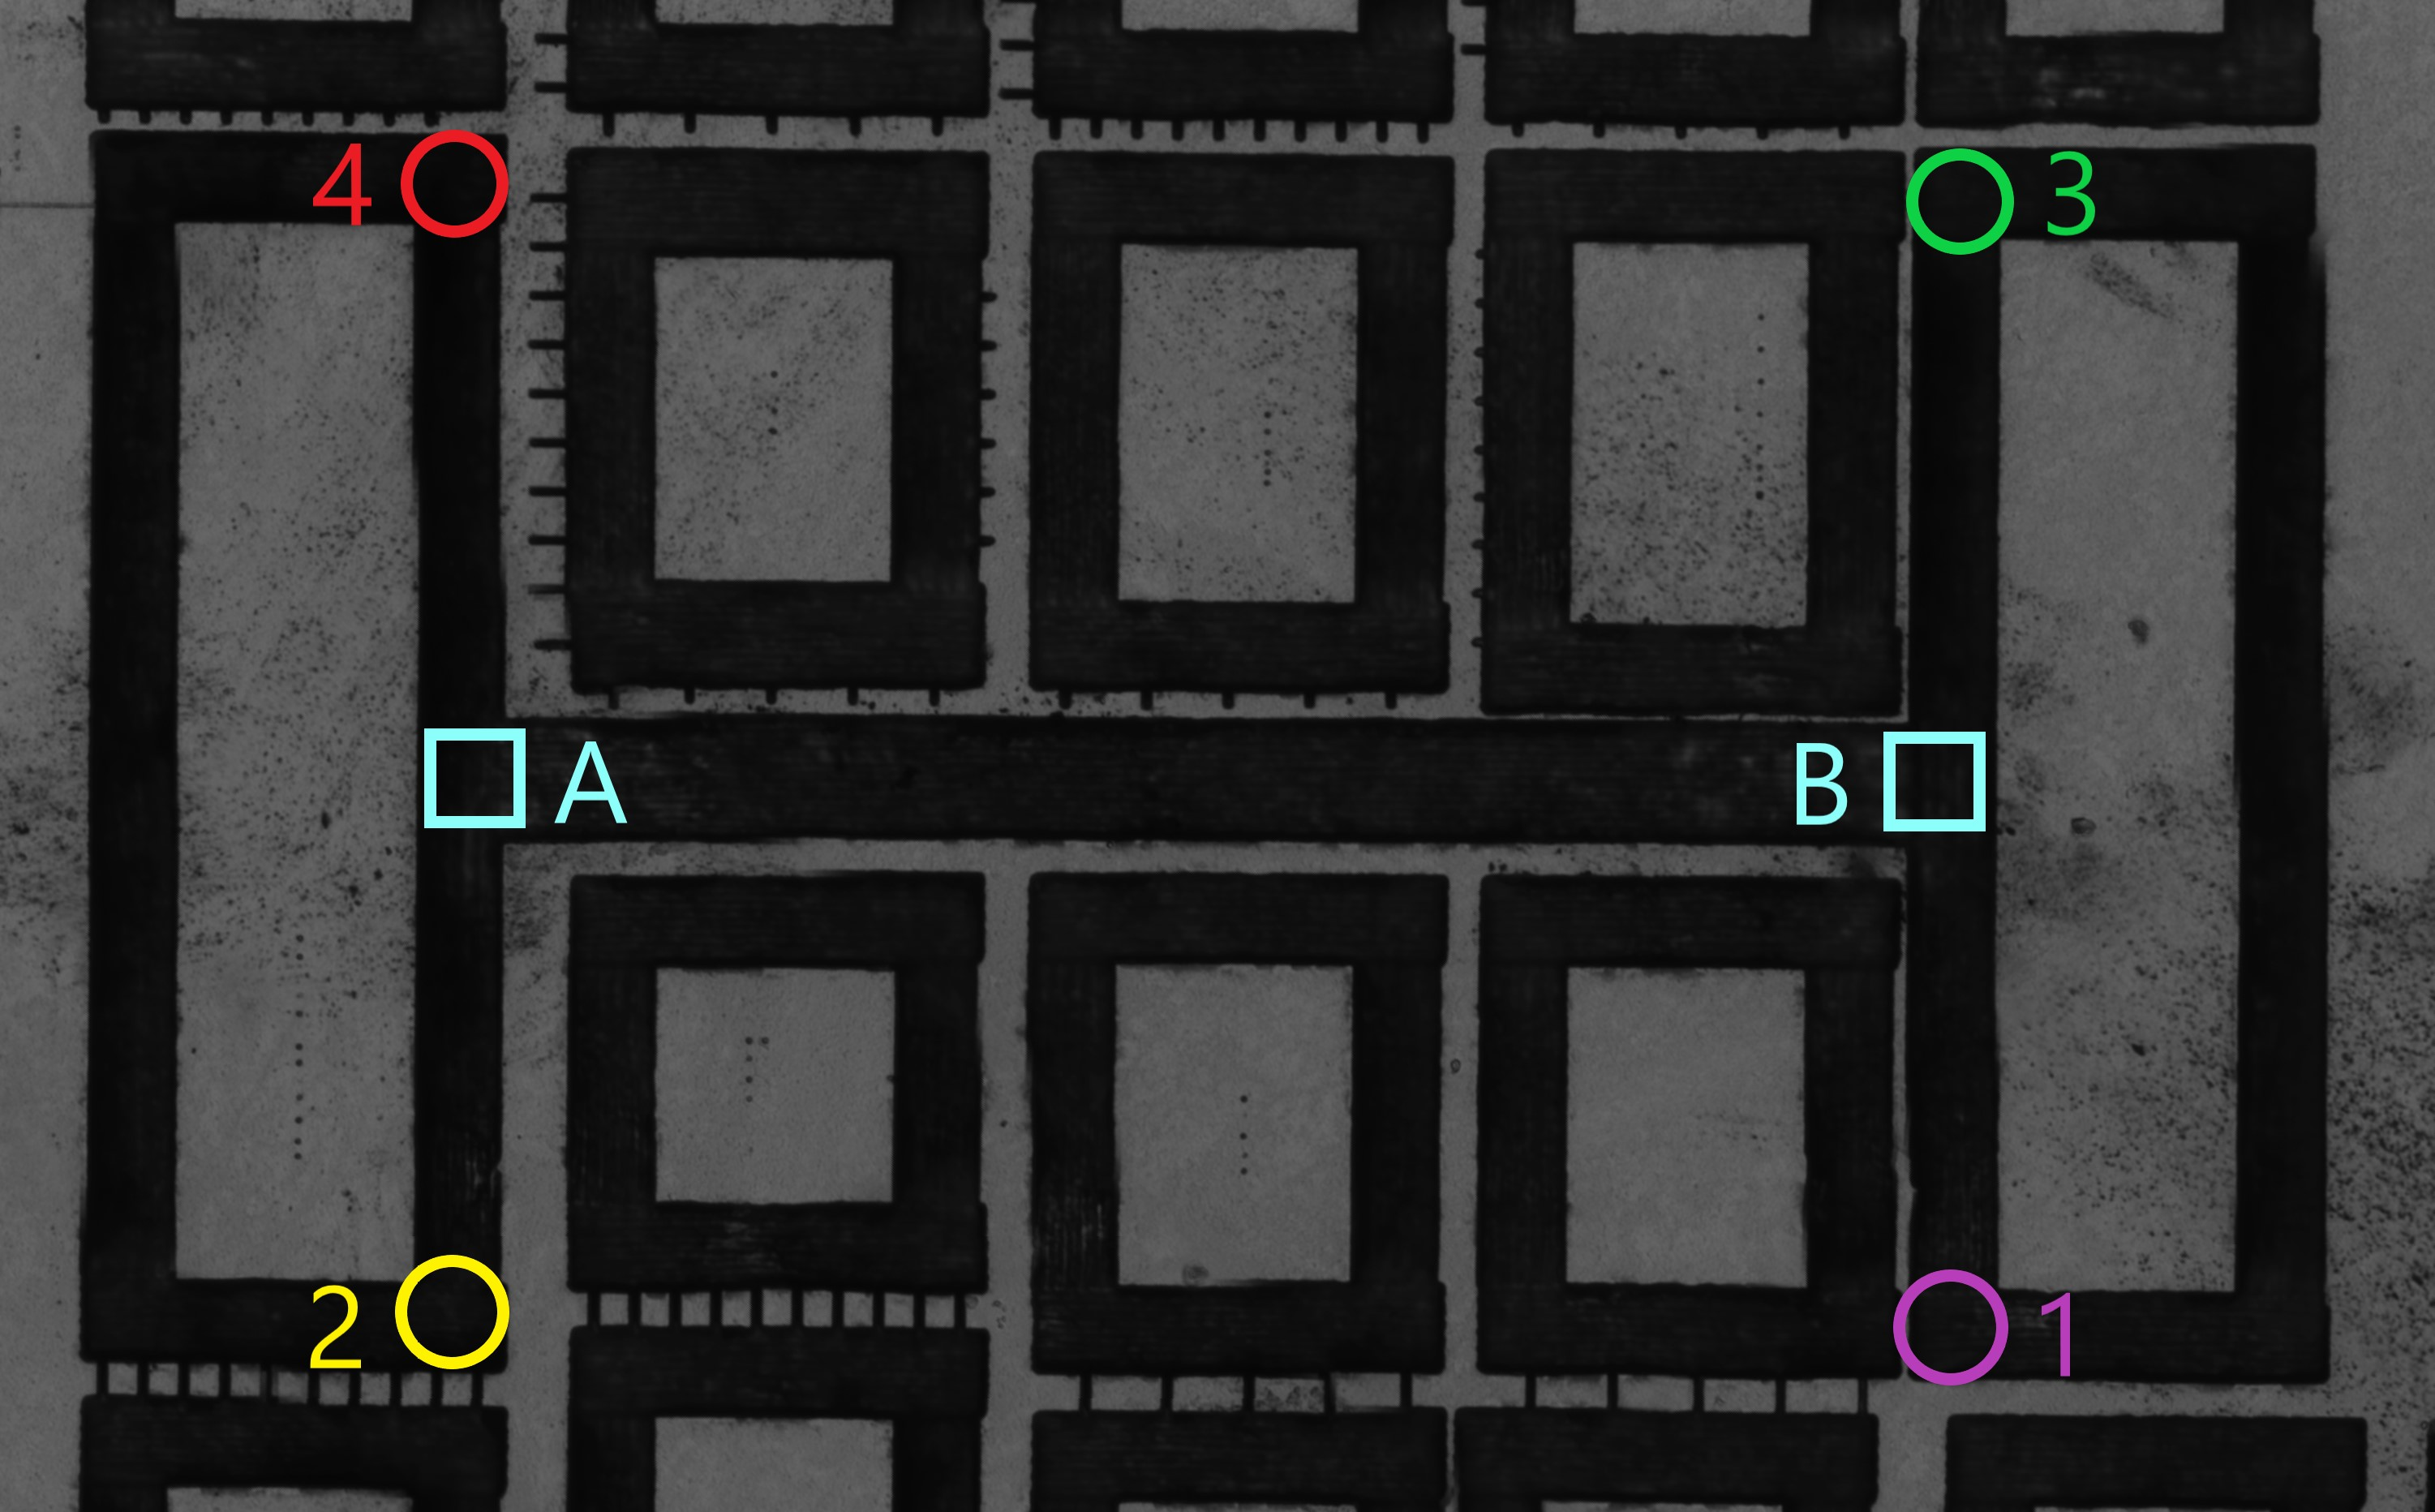
\includegraphics[width=\linewidth]{Chapter7/Figs/Raster/big_bone_esid_annotated.jpg}
    \caption{The I-shaped laser processed conductivity test structure.}
    \label{fig:big_bone_esid}
\end{figure}
Figure \ref{fig:big_bone_esid} shows the simple wire structure that was designed to allow for preliminary electrical characterisation. The annotated shapes indicate the positions of six different electrical probe positions that were used to make contact with the laser processed diamond surface. For reference, these are labelled such that the two aqua squares A and B represent the first set of electrical trials, followed by the circles used for the second set of trials which are labelled 1--4 starting from the bottom right and increasing in the anti-clockwise direction.

As indicated in figure \ref{fig:big_bone_measurements}, the top 10~\si{\micro\metre} wide wires have a length of 70.5~\si{\micro\metre}, and the bottom wire has a length of 65.5~\si{\micro\metre}. This slight difference in path length should result in a reduced resistance in the situation where the induced current is measured across probes 1 and 2, when compared to probes 3 and 4. Note that the 14~\si{\micro\metre} cross-bar wire has a length of 174~\si{\micro\metre} when measured from the edges of the 10~\si{\micro\metre} wires. This substantial length allows for a relatively large distance of laser processed wire to be tested, with the additional benefit of a change in width allowing for comparison with the slightly narrower 10~\si{\micro\metre} wires.
\clearpage
\subsection{Electrical Probe Placement Error Estimation}
\begin{wrapfigure}{r}{0.4\linewidth}
  \centering
  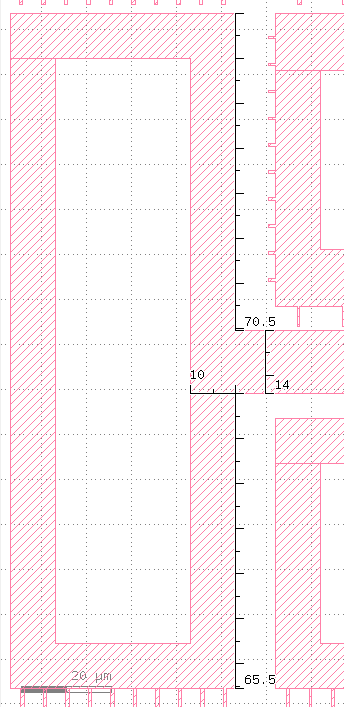
\includegraphics[width=\linewidth]{Chapter7/Figs/Raster/big_bone_measurements_2.png}
  \caption{A snippet of the design for the wire testing region.}
  \label{fig:big_bone_measurements}
\end{wrapfigure}
\label{subsubsec:electrical_probe_placement_error_estimation}
One detail worth including at this stage is a discussion of the electrical probe tips that were used to make contact to the laser processed wires. Standard micro-probes usually have tip radii of the order of 10~\si{\micro\metre}, and naturally, trying to make good contact with wires that are 10~\si{\micro\metre} in width is a challenging prospect, especially due to the ablation of material in the centre of the wire. It would be exceedingly difficult to reliably place tips with a diameter greater than that of the surface features in the correct place. Tip placement relies upon the tip curvature and surface topology, which as previously noted is that of surface trenches, of smaller widths than that of the optically observed laser processed wires. It is physically impossible to place such a large tip into the trench, and contact would only be made on the very edges of the probe tip, reducing the surface area of the contact significantly and potentially inducing a large contact resistance if no good contact is formed. For that reason, probe tips with a full tip diameter of 10~\si{\micro\metre} were used to make contact to the surface wire structures directly. The circles used to represent the probe positions in figure \ref{fig:big_bone_esid} hence show a rough approximation of the size of the tips used in the electrical characterisation, with radii at 5~\si{\micro\metre}. 

Despite great care in the positioning of these micro-tips, it is also important to note that the exact positioning of the probes relative to the wires being measured is an important source of error. The exact length of wires under investigation is a crucial variable for the calculation of measured resistivity and conductivity across differing wires. Hence, the variation of micron-scale positioning must be accounted for. The minimum potential error in electrical path length may be given by $2\times$ the tip radii, which is $\pm10$~\si{\micro\metre}. This is the minimum due to the tip radii themselves, but also sets a lower bound for the potential of inexact placements during the experimental process itself, as the probe tips may not necessarily be ideally situated in the locations marked on figure \ref{fig:big_bone_esid}. While the placements were aided by an optical microscope, the precision and reliability with micropositioners establishes a hard limit of $\pm5$~\si{\micro\metre} per probe tip. In particular for these smaller than average probe tip radii, the identification of physical contact was challenging to observe, with any additional force applied to the probe leading to significant bending of the probe tip and subsequent translation of the probe tip along the wire. Larger tip radii allows for a probe tip with greater resistance to deformation, but as previously discussed the tip radii was strategically chosen to allow for the best possible contacts to be made to 10~\si{\micro\metre} wide wires, leading to this potential error in placement but reducing the issue of contact formation itself.

\begin{table}[ht]
\centering
\begin{tabular}{|c|c|c|c|}
\hline
Electrical Path & Path Length (\si{\micro\metre}) \\
\hline
A-B & $164$  \\
1-3 & $140$  \\
2-4 & $140$  \\
1-2 & $295$  \\
3-4 & $305$  \\
1-4 & $301$  \\
3-2 & $301$  \\
\hline
\end{tabular}
\caption{Summary of electrical path lengths and the corresponding error due to probe placement. The error in path length is taken as $\pm10$.}
\label{table:probe_placement_error}
\end{table}

Table \ref{table:probe_placement_error} provides a brief summary of the electrical path lengths between the different probe locations. The standard minimum error is more notable for the shortest electrical paths, such as A-B or 1-3, 2-4, when it is expressed as a percentage error of the path length. However, by taking this into account the conclusions of electrical measurements taken between these probe locations can be considered fairly.

\subsection{Laser Writing Thickness}
\label{subsubsec:laser_writing_thickness}
One final detail is necessary to consider the effective resistivity of the laser processed surface wires -- that of the thickness of these processed regions. A full overview of the laser processing technique is outlined more fully in section \ref{sec:laser}, however the salient point regarding laser treated thickness can be estimated based on key studies in which the structure of laser processed diamond samples are examined via techniques such as TEM \cite{salter2017}, SEM \cite{ashikkalieva2022} and interference based microscopy techniques following the removal via oxidation of graphitic material \cite{kononenko2005}. Despite the topological complications induced by ablation during the laser processing technique, it is reasonable to estimate based on this prior work that the thickness of material in which a graphitisation or general sp$^{3}$ bond breaking process has occurred is likely to be relatively continuous, with only small variations on average across the laser treated region. With consideration of the literature that is comparable to the laser processing performed to create these device structures \cite{kononenko2005, Kononenko2009, kononenko:2015}, a simple assumption that will allow for further analysis of the electrical properties of laser written wires is to take an estimated thickness of 500~\si{\nano\metre} for the effective thickness. This then represents material that may be considered to contain graphitised phases of carbon. This is consistent with the photographitisation/thermal graphitisation process that is described in section \ref{sec:laser}, though it must be stated that the exact thickness of the graphitised material will be a function of position along the wire, and it is unlikely to be completely uniform. 

\begin{figure}[H]
    \centering
    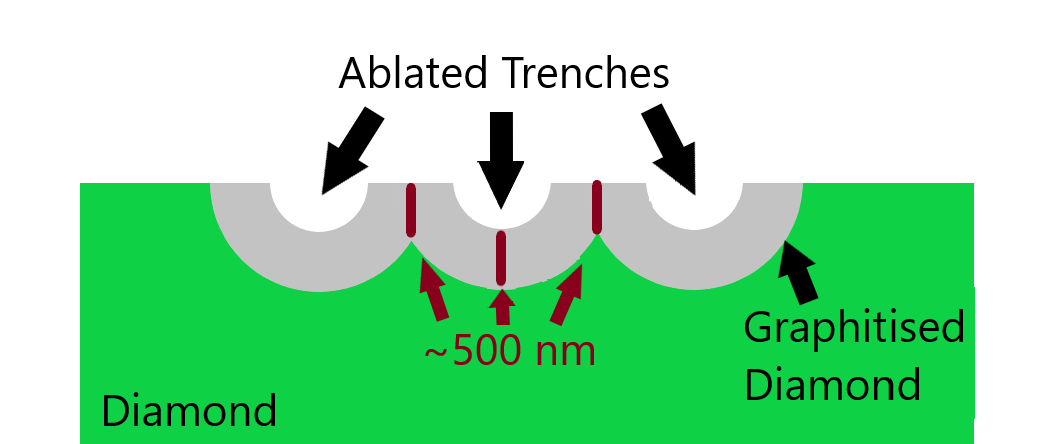
\includegraphics[width=\linewidth]{Chapter7/Figs/Raster/simple_ablation_model_2.png}
    \caption{A simple ablation model to demonstrate the approximate thickness of graphitic material.}
    \label{fig:simple_ablation_model_2}
\end{figure}

A rudimentary model of the thickness approximation is represented in figure \ref{fig:simple_ablation_model_2}. There are a few complications that must be acknowledged with such a model. First, the order in which the laser processing is performed will affect the photographitisation/thermal graphitisation process itself, with additional ablation occurring when laser treatment is applied adjacent to a point which already has a significant degree of graphitisation. This may be one of the most significant reasons as to why the profile of laser treated surface wires shows one deep topological trench, with a roughness that may then be due to the individual ablation regions. 

Second, the spacing between adjacent laser spots will naturally change the ablation regions, and surface topology, with knock on effects for the graphitised region of interest. If laser spots are kept very close together, then the semi-circles representing ablated trenches in figure \ref{fig:simple_ablation_model_2} will overlap, with a non-trivial local thickness of the graphitised region in these regions of overlap. 

Thirdly, the photographitisation process is quite dependent upon defects as the origin of sp$^{3}$ bond breaking \cite{kononenko2014-PI}, in material which contains said defects. There are multiple defects that could have formed the origin of such photo-induced graphitisation, such as at the interface between the HPHT substrate and CVD grown heavily phosphorous doped diamond film \cite{tallaire2011}, within the CVD grown layer itself due to the growth conditions used for highly phosphorus doped material \cite{grotjohn2014}, and the HPHT substrate itself due to the nitrogen content and likely high density of twinning or stacking faults \cite{Angus1992, sumiya2015}. Hence, the origin of photographitisation is difficult to ascertain in such a substrate, and this may lead to a small amount of variance in the depth at which the sp$^{2}$ seeds are formed. The relative consistency of the topological scans demonstrated thus far indicates that despite these complications in a more precise model of the thickness of graphitised material, the ablation within the wider wires where multiple passes of laser processing has occurred is reasonably consistent. This removes the third point from relevance, as the exact positioning of the photo-induced graphitisation process need not be considered a large factor. 

While the first and second points still hold, comparison to previous work indicates that while there may be some variability in the local thickness of laser graphitised layers, the approximate thickness of 500~\si{\nano\metre} should provide a reasonable estimate of the resistivity of these layers. At minimum, there should not be any points within the laser written wires where there is a thickness substantially thinner than 500~\si{\nano\metre}, with large deviations likely to be slightly thicker than this estimate. 

\subsection{Conductive Wire Testing - 14 micron width}
\label{subsubsec:graphitised_wire_testing_14}
\begin{figure}[H]
    \centering
    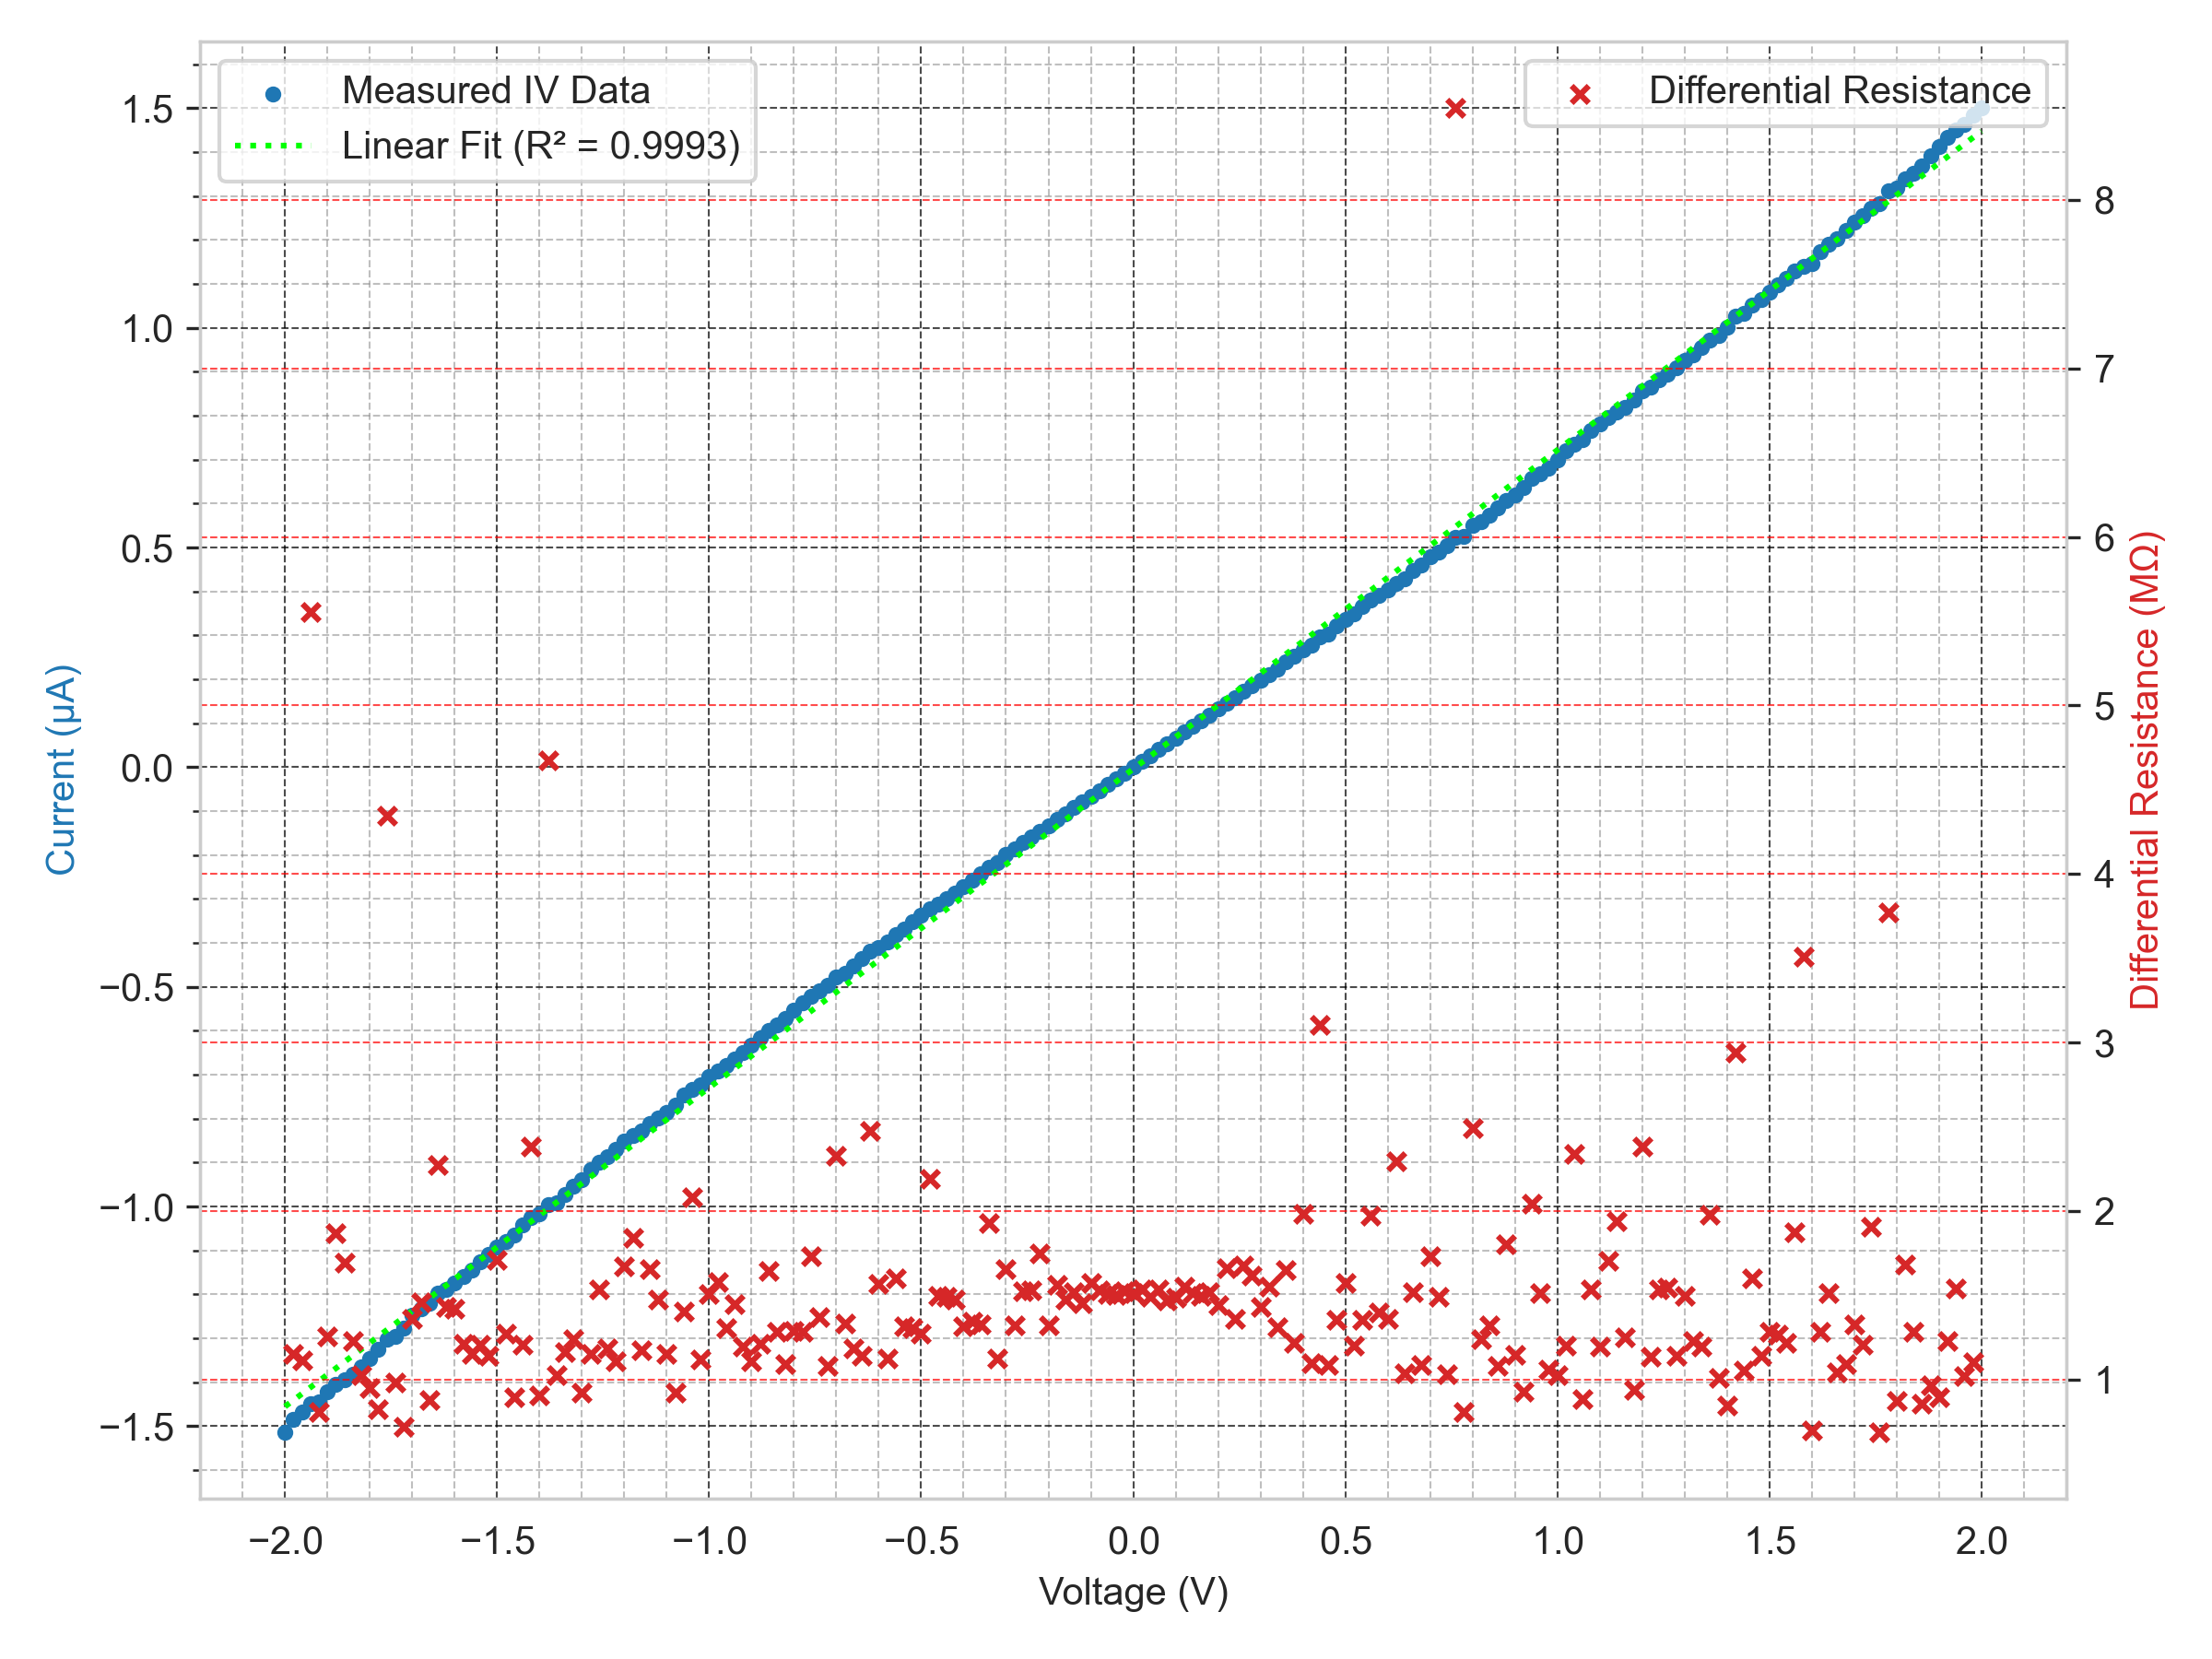
\includegraphics[width=\linewidth]{Chapter7/Figs/Raster/2V AB d.png}
    \caption{The first set of electrical measurements across the 14~\si{\micro\metre} wire structure via probe locations A and B.}
    \label{fig:2v_ab}
\end{figure}
The first set of electrical measurements were carried out between probe positions A and B as shown in figure \ref{fig:big_bone_esid}. The linear IV plot is shown in figure \ref{fig:2v_ab}, and shows a good ohmic relationship in the low voltage region of $\pm$ 2~\si{\volt} (R$^{2} = 0.9993$). This line of best fit corresponds to a measured total resistance of $1.34$~\si{\mega\ohm}. A full set of electrical measurements were taken from this starting point, increasing up to an absolute potential bias of 100~\si{\volt} applied at probe A, with probe B held at ground. Figure \ref{fig:2v_ab} also displays the differential resistance between consecutive data points, further demonstrating the ohmic quality of this wire.

\begin{figure}[H]
    \centering
    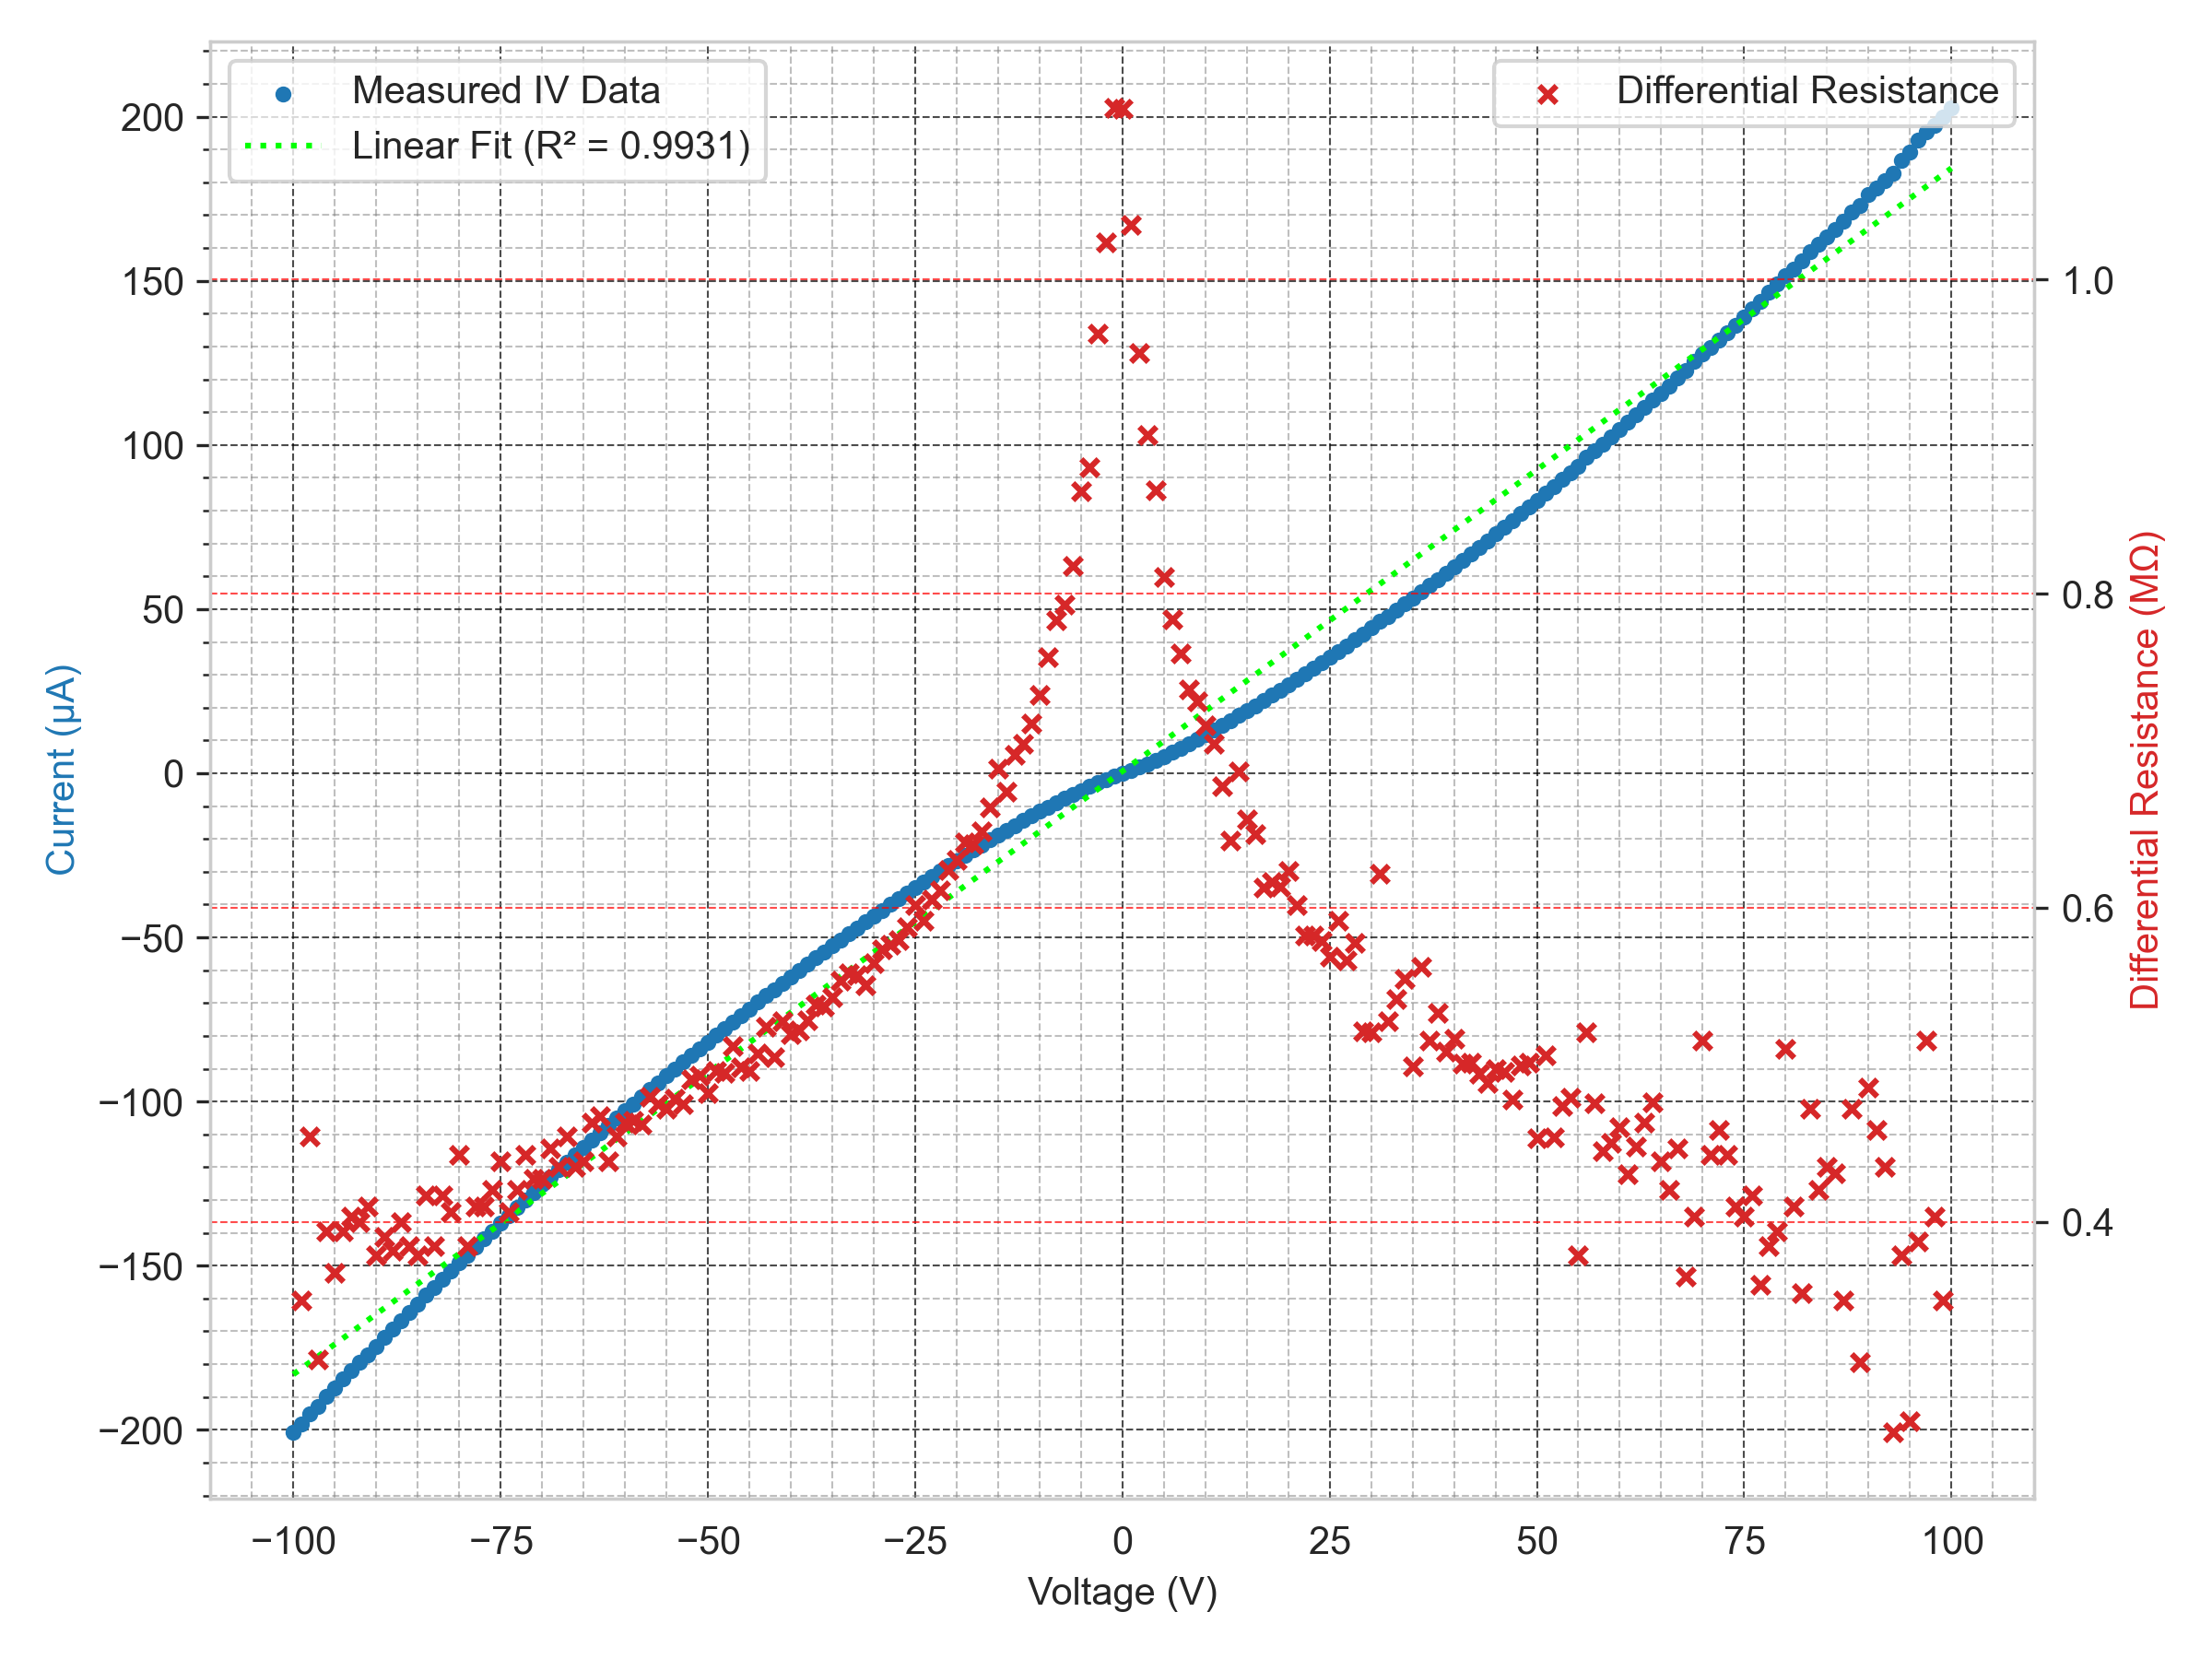
\includegraphics[width=\linewidth]{Chapter7/Figs/Raster/100V AB d.png}
    \caption{A $\pm$100~\si{\volt} set of electrical measurements across the 14~\si{\micro\metre} wire structure via probe locations A and B.}
    \label{fig:100v_ab}
\end{figure}

\begin{table}[ht]
\centering
\begin{tabular}{|c|c|c|c|c|}
\hline
Voltage (V) & Total Resistance (M$\Omega$) & Diff. in Resistance (k$\Omega$) & Absolute \% Diff. & R² \\
\hline
2  & $1.38$ & $14.9$ & 1.08\% & 0.9993 \\
5  & $1.21$ & $-19.8$ & 1.64\% & 0.9964 \\
10 & $0.992$ & $-16.1$ & 1.62\% & 0.9925 \\
20 & $0.771$ & $11.6$ & 1.50\% & 0.9930 \\
40 & $0.629$ & $6.18$ & 0.98\% & 0.9914 \\
60 & $0.589$ & $16.8$ & 2.85\% & 0.9933 \\
80 & $0.571$ & $-14.0$ & 2.45\% & 0.9937 \\
100& $0.544$ & $-5.57$ & 1.02\% & 0.9931 \\
\hline
\end{tabular}
\caption{Total resistance, difference in positive vs negative resistances, the absolute percentage difference, and total R$^{2}$ for various voltage ranges.}
\label{tab:resistance_difference_total}
\end{table}

Figure \ref{fig:100v_ab} shows the electrical characteristics when measured with a potential bias of $\pm100$~\si{\volt}. In contrast to the lower voltage range, a Schottky behaviour can be observed. The linear fit yields an R$^{2}$ value of 0.9931, and a measured total resistance for this linear fit of $0.544$~\si{\mega\ohm}. One valuable thing to consider with these characteristics is the potential for asymmetry in the measured resistance, and how this may change as the voltage range changes. To examine this briefly, table \ref{tab:resistance_difference_total} collects the calculated difference in resistance between the positive and negative regions, which may be expressed as $R_{\text{diff}} = R_{+} - R_{-}$, and also shows the percentage difference between the absolute value of $R_{\text{diff}}$ and the resistance as calculated from the full fit for the dataset $\left(\frac{\left| R_{\text{diff}} \right|}{R_{\text{total}}} \times 100\%\right)$. The results indicate that the data are well regarded as symmetric in nature, with only minor absolute \% differences between the resistance as measured from the positive and negative voltage regions. There doesn't appear to be any clear correlation between the change in sign for $R_{\text(diff)}$ and the voltage range used, though it is also difficult to state that this is due to noise or other such error in the measurements, since the absolute \% difference changes across the voltage range used. 

The examination of symmetry will be explored further with the electrical characterisation of emitter structures, due to the possibility of one-way diodes being created through the geometric field enhancement and subsequent field effect emission. However, in this case, both probes A and B are placed on what is ostensibly material containing enough graphitic phase carbon to allow for near-ohmic conductivity. The observation of an inconsistent asymmetry may indicate some change in the structure of sp$^{2}$ phase carbon under the application of electrical bias, or potentially a more exotic phase of carbon such as a diaphitic structure. This will be explored further later in this chapter.

\begin{figure}[H]
    \centering
    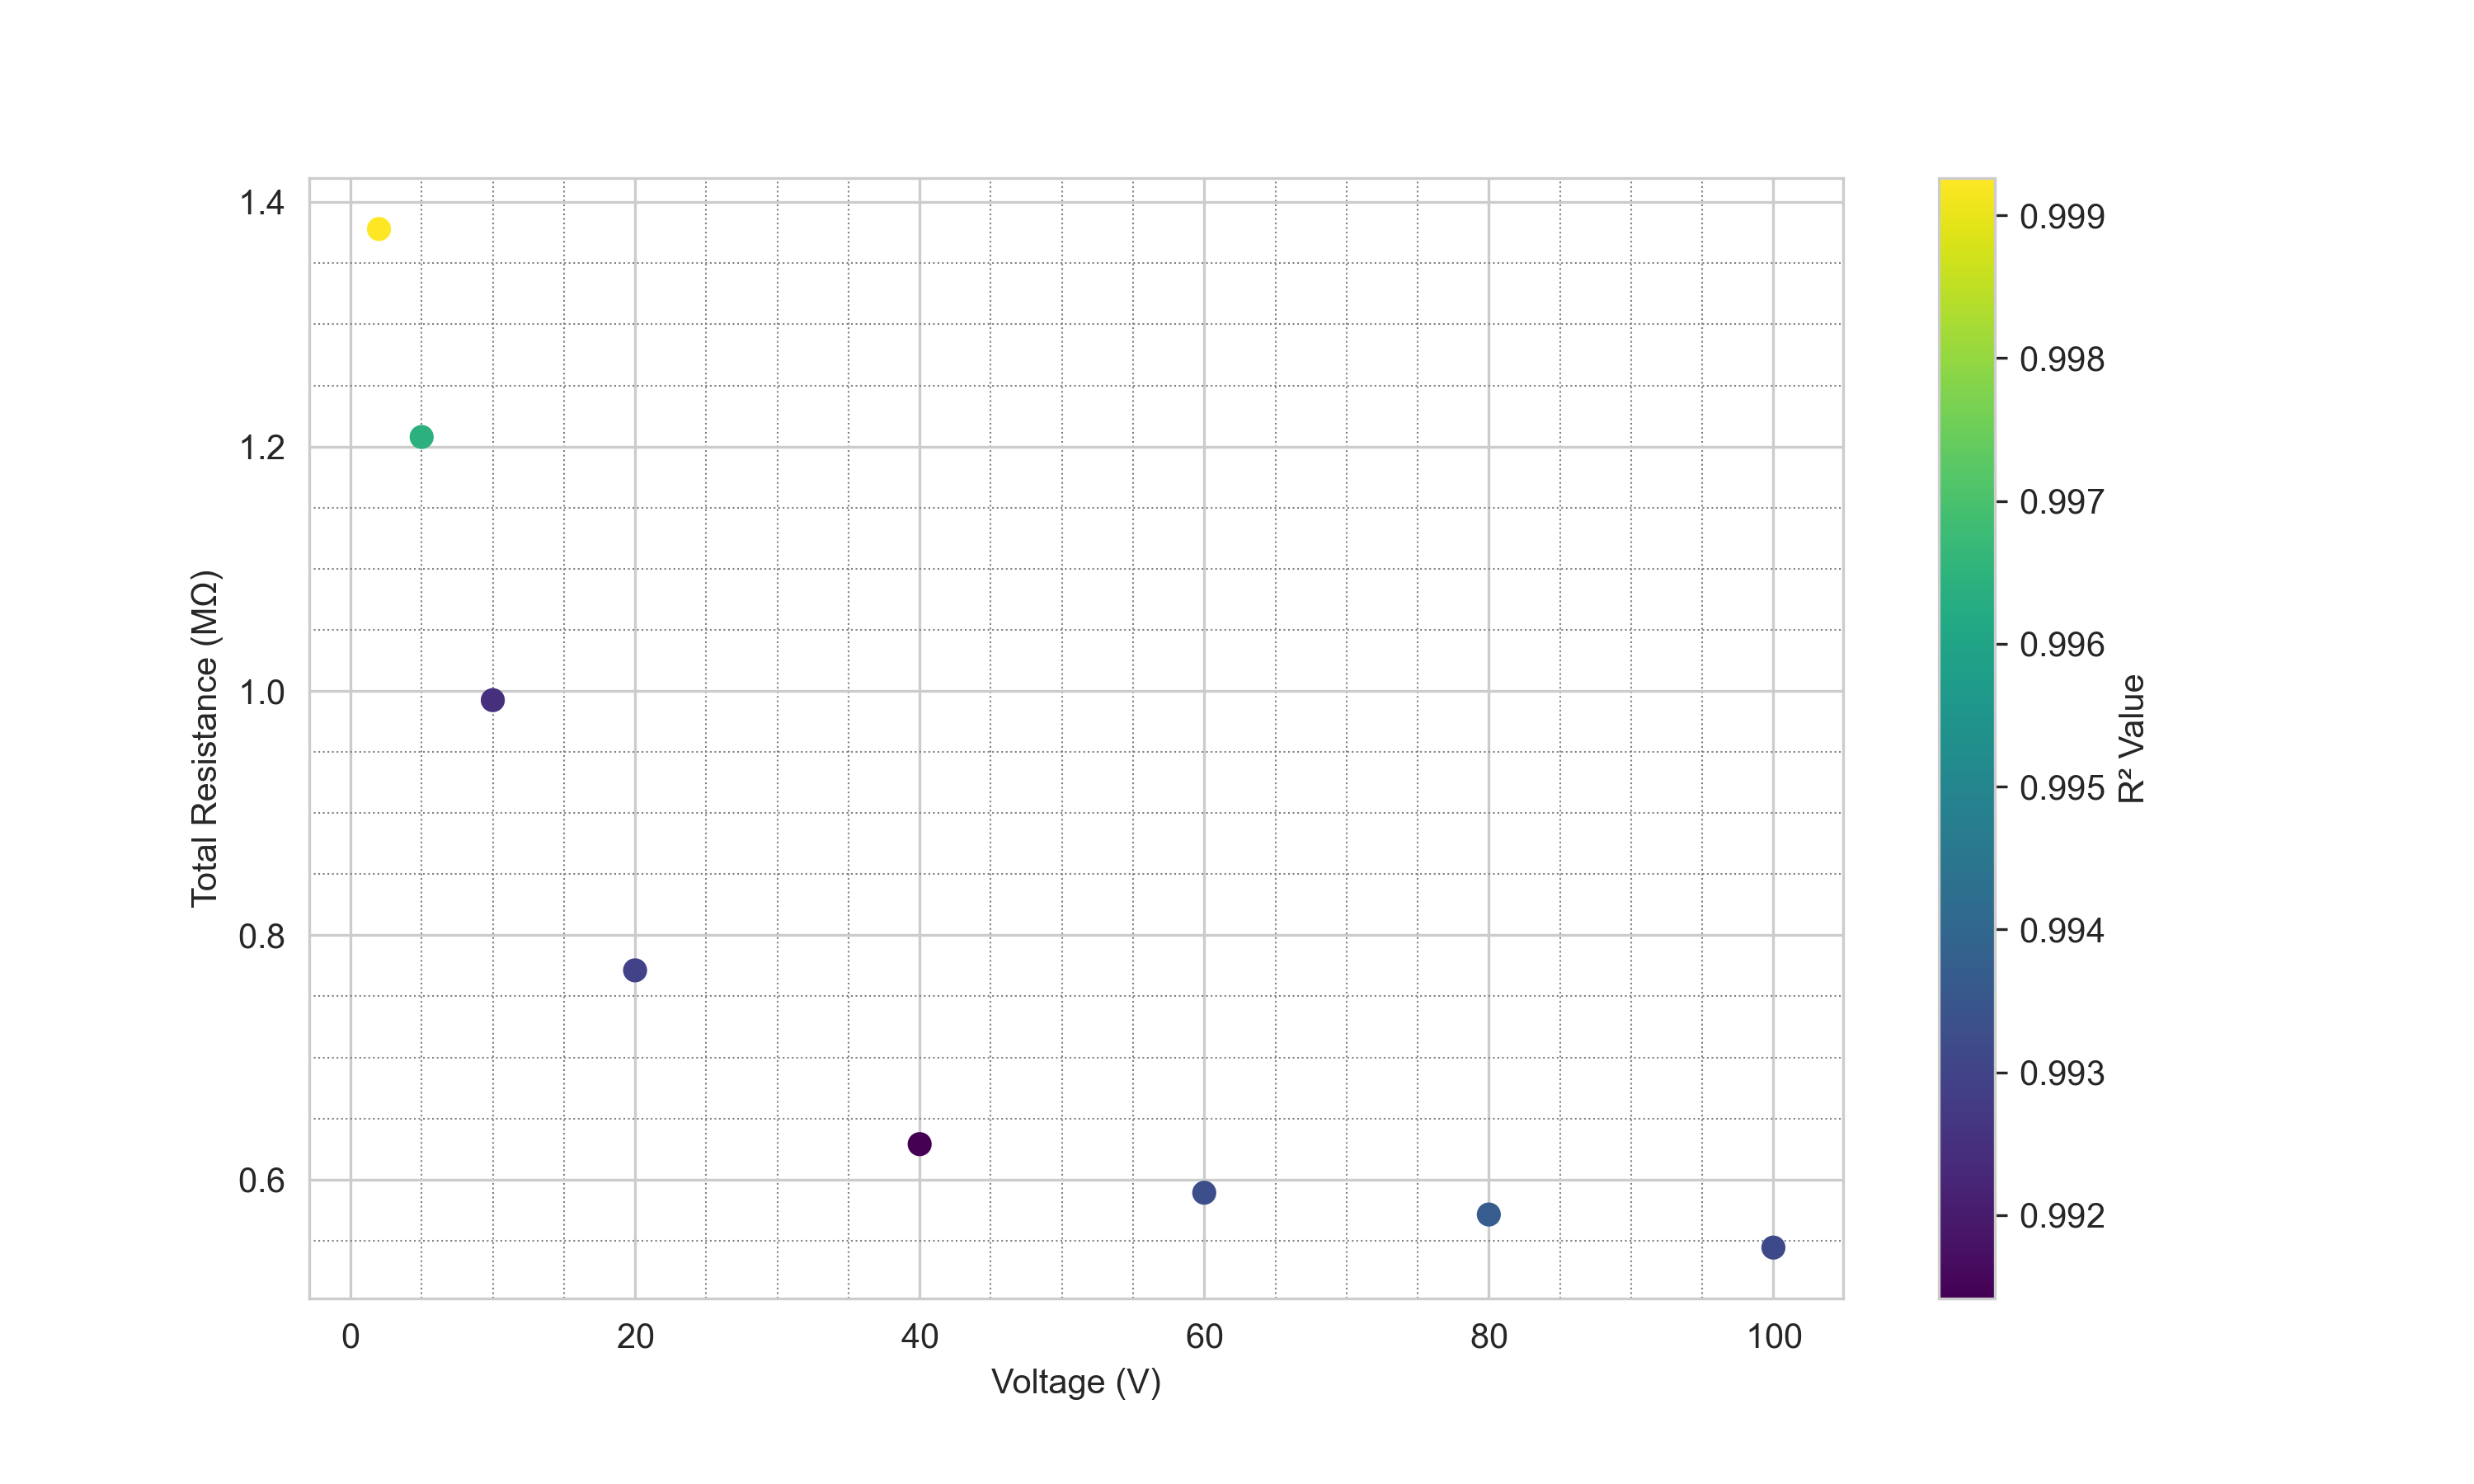
\includegraphics[width=\linewidth]{Chapter7/Figs/Raster/full_range AB.png}
    \caption{The full voltage range and their corresponding total resistances as measured across probes A and B.}
    \label{fig:full_range_ab}
\end{figure}

Figure \ref{fig:full_range_ab} displays the full range of measured total resistances based on the voltage range used. A colour scale is used to represent the changing R$^{2}$ value as the IV characteristics trend towards a Schottky-like behaviour at higher voltage ranges, deviating from the linear fit applied for the calculation of resistance.

\begin{table}[ht]
\centering
\begin{tabular}{|c|c|c|c|}
\hline
Voltage (V) & Resistivity ($\Omega$cm) & Conductivity (S/m) & Conductivity Error (S/m) \\
\hline
2 & $5.88$ & $17.0$ & $1.04$ \\
5 & $5.16$ & $19.4$ & $1.18$ \\
10 & $4.24$ & $23.6$ & $1.44$ \\
20 & $3.29$ & $30.4$ & $1.85$ \\
40 & $2.68$ & $37.2$ & $2.27$ \\
60 & $2.51$ & $39.8$ & $2.43$ \\
80 & $2.44$ & $41.0$ & $2.50$ \\
100& $2.32$ & $43.0$ & $2.62$ \\
\hline
\end{tabular}
\caption{Voltage vs. resistivity, conductivity, and a conductivity error of 6.1\% for this wire.}
\label{table:ab_resistivity_conductivity}
\end{table}

Table \ref{table:ab_resistivity_conductivity} shows the resulting resistivity and conductivity as measured across the various voltage ranges between probes A and B. Immediate comparisons could be made to typical conductivity values for graphite, which, when parallel to the basal plane are typically reported to have values of 2--4$\times10^{5}$~\si{\siemens\per\metre}, and perpendicular to the basal plane are closer to $333$~\si{\siemens\per\metre} \cite{pierson1993}. The best reported conductivity here at a bias of 100~\si{\volt} is of $43.0$~\si{\siemens\per\metre}, approximately 8 times smaller than that of the perpendicular graphite conductivity value. This is a significantly higher conductivity than that of the diamond substrate itself as measured via LTLM and CTLM in chapter \ref{ch:electrical_experiments} on another sample with a heavily phosphorous doped surface layer grown under the same conditions as for this sample. However, it is difficult to infer the dominant form of carbon allotrope that is present, especially when the concept of electrical percolation within composite materials is considered as in \cite{mclachlan1990}. The recent application of complex network theory to electrical conduction mechanisms in nanostructure assemblies allows for a wide range of conduction types, even in materials that at first appear to be discontinuous \cite{yao2020}. Hence, the reduced resistivity observed in laser treated diamond that contains a larger content of sp$^{2}$ bonded carbon would appear to show that, despite not being a truly "graphitic" wire that acts as a metal, with conductivity similar to that of bulk graphite, enough electrically conductive material is present to allow for ohmic conductivity, albeit with a higher resistance than might be expected.

\begin{figure}[H]
    \centering
    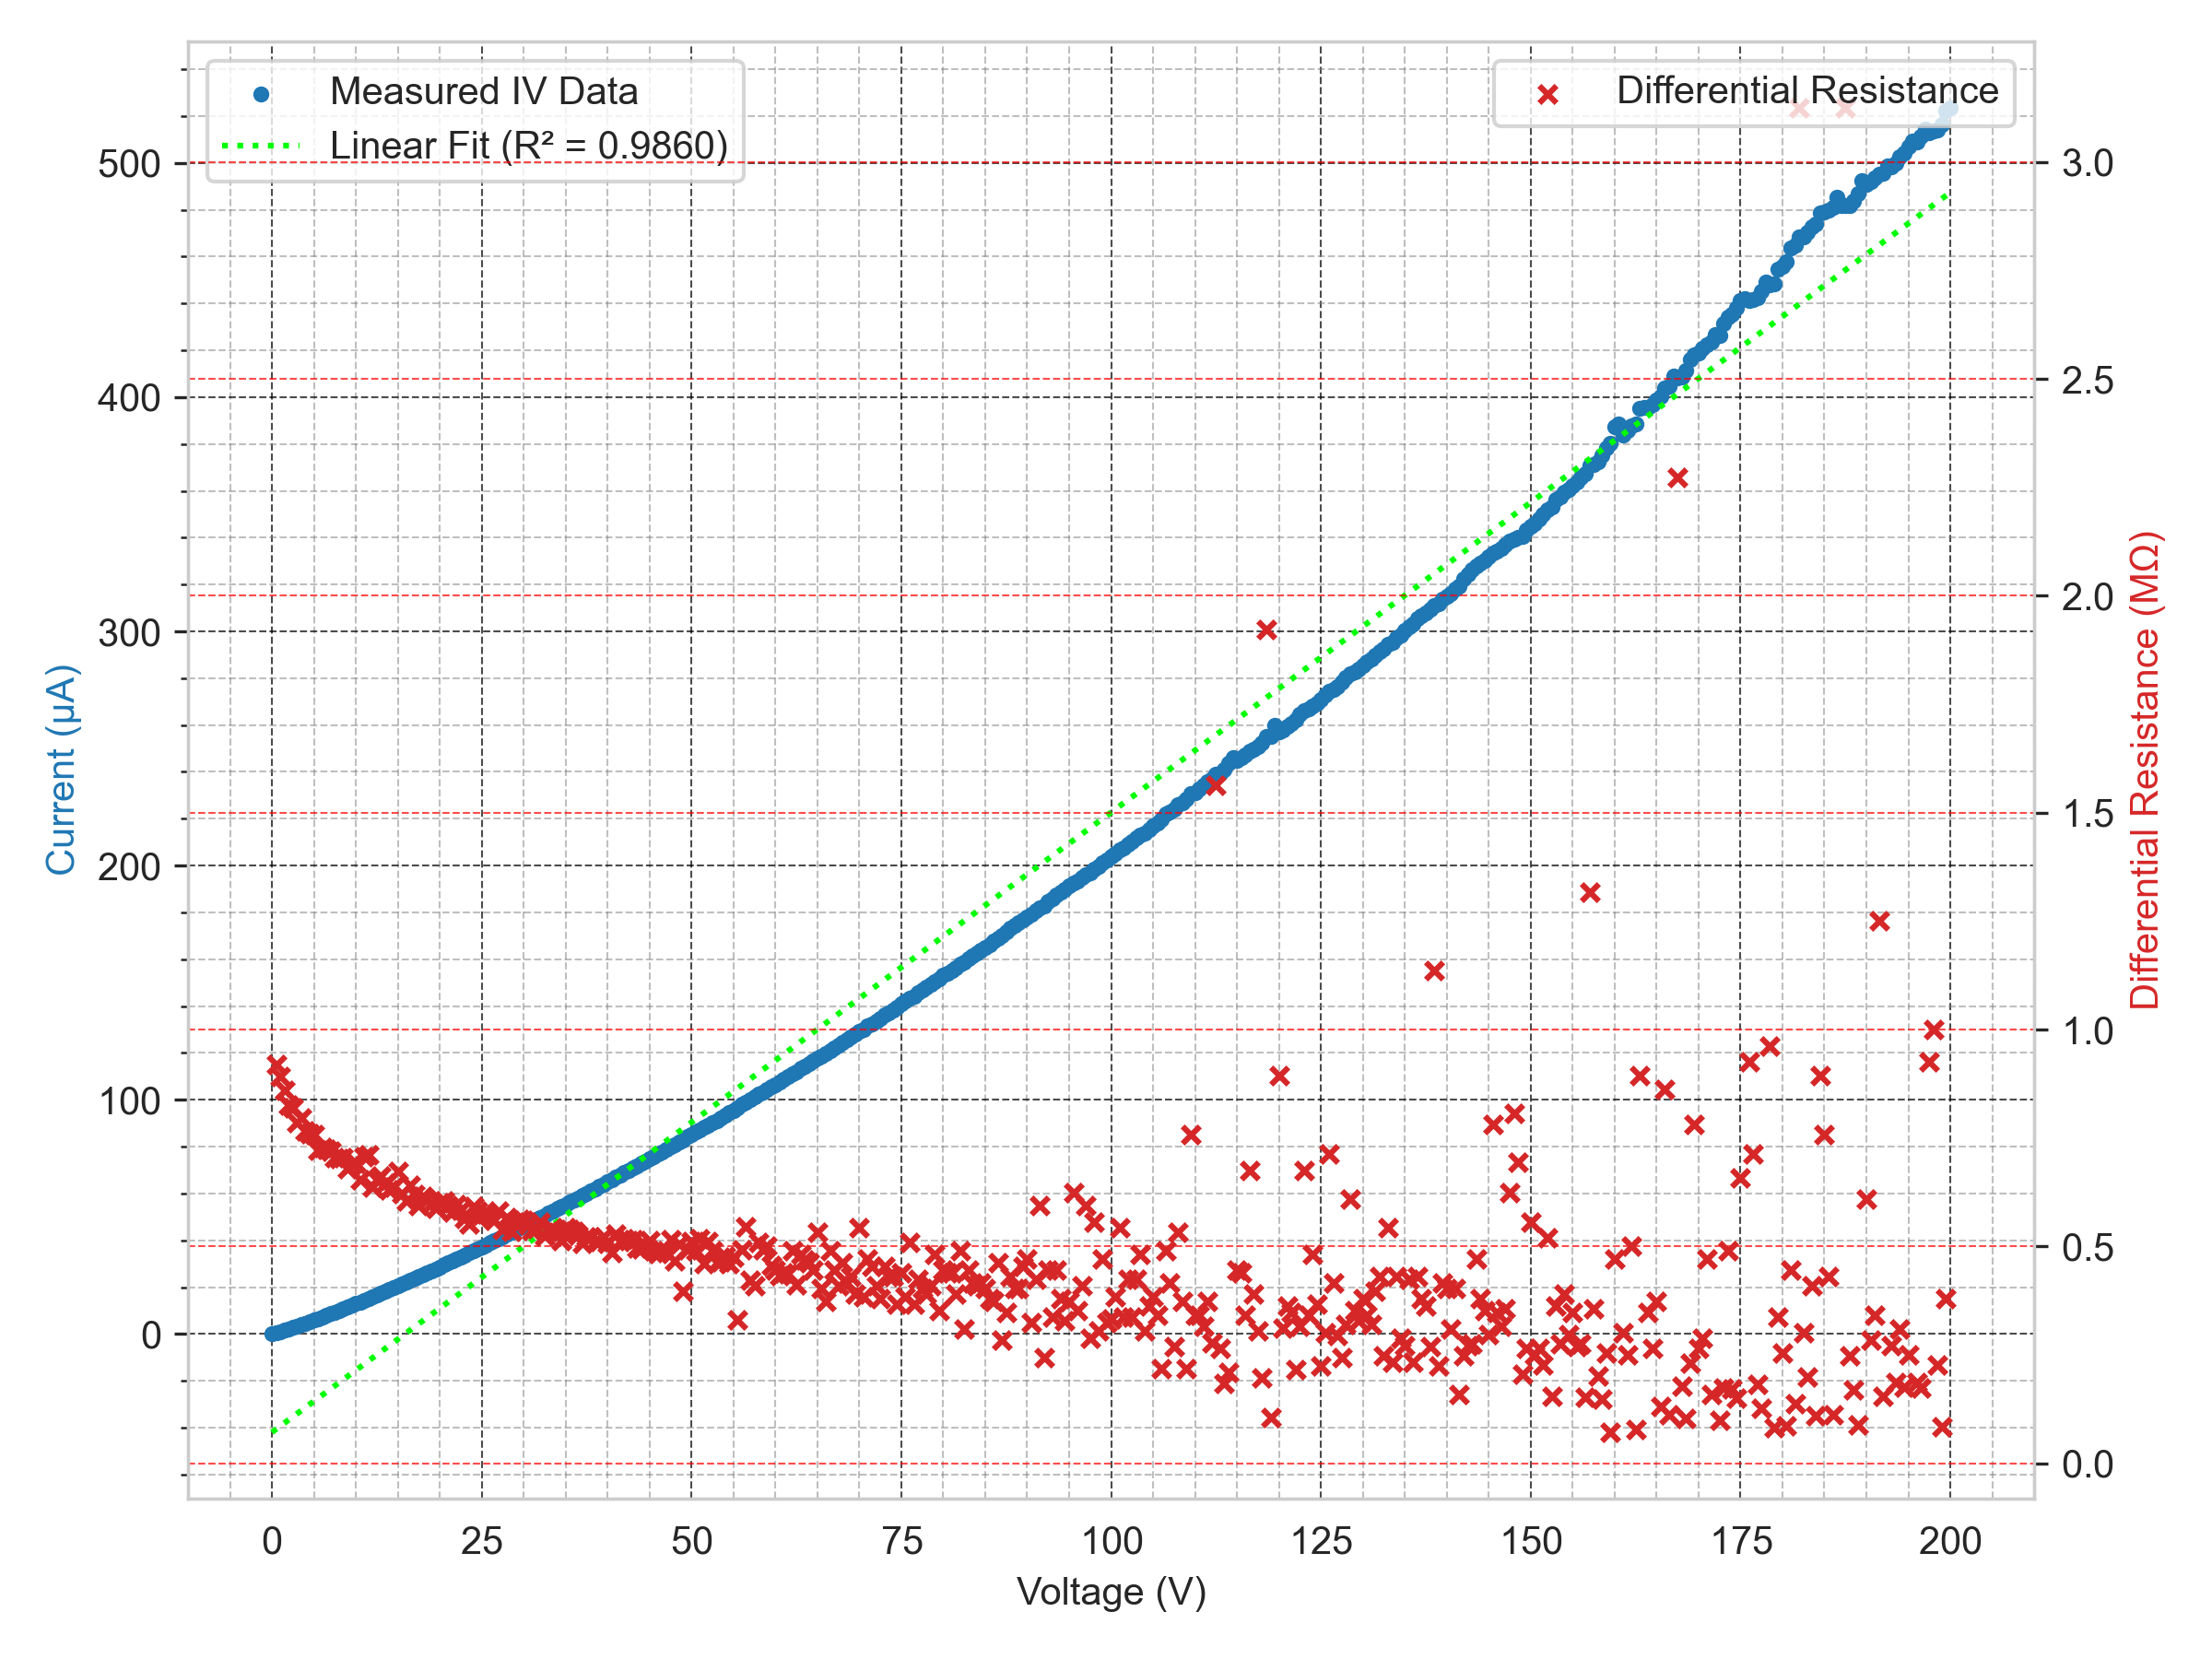
\includegraphics[width=\linewidth]{Chapter7/Figs/Raster/200V AB d.png}
    \caption{A set of electrical measurements across the 14~\si{\micro\metre} wire structure via probe locations A and B, reaching up to 200~\si{\volt}.}
    \label{fig:200v_ab}
\end{figure}

\begin{table}[ht]
\centering
\begin{tabular}{|c|c|c|c|}
\hline
Voltage (V) & Resistivity ($\Omega$cm) & Conductivity (S/m) & Conductivity Error (S/m) \\
\hline
4 & 4.06 & 24.6 & 1.50 \\
10 & 3.51 & 28.5 & 1.74 \\
20 & 3.07 & 32.6 & 1.99 \\
40 & 2.64 & 37.9 & 2.31 \\
60 & 2.38 & 42.0 & 2.56 \\
80 & 2.20 & 45.4 & 2.77 \\
100 & 2.09 & 47.8 & 2.92 \\
120 & 1.99 & 50.3 & 3.07 \\
140 & 1.89 & 52.8 & 3.22 \\
160 & 1.80 & 55.5 & 3.39 \\
180 & 1.73 & 57.9 & 3.53 \\
200 & 1.61 & 62.0 & 3.78 \\
\hline
\end{tabular}
\caption{Total voltage sweep vs. resistivity, conductivity, and a conductivity error of 6.1\% for the wire.}
\label{table:total_sweep_resistivity_conductivity}
\end{table}

Next, higher voltage testing was performed, which continued the same observations as outlined in table \ref{table:ab_resistivity_conductivity}. An example of a 200~\si{\volt} sweep is shown in figure \ref{fig:200v_ab}, with a linear fit corresponding to a measured resistance of $3.78\times10^{5}$~\si{\ohm} plotted alongside the raw data. The Schottky-like behaviour continues to grow in significance at these higher voltages, with more deviation from the linear fit visible. However, the effective conductivity continues in much the same trend as before, with a conductivity of 62~\si{\siemens\per\metre} from the linear fit. This is represented in figure \ref{fig:200v_ab} by the decrease in differential resistance at higher voltages.

Table \ref{table:total_sweep_resistivity_conductivity} gives the full set of higher voltage data between probes A and B. This set of measurements was performed with fresh probe tips and a complete reset of the experimental setup, to ensure that the results were not dependent upon an unknown error related to the previous set of result. Similar to the previous measurements, the conductivity at a bias of 10~\si{\volt} was around $28.5\pm1.7$~\si{\siemens\per\metre}. One notable difference with these measurements is the setting of the ground probe to a negative bias, rather than holding it at ground. This allowed for a wider range of potential biases to be explored with the electrical probe station, but prevented the previous estimation of asymmetrical differences in absolute current values for negative vs positive electrical biases.

\subsection{Conductive Wire Testing - 10 microns}
\label{subsubsec:graphitised_wire_testing_10}
In the previous section, the calculation of effective conductivity for the large (14~\si{\micro\metre}) laser processed wire is set out as for the measurements taken between probe locations A and B. Further measurements were taken at probe locations 1--4, following the electrical measurements of A--B. One small detail, which was noticed during the testing of A--B was that following multiple voltage sweeps at higher potential differences, the observed conductivity appeared to decrease marginally across multiple sweeps. However, testing the following day was able to achieve similar results to that set out in table \ref{table:ab_resistivity_conductivity}. Regardless, it is worth examining the measurements between probe locations 1-4 and 2-3 separately, as these wires were otherwise untested in the previous conductivity measurements between probes A and B. They also have a different wire thickness of 10~\si{\micro\metre}, and so it may be natural to expect a higher resistivity. The comparative values of the wires are $3.57\times10^{-8}$~\si{\metre} for the 10~\si{\micro\metre} wires and $4.27\times10^{-8}$~\si{\metre} for the 14~\si{\micro\metre} wire. Hence, if the wires do indeed follow the trivial calculation of resistivity using an estimated thickness of 500~\si{\nano\metre}, it is expected that these thinner wires will show a conductivity that is approximately 16\% lower than that of the 14~\si{\micro\metre} wires.

\begin{figure}[H]
    \centering
    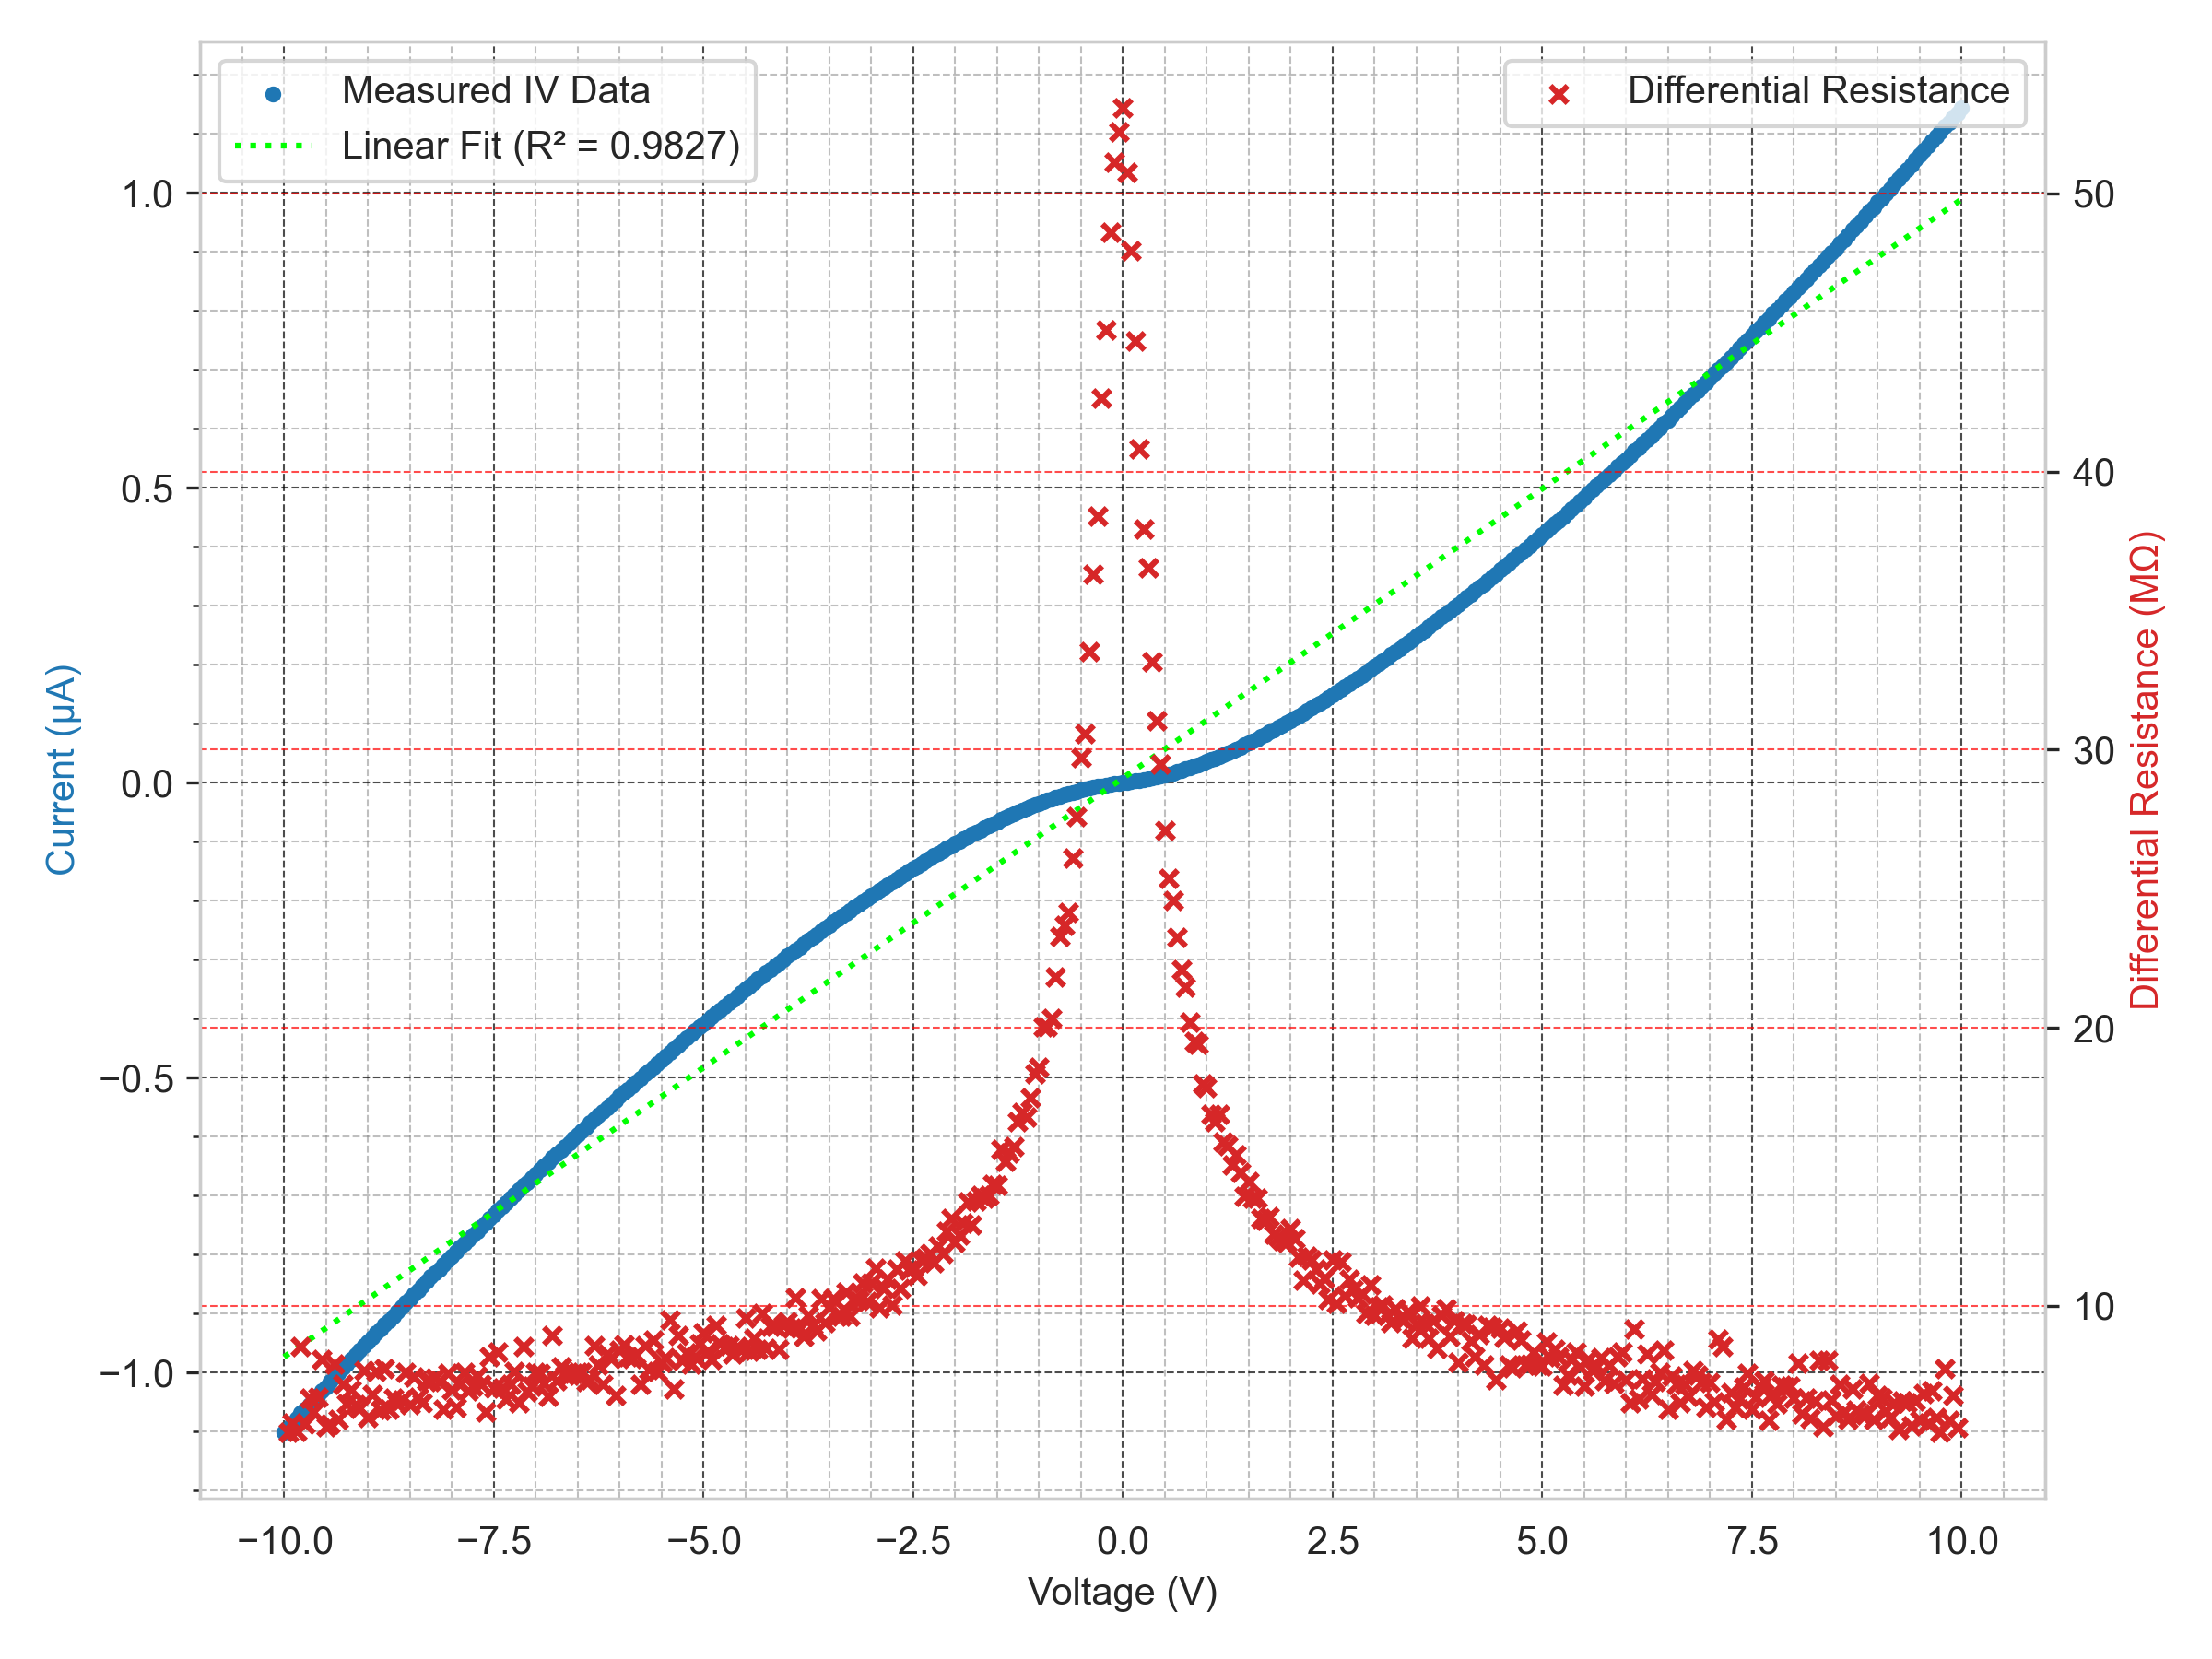
\includegraphics[width=\linewidth]{Chapter7/Figs/Raster/10V 13 d.png}
    \caption{The first electrical characteristics between probe positions 1 and 3.}
    \label{fig:10v_13}
\end{figure}

Figure \ref{fig:10v_13} shows the first measured IV characteristics of the 10~\si{\micro\metre} wire between probe positions 1 and 3. Of particular importance is the reduced absolute current relative to the thicker wire measurements, and also the clear Schottky behaviour, even given the lower bias range applied in this case. It was unclear initially if this behaviour was due to the wire itself at this stage in the experimental process. The differential resistance as plotted reflects this rise in Schottky behaviour at low voltages.

\begin{table}[ht]
\centering
\begin{tabular}{|c|c|c|c|}
\hline
Voltage (V) & Resistivity ($\Omega$m) & Conductivity (S/m) & Conductivity Error (S/m) \\
\hline
2 & $0.796$ & $1.25$ & $0.0895$ \\
10 & $0.364$ & $2.75$ & $0.196$ \\
\hline
\end{tabular}
\caption{Resistivity, conductivity, and errors for the wire between probes 1 and 3.}
\label{table:13_resistivity_conductivity_updated}
\end{table}

Table \ref{table:13_resistivity_conductivity_updated} provides a summary of the relevant conductivity data for the laser written wire between probe positions 1 and 3. The 10~\si{\volt} conductivity of approximately $2.75\pm0.20$~\si{\micro\metre} is significantly lower than the final 14~\si{\micro\metre} value of $28.5\pm1.7$~\si{\siemens\per\metre}.

\begin{figure}[H]
    \centering
    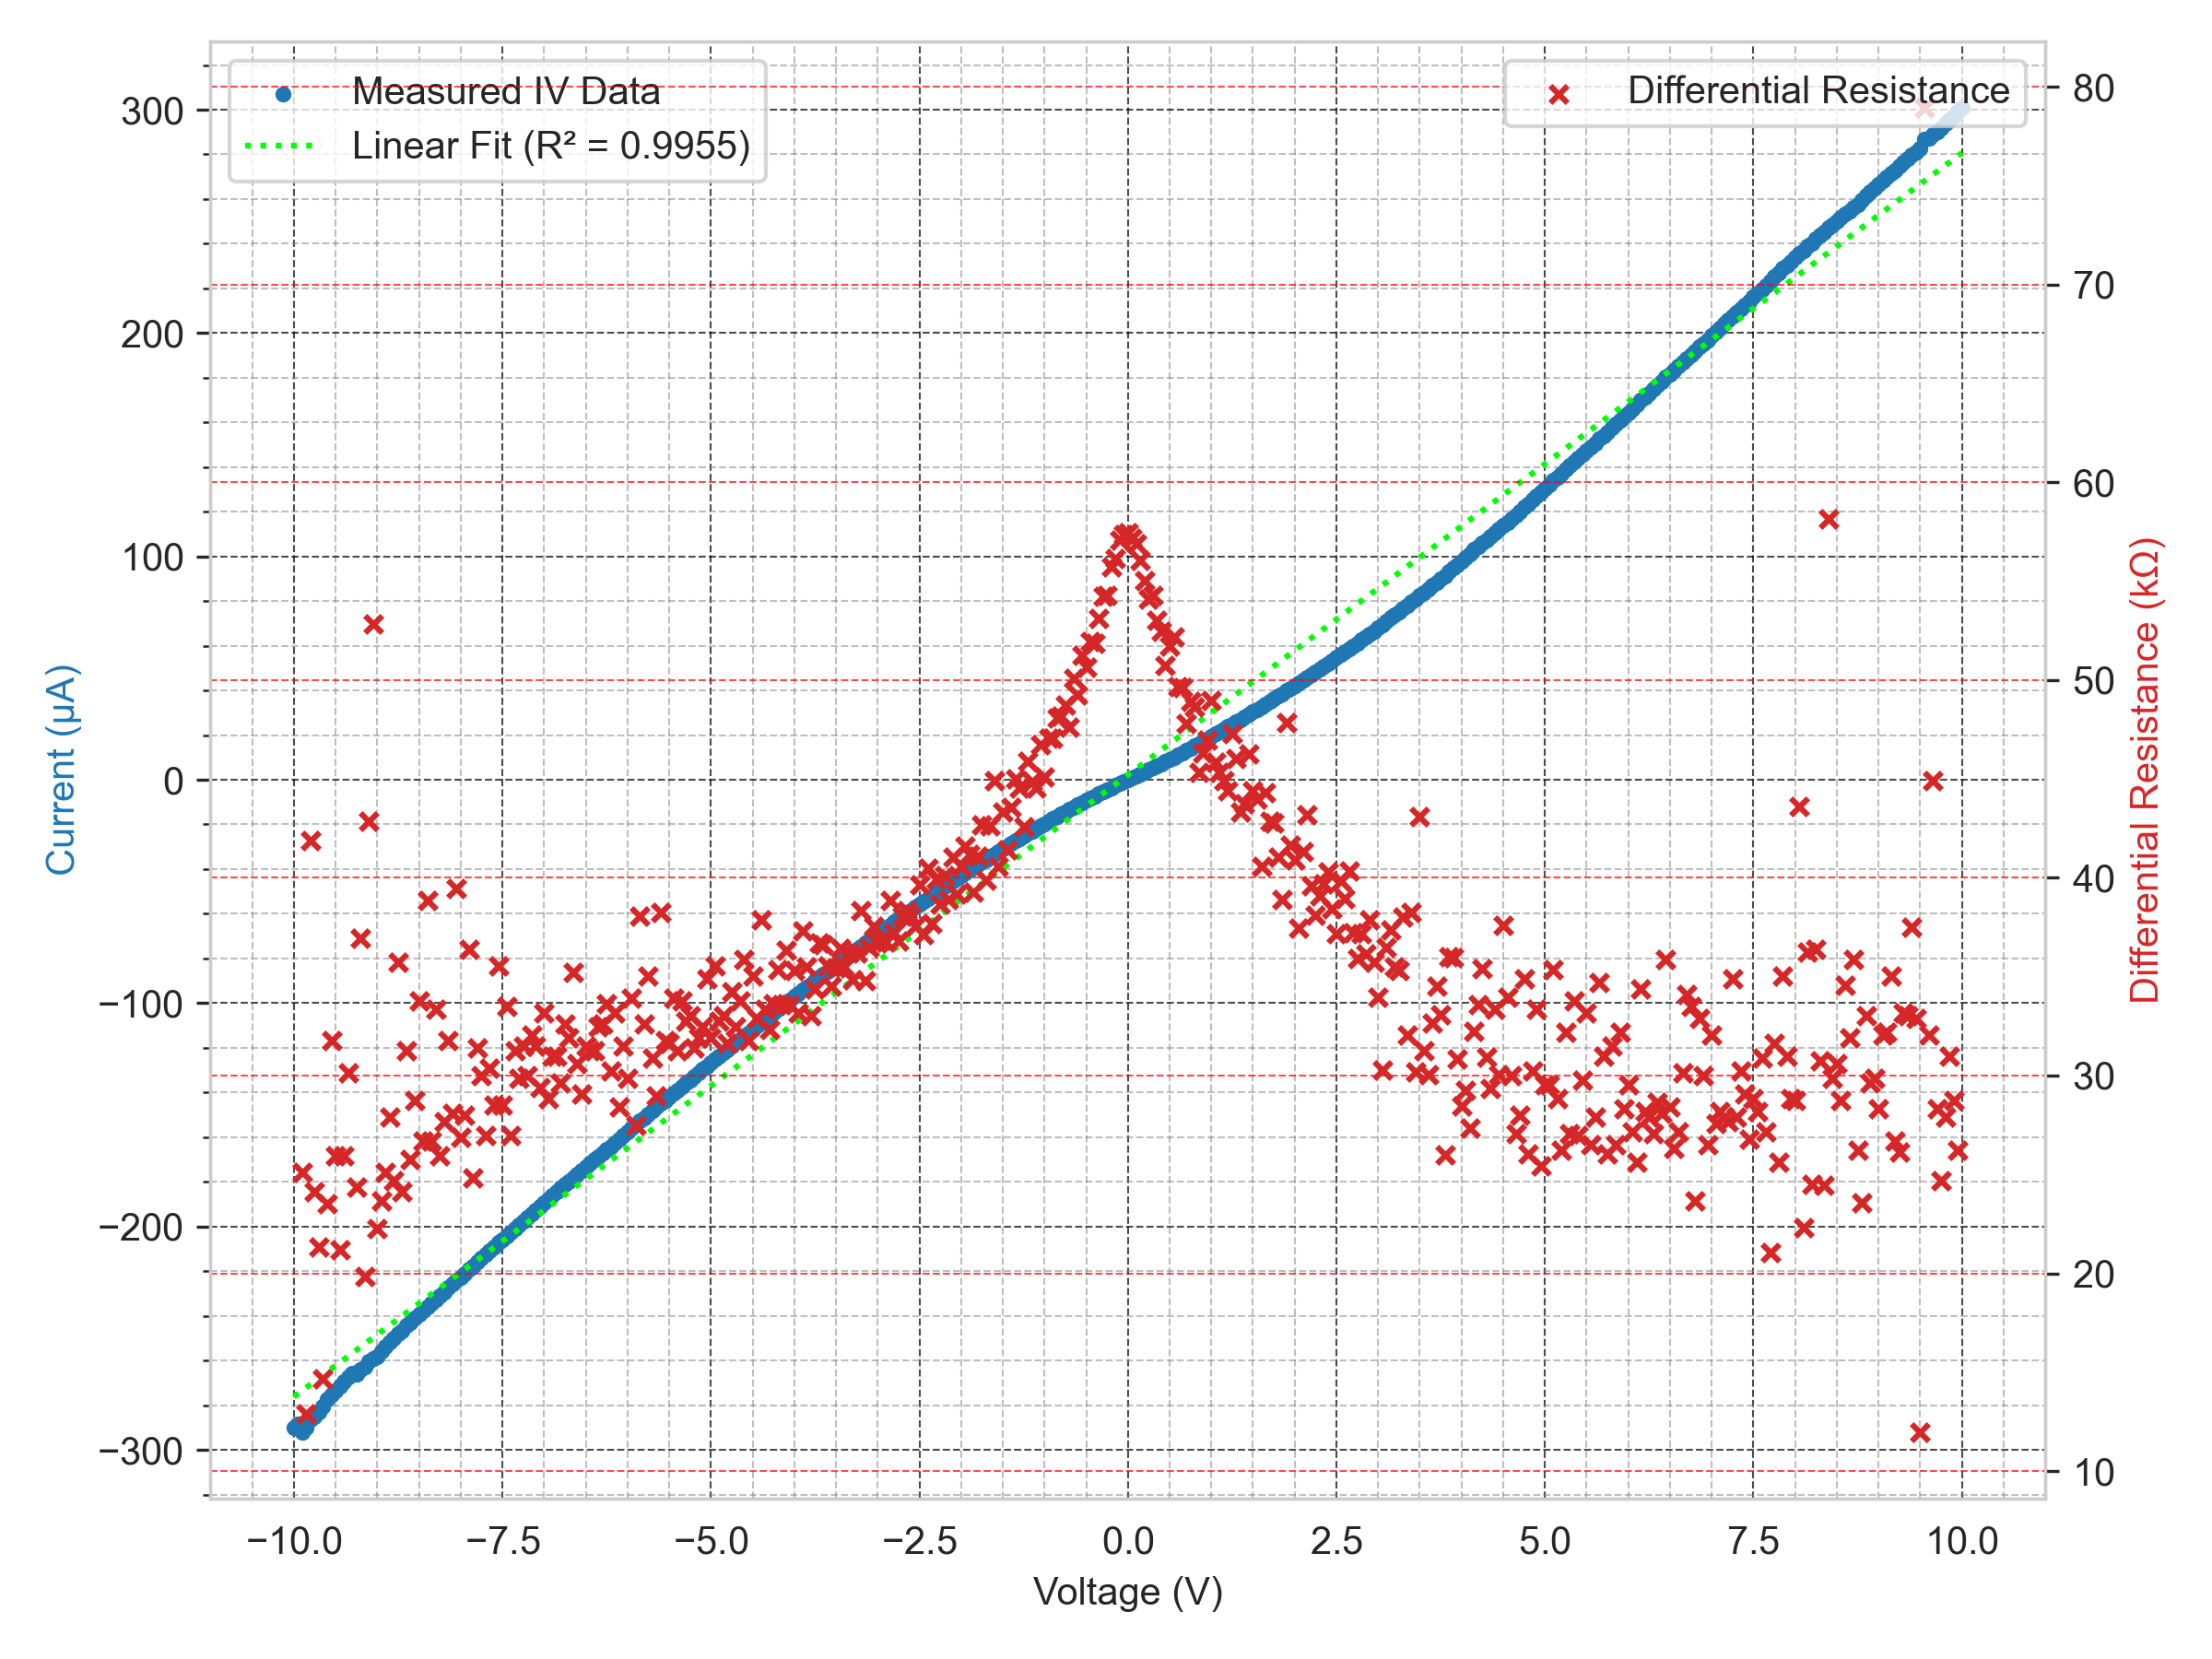
\includegraphics[width=\linewidth]{Chapter7/Figs/Raster/10V 24 d.png}
    \caption{The average electrical characteristics between probe positions 2 and 4.}
    \label{fig:10v_24}
\end{figure}

In figure \ref{fig:10v_24}, the IV measurements between probe positions 2 and 4 are plotted. This wire showed a significant jump in absolute current measurements, with the peak current reaching approximately $300$~\si{\micro\ampere}, in stark contrast to the previous measurements on both the comparable 1-3 wire and also the measurements across the 14~\si{\micro\metre}. The associated differential resistance is similarly lower by a few orders of magnitude.

\begin{table}[ht]
\centering
\begin{tabular}{|c|c|c|c|}
\hline
Voltage (V) & Resistivity ($\Omega$cm) & Conductivity (S/m) & Conductivity Error (S/m) \\
\hline
2 & 0.203 & 492 & 35.1 \\
10 & 0.128 & 780 & 55.7 \\
\hline
\end{tabular}
\caption{Resistivity, conductivity, and errors for the wire between probes 2 and 4.}
\label{table:24_resistivity_conductivity_updated}
\end{table}

In the same style as for the previous table of results for the wire between probes 1 and 3, table \ref{table:24_resistivity_conductivity_updated} shows the conductivity data for the 10~\si{\micro\metre} wire between probes 2 and 4. At 10~\si{\volt} the conductivity of this wire was measured to be approximately $780\pm1.3$~\si{\siemens\per\metre}, a factor of 284 increase in conductivity over the previous wire. This is also markedly higher than that of the 14~\si{\micro\metre} wire, with a factor of 27 increase in conductivity (for conductivity taken at 10~\si{\volt} in the 14~\si{\micro\metre} wire).

Following these results, it was apparent that repetition of the electrical characterisation was a necessity, as the drastic change in conductivity between different probe locations indicated that there may be some issues with making direct contact to the as processed laser written wires. Hence, the experimental procedure was repeated, with fresh probe tips and great care to ensure that the probe locations were as centrally located as physically possible to maximise the contacts formed. Several measurements performed with all 4 possible combinations of probe locations indicated that probe 3 in particular was the issue with the previous measurements.

\begin{figure}[H]
    \centering
    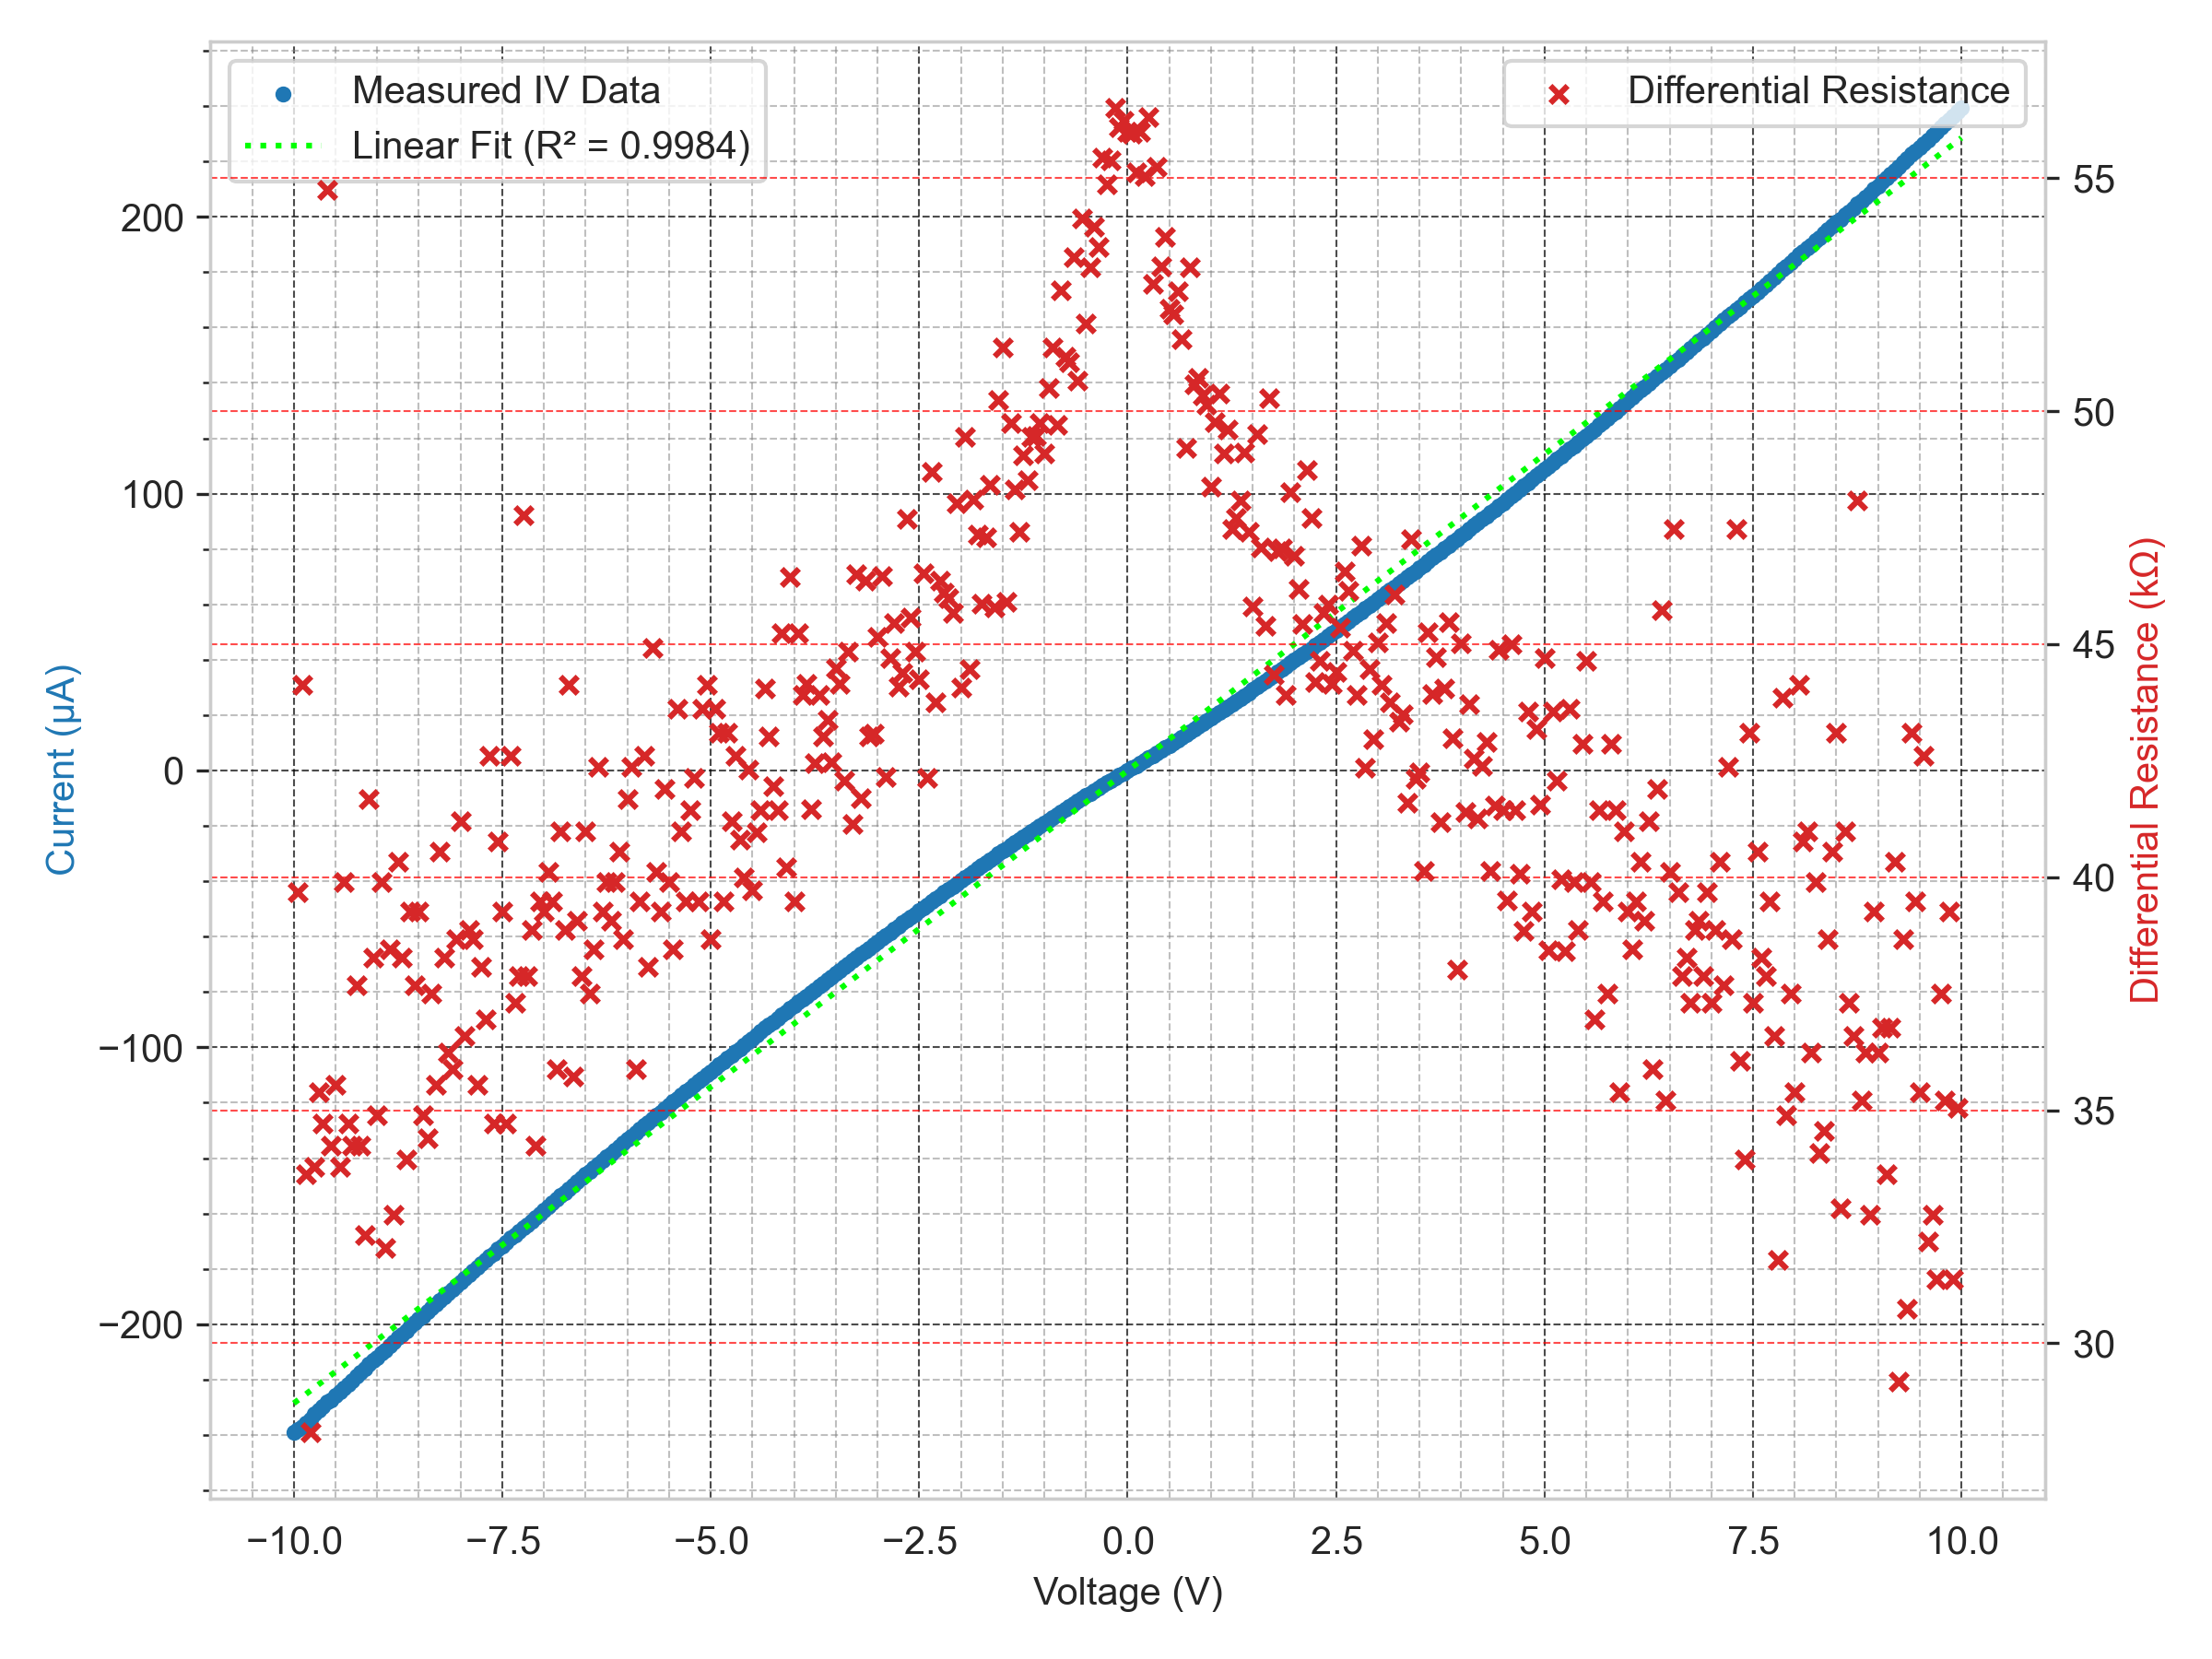
\includegraphics[width=\linewidth]{Chapter7/Figs/Raster/10V 13 replaced d.png}
    \caption{The average electrical characteristics between probe positions 1 and 3 - repeated.}
    \label{fig:10v_13_replaced}
\end{figure}

Figure \ref{fig:10v_13_replaced} shows the results of repeating this experiment with fresh probe tips and having had another standard solvent clean prior to making contact. The characteristics when contrasted to the previous data shown in figure \ref{fig:10v_13} are significantly more ohmic in nature, with the linear fit of R$^{2}$ value 0.9984 vs the previous fit of 0.9827 providing some quantification of this trend. As for 

\begin{table}[ht]
\centering
\begin{tabular}{|c|c|c|c|}
\hline
Voltage (V) & Resistivity ($\Omega$cm) & Conductivity (S/m) & Conductivity Error (S/m) \\
\hline
2 & 0.223 & 449 & 32.1 \\
10 & 0.156 & 640 & 45.7 \\
\hline
\end{tabular}
\caption{Resistivity, conductivity, and errors for the wire between probes 1 and 3 - repeated.}
\label{table:13_resistivity_conductivity_replaced}
\end{table}

The summary of further electrical measurements between probes 1 and 3 is given in table \ref{table:13_resistivity_conductivity_replaced}. Measurements between all 4 replaced probes were performed to confirm that none of the probes had a defective contact in this experimental setup, and the wire between positions 2 and 4 showed a similar conductivity to the previous results, at $749\pm53.5$~\si{\siemens\per\metre}. Further to this, a final complete replacement of electrical probes was performed to verify the order of magnitude of current being reported here, and this was in agreement. Therefore, it was concluded that the contacts in this setup were no longer the cause of any discrepancy between the measured wire conductivities. 

\subsection{Conductive Wire Testing - 10 and 14 microns}
\label{subsubsec:graphitised_wire_testing_both}
In the previous two sections, the experiments performed on the wire testing structure as shown in figure \ref{fig:big_bone_esid} were used to establish the observed electrical conductivities of the 10 and 14~\si{\micro\metre} wires. Several further sets of measurements were taken across the structure, as previously alluded to in the verification that the original contact formed by probe 3 was relatively poor compared to the other 3 points of electrical contact. While the measurements across the full span of the structure are more difficult to use for precise calculation of the effective conductivities involved due to the two differing wire widths, the observations thus far point to the thicker 14~\si{\micro\metre} wire having a conductivity approximately 30 times lower than that of the 10~\si{\micro\metre} wires. Hence, it is reasonable to assume that when electrical measurements are taken across the full span of the testing structure (such as between probes 1-2, 1-4 and 3-2, 3-4), the dominant resistance will likely be that of the 14~\si{\micro\metre} wire, despite the additional 10~\si{\micro\metre} wire paths.

\begin{figure}[H]
    \centering
    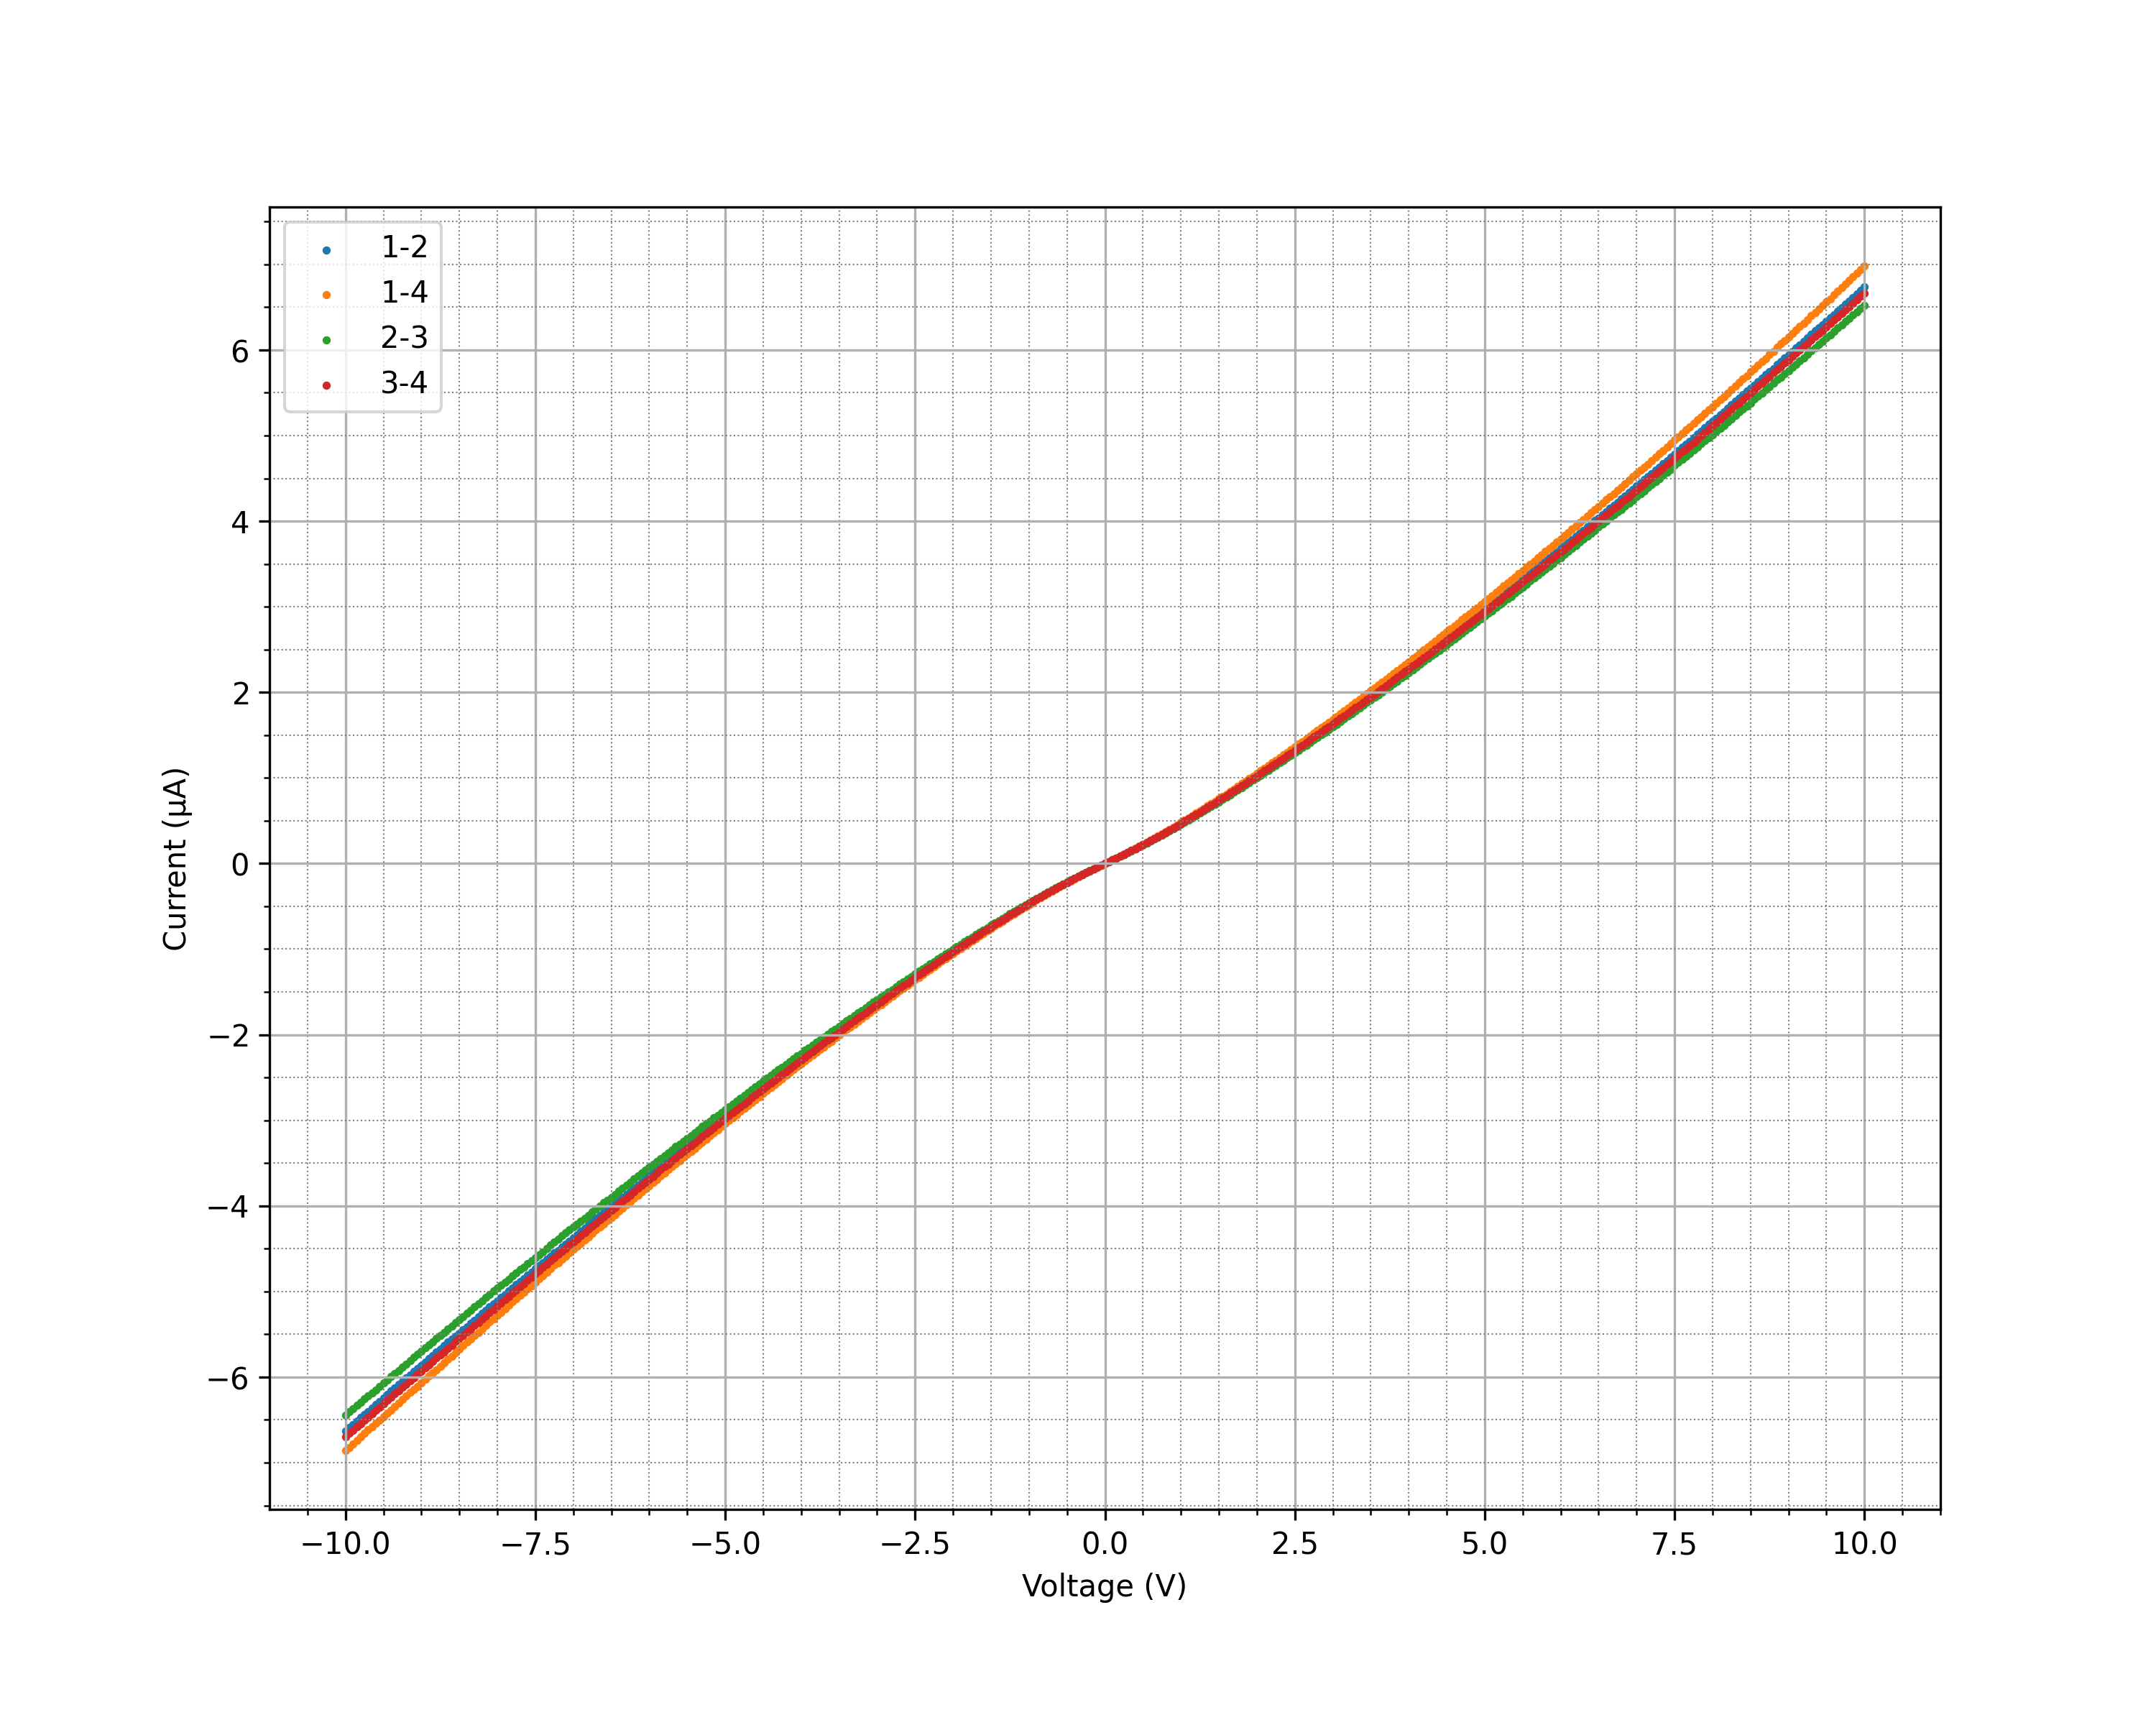
\includegraphics[width=\linewidth]{Chapter7/Figs/Raster/cross iv.png}
    \caption{The average IV characteristics across all four possible paths utilising the full wire test structure.}
    \label{fig:10v_big_bone}
\end{figure}

Figure \ref{fig:10v_big_bone} shows the overlay of all four differing sets of electrical measurements taken across the 14~\si{\micro\metre} wire via probes located on the 10~\si{\micro\metre} wires. It is difficult to see the dataset corresponding to the IV data between probes 1-2, as it very tightly follows the data for probes 3-4. Otherwise, there are only minor differences in the measured conductivities between these locations on the wire structure, and all four sets of measurements are in good agreement, despite the slight differences in wire lengths (1-2 $\sim295$~\si{\micro\metre}, 1-4/2-3 $\sim301$~\si{\micro\metre}, 3-4 $\sim305$~\si{\micro\metre}).

\begin{figure}[H]
    \centering
    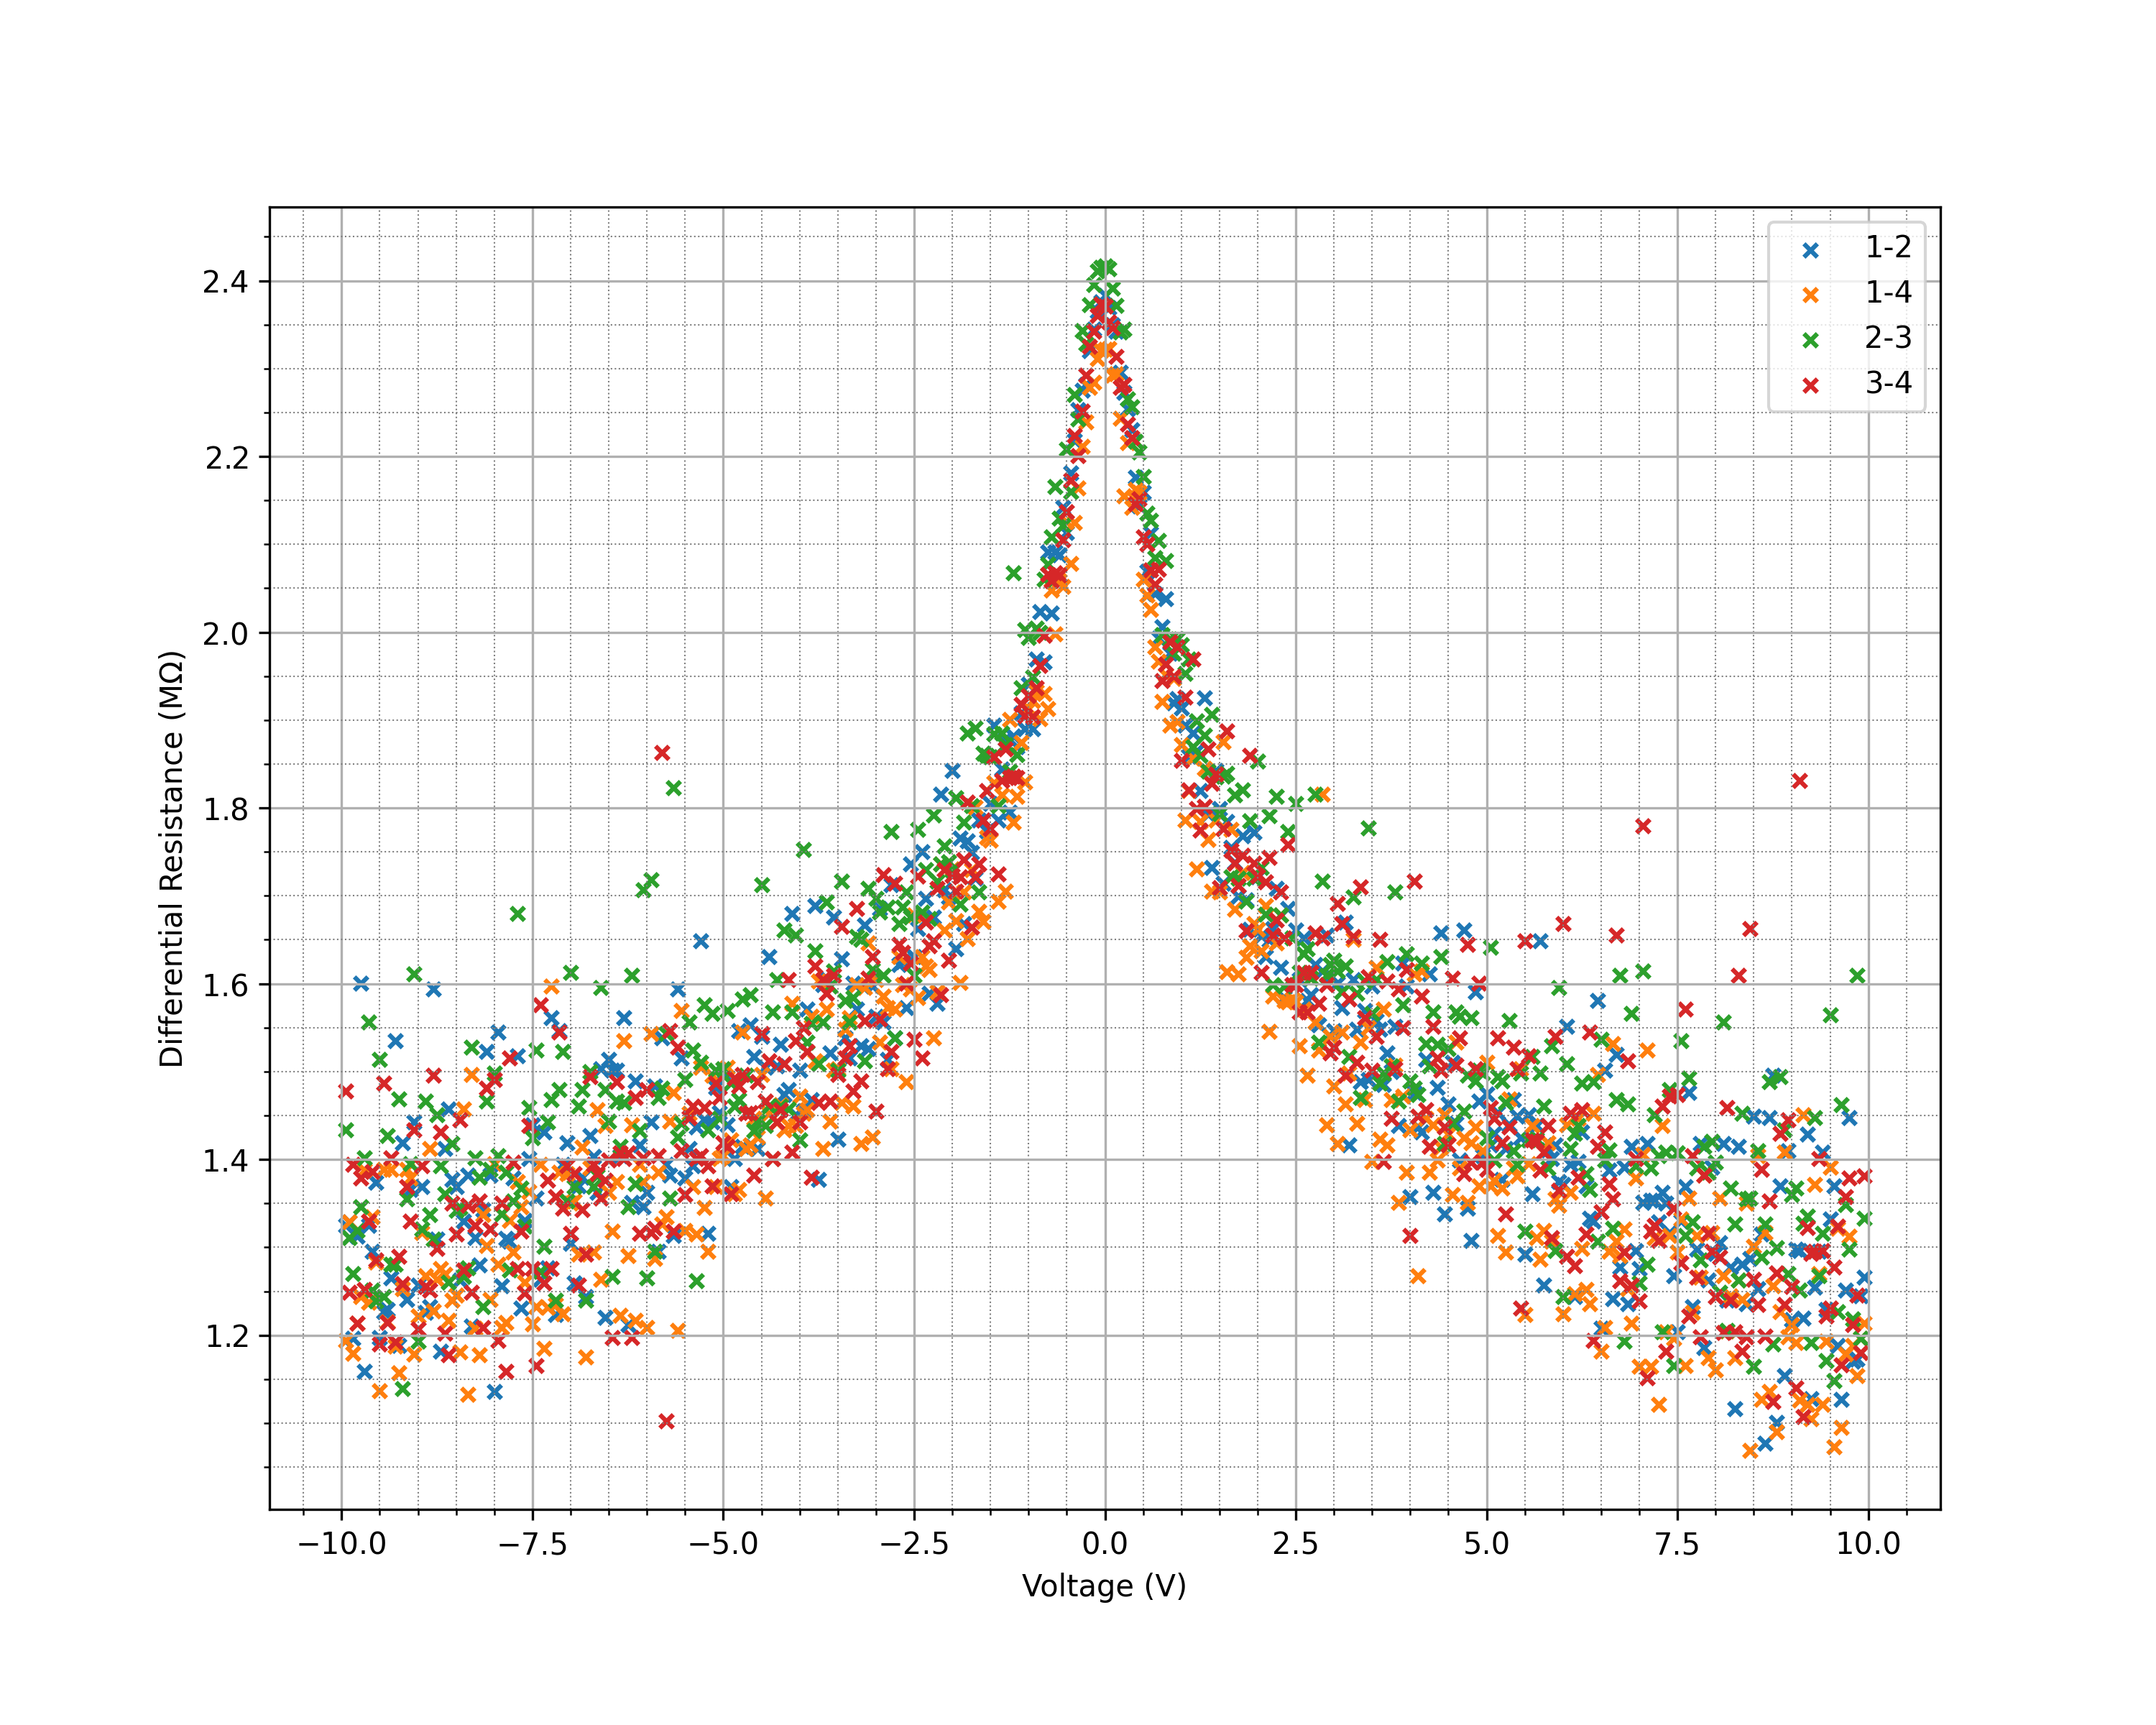
\includegraphics[width=\linewidth]{Chapter7/Figs/Raster/cross dr.png}
    \caption{The average differential resistance across all four possible paths utilising the full wire test structure.}
    \label{fig:10v_big_bone_dr}
\end{figure}

Figure \ref{fig:10v_big_bone_dr} shows an overlay of all four differential resistance plots across the test structure. Similar to the observations in figure \ref{fig:10v_big_bone}, the electrical characteristics are consistent across all paths. However, at higher voltages, a notable spread in differential resistance values is observed. This variability might be attributed to the differing number of data points per sweep, with 1000 data points typically collected in most sweeps, and a minimum of 400 in others. More consistent sampling across sweeps, and increasing the number of data points, is likely to enhance the precision and reduce the variability of the results. Each IV sweep was performed three times, spaced by a minimum of 10 seconds between each sweep to mitigate any effects of residual charge build-up, ensuring that the measurements reflect the true resistance of the wire without interference from transient electrical effects.

\begin{table}[ht]
\centering
\begin{tabular}{|c|c|c|c|c|}
\hline
Path & Resistance (M$\Omega$) & Resistivity ($\Omega$cm) & Conductivity (S/m) & Error (S/m) \\
\hline
1-2 & $1.58$ & $3.21$ & $31.1$ & $2.22$ \\
1-4 & $1.53$ & $3.05$ & $32.7$ & $2.34$ \\
3-2 & $1.63$ & $3.25$ & $30.8$ & $1.06$ \\
3-4 & $1.58$ & $3.11$ & $32.2$ & $1.09$ \\
\hline
A-B & $0.992$ & $4.24$ & $23.6$ & $1.44$ \\
1-3 & $0.0438$ & $0.156$ & $640$ & $45.7$ \\
2-4 & $0.0370$ & $0.132$ & $756$ & $54.0$ \\
\hline
\end{tabular}
\caption{Summary of electrical measurements at 10~\si{\volt} for different probe configurations.}
\label{table:electrical_measurements_10v_all}
\end{table}

In table \ref{table:electrical_measurements_10v_all}, the various electrical measurements across all four different "cross" configurations. Note that the calculation of resistivity and hence conductivity in this table uses an average wire width of 12~\si{\micro\metre} (in the first half), to provide an estimate for comparison with previous measurements across single wires. These measurements can be interpreted as three separate resistors in series, utilising wires that were characterised individually in the lower half of the table. All four electrical paths showed a reasonable similarity, with the potential error due to probe positioning potentially negating the slight differences observed. The lower half of the table provides the final measurements for each individual wire section, which highlights again the dominance of the resistance caused by the 14~\si{\micro\metre} wire.

\begin{figure}[H]
    \centering
    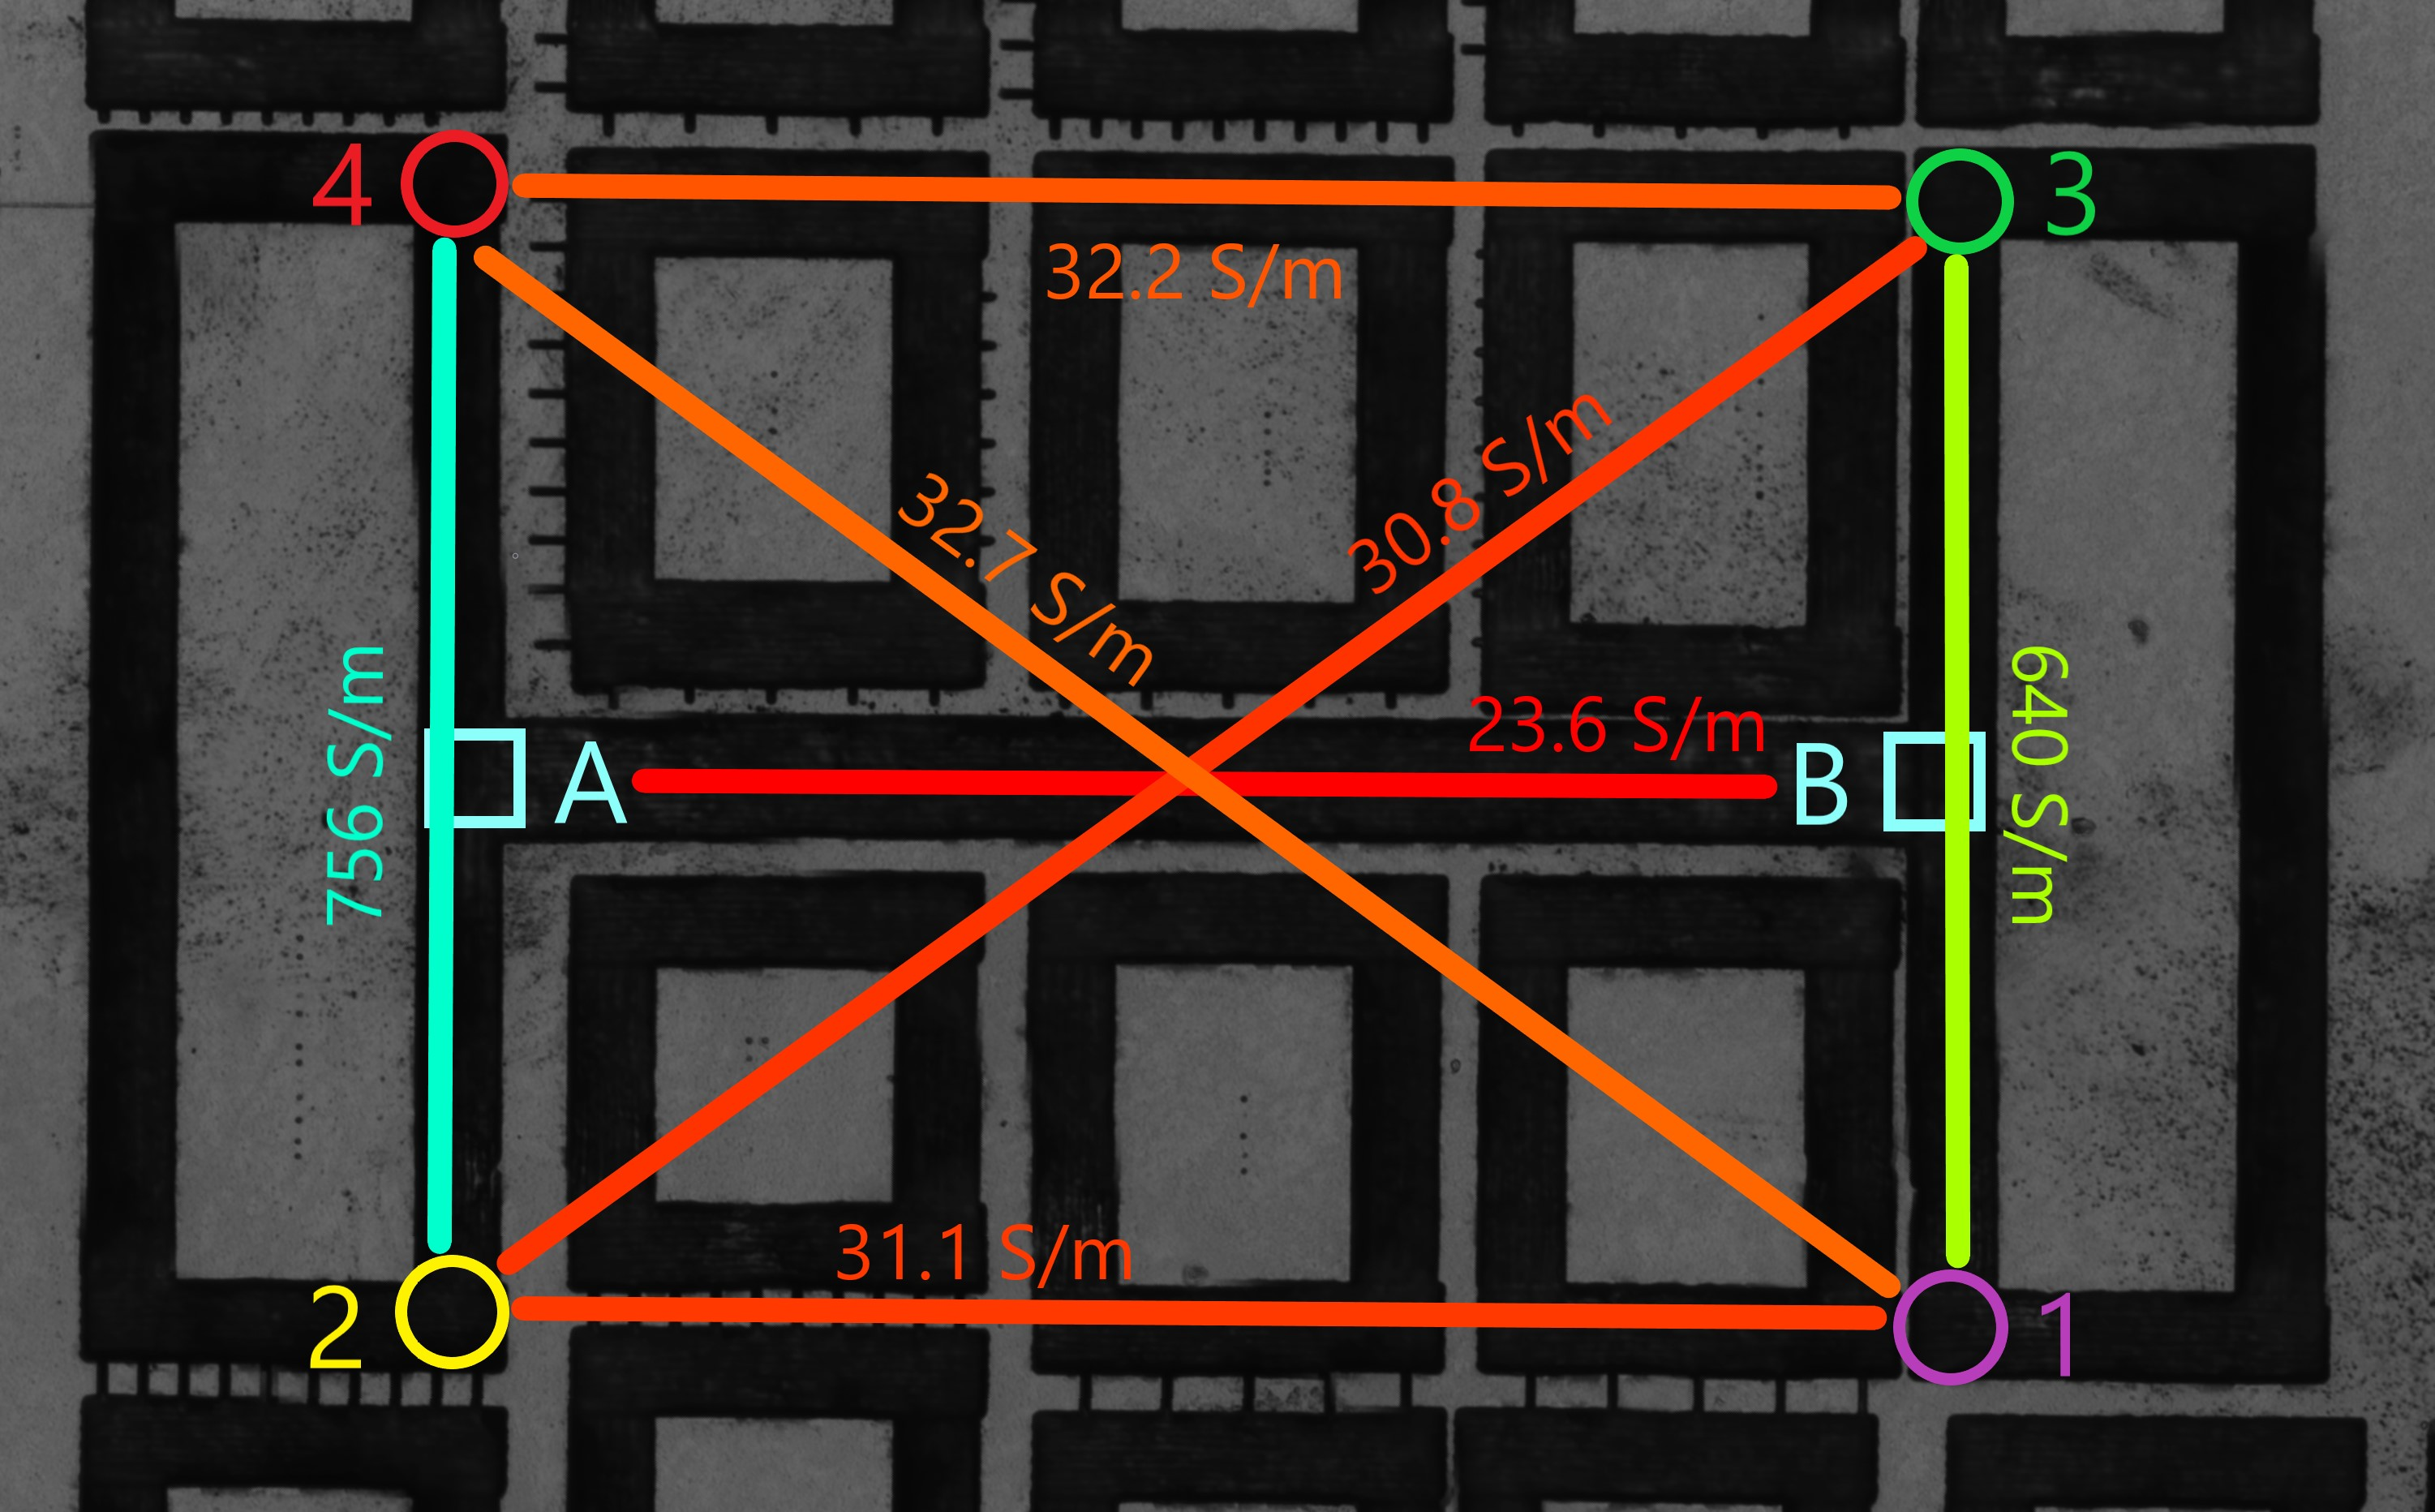
\includegraphics[width=\linewidth]{Chapter7/Figs/Raster/big_bone_esid_annotated_2.jpg}
    \caption{A simplified summary of the electrical characterisation of wire structures, as observed at 10~\si{\volt}.}
    \label{fig:big_bone_esid_2}
\end{figure}

Figure \ref{fig:big_bone_esid_2} provides a visual representation of the electrical measurements performed to determine the effectiveness of laser writing in creating ohmic wire structures. A colour spectrum is used with the simplified straight line connections to show the relative conductivities for the differing paths. The most noteworthy conclusion from these measurements was that the 10~\si{\micro\metre} wires were not merely ohmic, but were in fact significantly more ohmic than what was presumed to be the most electrically conductive structure in the design (the 14~\si{\micro\metre} wide wire). While there are some slight differences in the conductive paths that utilise both the cross bar and the thinner wires, the differences are not significant enough with the error analysis to conclude that any particular parts of the wires were more or less conductive. This is represented by the slight shift from red-orange that is present in the straight line connections used to represent these electrical paths. The only clear difference was between the two 10~\si{\micro\metre} wires, which showed an 18\% conductivity improvement in the leftmost wire between points 4-2, when compared to the rightmost wire between points 3-1.

\subsection{Comparison to Graphite}
\label{subsubsec:comparison_to_graphite}
With the measured conductivities following a number of assumptions regarding the geometric properties of the laser written wires, it is now a reasonable step to compare these values to what might be expected from ideal graphite wires. Then, it is possible to ask what the geometry of these graphite wires must be to match the measured resistances. It is inferred that the thickness of such a pure graphite wire must follow:
\begin{equation}
    t = \frac{L}{\sigma RW}
    \label{eq:thickness_conductivity}
\end{equation}

Using a low estimate of the basal plane conductivity for typical graphite ($\sim2\times10^{5}~\si{\siemens\per\metre}$ \cite{pierson1993}, and by comparing to the measured resistance for the highest calculated conductivity of $756$~\si{\siemens\per\metre} (path 2-4, as outlined in table \ref{table:electrical_measurements_10v_all}), the effective thickness of such an ideal wire is calculated to be $1.89$~\si{\nano\metre} in thickness. While the inter-atomic spacing between graphene sheets within graphite is a strong function of temperature and also depends upon the stacking sequence, typical inter-layer spacings are of the order of $0.355$~\si{\nano\metre} \cite{pierson1993}. Hence, a low estimate of basal plane conductivity for ideal graphite indicates an effective wire of only $\sim5$ layers of thickness.

If instead, conduction is considered perpendicular to the basal plane of $\sim300$~\si{\siemens\per\metre} \cite{pierson1993}, and again the highest calculated conductivity wire is used as a resistance reference point, the effective thickness of this wire is calculated to be $1.26$~\si{\micro\metre}. This is not too surprising, since the assumption of thickness $0.5$~\si{\micro\metre} was used in the calculation of conductivity $756$~\si{\siemens\per\metre} for this wire originally. It does however confirm that for the electrical characteristics as performed on the 10~\si{\micro\metre} wide wires, graphite-like conductivity over a wire thickness that is reasonable does appear to be observed. Indeed the conductivity is more than 2 times higher when it is assumed that the thickness is $0.5$~\si{\micro\metre}, which as discussed in section \ref{subsubsec:laser_writing_thickness} represents a fair estimate based on literature values. Much thicker than $1$~\si{\micro\metre} is unlikely, though further studies on laser graphitisation of diamond may help to elucidate the mechanisms determining the depth at which conductive material is generated, be that in the form of graphitic, diaphitic, or segregated areas of sp$^{2}$ bonding in a percolative network, as well as the interplay between these materials in conductors.

Finally, for the case of lower conductivity, such as that for the wire between points A-B, considering graphitic conduction perpendicular to the basal plane of $\sim300$\si{\siemens\per\metre} \cite{pierson1993}, the effective thickness for the measured resistance is $39.4$\si{\nano\metre}. It is certainly possible that the assumption of relatively uniform graphitised material may be significantly incorrect in this wire, with some narrow conductive paths leading to the observed resistance. However, this is at least mildly odd, implying that despite the wire being significantly wider, the conductive path formed is substantially more inconsistent in thickness to the degree that the additional width is irrelevant. This is perhaps another indicator that the conductive material formed by this process cannot be simply regarded as "graphitic", despite the successful application of such a descriptor to the thinner wires. Instead, it must be considered that such conduction is due to electrical percolation and nanostructure assemblies as described by complex network theory \cite{mclachlan1990, yao2020}. Broken type 2 diaphite is another likely contender in such poorly conducting material, with recent work examining the shift between ohmic and semiconducting material due to differing laser parameters highlighting the potential for such broken conductive paths to transition from ohmic type 1 diaphite wires to highly resistive type 2 diaphite wires \cite{salter2024}.

Usage of the low estimated conductivity for in-plane graphite leads to an effective thickness of $59$~\si{\pico\metre} when the values for path A-B are used again, around 7 times thinner than that of typical measured thicknesses of single graphene layers \cite{shearer2016}. This provides further confirmation that on the scale from a thin highly conductive layer of sp${2}$ bonded carbon, to very thick, poorly conducting amorphous carbon containing sp$^{2}$ bonding, it must necessarily be well away from the edge case of a single graphene layer providing the bulk of observed conductivity. It is impossible to rule out a "broken islands" structure of graphene conductivity, but this is again leading to a complex network theory or electrical percolation model. In which case, it is more likely that layers of graphene are not the cause of conductivity.

Regardless of the exact geometric and material model underlying the observed conductive paths, these conductive paths are sufficient to provide electrical wires embedded within the diamond surface. The contact between such wires and the phosphorous doped diamond surface layer may now be considered.

\section{LTLM Structure}

\begin{figure}[H]
    \centering
    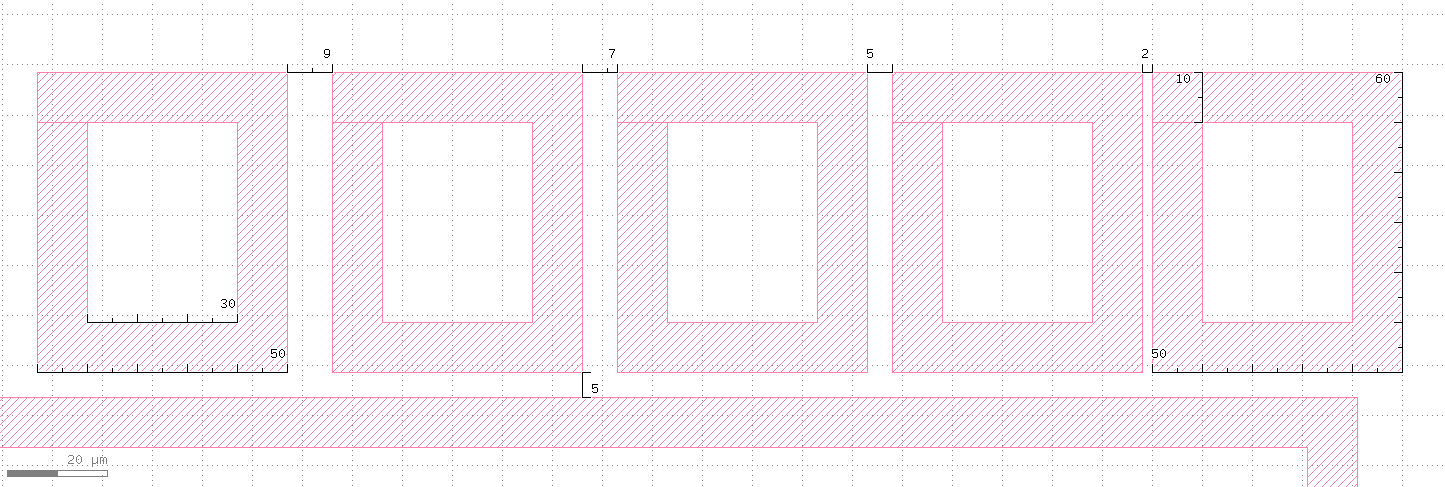
\includegraphics[width=\linewidth]{Chapter7/Figs/Raster/ltlm_design.png}
    \caption{The design of a LTLM structure for laser processing.}
    \label{fig:ltlm_design}
\end{figure}

As established in section \ref{subsubsec:comparison_to_graphite}, the electrical conductivity of the wires is sufficient to proceed with testing of diamond devices manufactured with these wires. In particular, one of the intended device structures is that of emitters, or emitter arrays. However, before testing such devices, it is important to have a baseline of comparison, which in practical terms results in a simple LTLM structure, as that will provide a test of "emitter-less" devices. This has the additional benefit of providing a comparison to conventional Ti-based ohmic contacts, which rely on annealing to generate a TiC interlayer for the reduction of Schottky barrier height and the subsequent reduction in specific contact resistivity. Figure \ref{fig:ltlm_design} shows the designed structure of this LTLM-type setup. Four channel lengths between 2--9~\si{\micro\metre} are included, with simple rectangular wires providing the effective contacts. As shown in section \ref{subsec:afm_characterisation}, the channel width as measured via topological surveys shows some error in particular locations. It is important to examine these contacts prior to any LTLM analysis, due to the potential for significant deviation from the intended device structure.

\subsection{LTLM Microscopy}

\begin{figure}[H]
    \centering
    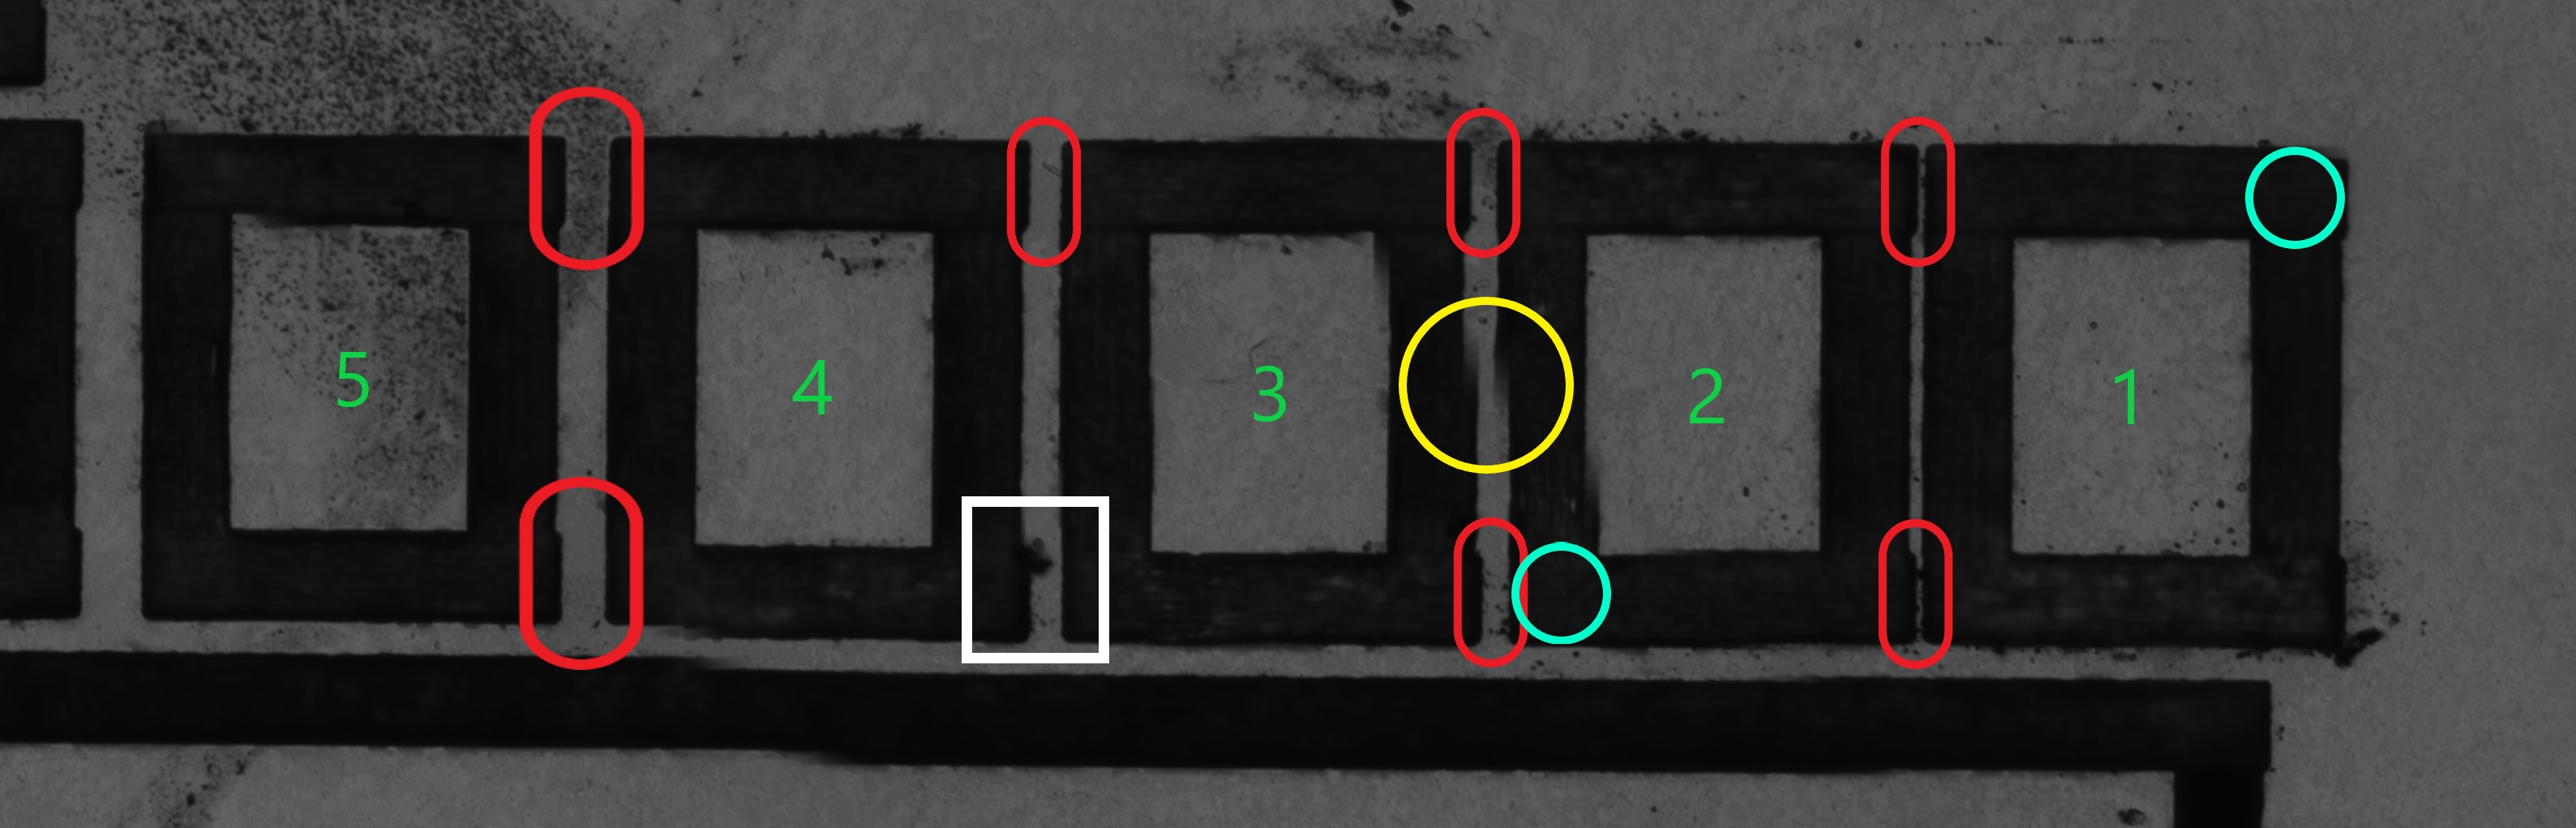
\includegraphics[width=\linewidth]{Chapter7/Figs/Raster/ltlm_esid_annotated4.jpg}
    \caption{The LTLM laser written structure as observed via confocal microscopy with a 488~\si{\nano\metre} light source. Annotated numbers indicate the contact label.}
    \label{fig:ltlm_esid}
\end{figure}

Figure \ref{fig:ltlm_esid} shows the laser processed device structure as seen via confocal microscopy, utilising a 488~\si{\nano\metre} back-light. The different electrical wires used to form effective contact regions are labelled 5--1 from left to right. Red capsules are used to highlight corners of the contacts where it appears that a slight overshoot relative to the vertical wires has occurred. In the case of the channel between contacts 2-1, this results in what appears to be a potential overlap at this scale between the contacts in laser written graphitic content. In the case of the other channels it simply produces a small region at the corners where visible narrowing occurs. The yellow circle indicates what appears to be a slight mismatch in the vertical wires at the edges of contact 3 and 2. On contact 3, the wire appears to fade away to transparent diamond moving upwards and out of this circle, while on contact 2 the wire at the edge of the contact appears to similarly fade into transparency moving downwards. The net result is a region in the centre of the circle in particular where the channel appears to have its narrowest point, and significantly wider regions before the corners. Finally a white square highlights what appears to be an amorphous blob on the bottom right corner of contact 4. It is unclear if this is due to the laser writing, or if it is contamination on the surface of the diamond. A region of small, soot-like contamination appears in various locations of this image, particularly near contact 5. It is possible that this is graphitic material due to ablation during the laser processing, which has not been removed in the subsequent solvent cleaning steps. Other possibilities, such as absorbance of the back-lighting within the substrate itself, may be considered via examination of other microscopy imaging utilising a top-down light source.

A final detail included in figure \ref{fig:ltlm_esid} is that of the cyan circles on contacts 2 and 1. These represent the two probe locations which were used for electrical characterisation across the 2~\si{\micro\metre} channel. Similar positions were used for the rest of the LTLM channels, with the right-most probe being located on the upper right corner of the contact structure and the left-most contact positioned on the lower left corner of the corresponding contact. This was done to ensure as much consistency as possible with the electrical measurements, as changing the relative positions of the probes on the contacts beween channels would change the resistance due to the 10~\si{\micro\metre} wire resistivity. As previously established, the 10~\si{\micro\metre} wires demonstrate the highest electrical conductivity, so the voltage drop across these wires should be minimal in comparison to the phosphorous doped diamond channel. However, this factor cannot be overlooked and is considered in the analysis of electrical measurements.

\begin{figure}[H]
    \centering
    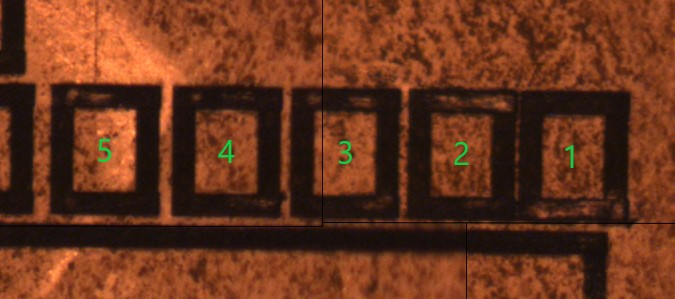
\includegraphics[width=\linewidth]{Chapter7/Figs/Raster/ltlm_afmm_annotated.jpg}
    \caption{The LTLM laser written structure as observed via optical microscopy with a white light source.}
    \label{fig:ltlm_afmm}
\end{figure}

Figure \ref{fig:ltlm_afmm} shows a tiled image of the LTLM structure, as seen with a standard optical microscope (air immersion). The resolution of this image is significantly lower than that of the back-lit microscopy shown in figure \ref{fig:ltlm_esid}, but it provides another visual comparison of the LTLM structure. In particular, the concentration of absorbent soot-like contamination near contact 5 is now visible as a reflective region on the surface of the sample, in contrast to the other areas which are not reflective.

\begin{figure}[H]
    \centering
    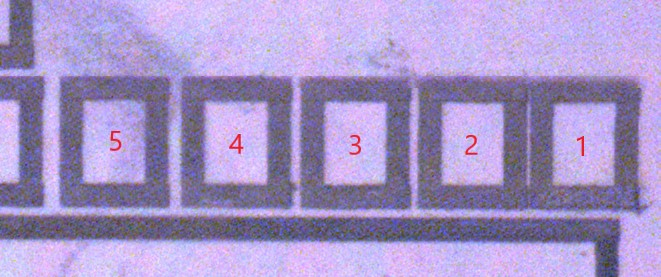
\includegraphics[width=\linewidth]{Chapter7/Figs/Raster/ltlm_afmm_dark_annotated.jpg}
    \caption{The LTLM laser written structure as observed via optical microscopy with a back-lit white light source.}
    \label{fig:ltlm_afmm_dark}
\end{figure}

Figure \ref{fig:ltlm_afmm_dark} provides a white back-lit image of the LTLM devices, using the same optical microscope as for the top-down white light source imaging in figure \ref{fig:ltlm_afmm}. Similar to that of the 488~\si{\nano\metre} back-lit confocal microscopy of figure \ref{fig:ltlm_esid}, the soot-like contamination around contact 5 is seen to absorb a fraction of the white light source. It is notable that in contrast to the complete absorption of 488~\si{\nano\metre} light, this region does appear to have some transparency in the visible light range. However, given the significant disparity in optical resolution with this image, it is still possible that these particles are strongly absorbing the full visible light range. Regardless, this provides further comparative optical imaging for a qualitative examination of the device structures.

\begin{figure}[H]
    \centering
    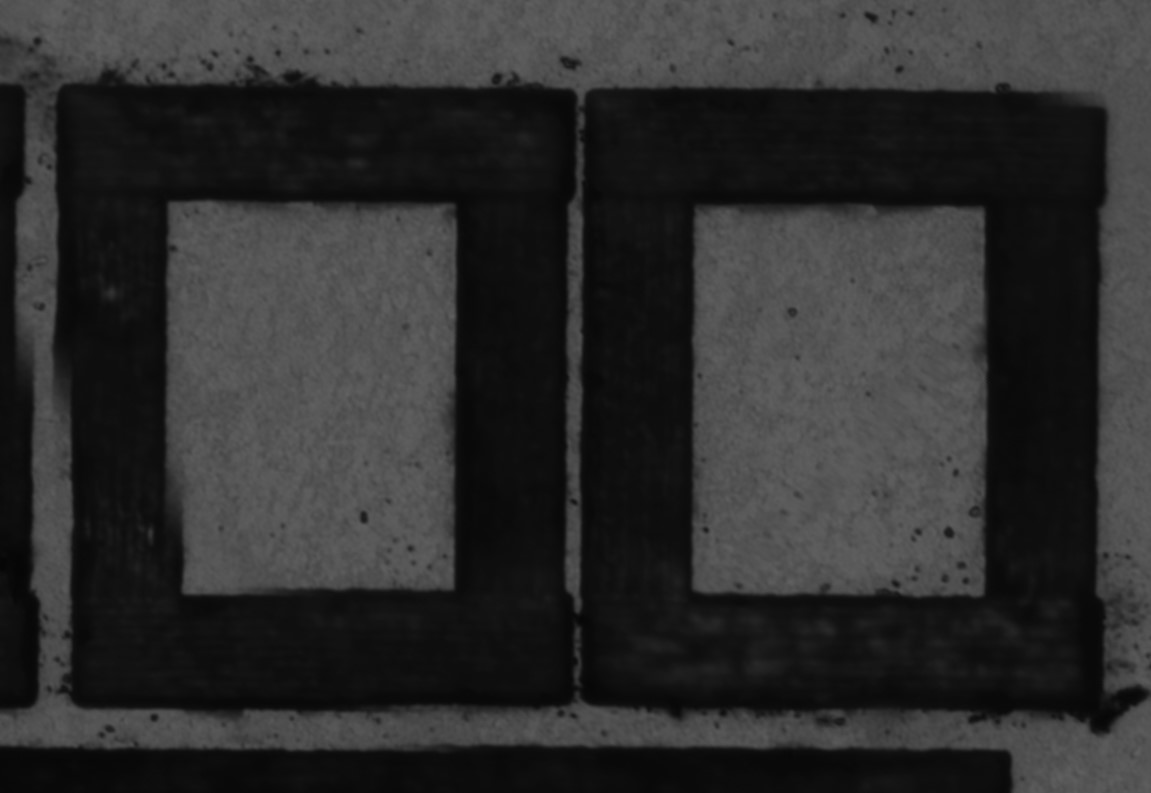
\includegraphics[width=\linewidth]{Chapter7/Figs/Raster/21_esid.jpg}
    \caption{Contacts 2-1 of the LTLM structure, more closely examined via 488~\si{\nano\metre} confocal microscopy.}
    \label{fig:21_esid}
\end{figure}

Figure \ref{fig:21_esid} provides a view of contacts 2-1, as viewed via 488~\si{\nano\metre} confocal microscopy. At this scale the limit due to diffraction is starting to become evident, since the estimated limit of spatial resolution for the oil-immersion confocal microscope used is 200~\si{\nano\metre} with the 488~\si{\nano\metre} laser used.

\begin{figure}[H]
    \centering
    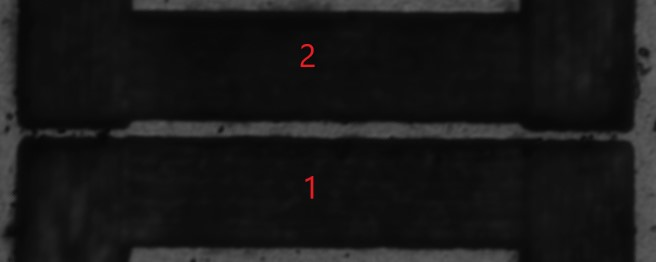
\includegraphics[width=\linewidth]{Chapter7/Figs/Raster/21 channel limit esid.jpg}
    \caption{Contacts 2-1 of the LTLM structure, at the optical limit via 488~\si{\nano\metre} confocal microscopy.}
    \label{fig:21_esid_closer}
\end{figure}

\begin{figure}[H]
    \centering
    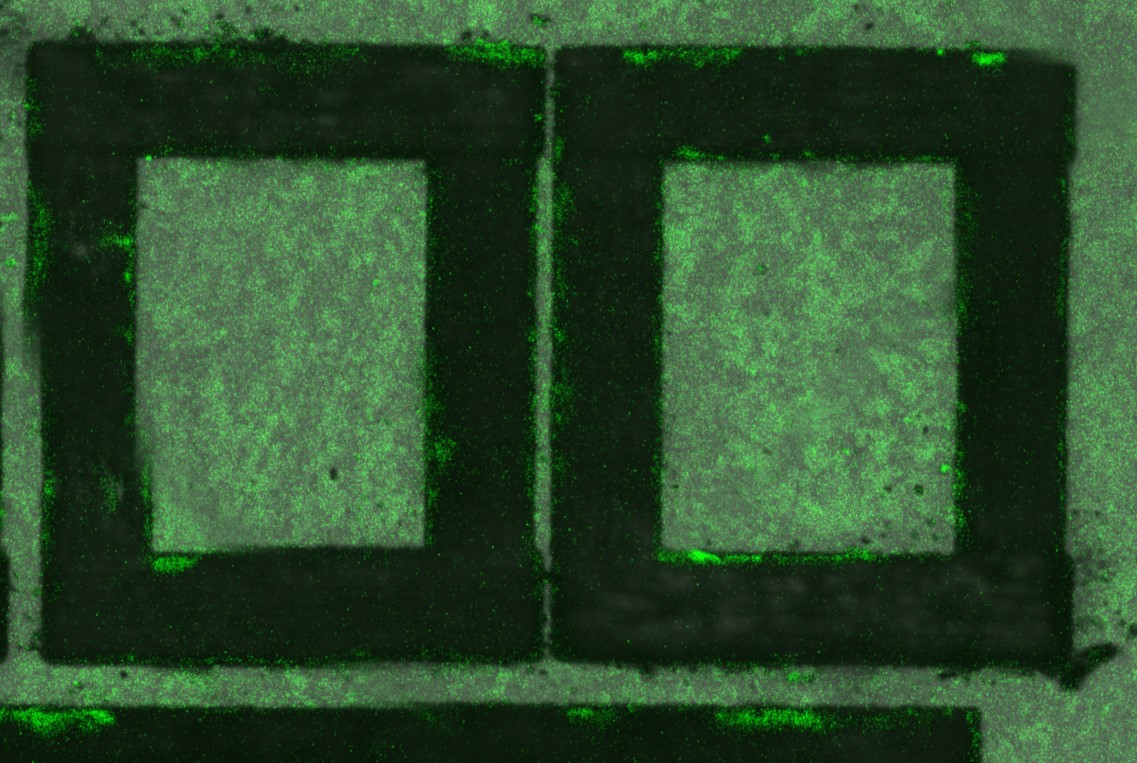
\includegraphics[width=\linewidth]{Chapter7/Figs/Raster/21_fl_esid.jpg}
    \caption{Contacts 2-1 of the LTLM structure, more closely examined via 488~\si{\nano\metre} confocal microscopy with 408~\si{\nano\metre} excited fluorescence.}
    \label{fig:21_fl_esid}
\end{figure}

In figure \ref{fig:21_fl_esid}, the fluorescence due to an excitation laser of 408~\si{\nano\metre} is overlaid onto the 488~\si{\nano\metre} confocal microscope imaging of figure \ref{fig:21_esid_closer}. While the source of any fluorescence is speculative, this provides another view of the laser written LTLM electrical contacts. 

One noteworthy conclusion that is drawn from these high spatial resolution optical images of the contacts is that the slight overshoot observed at the corners of each contact appears to be touching at the bottom of the channel between contacts 2-1. At minimum, the spatial resolution of 200~\si{\nano\metre} is insufficient to resolve a clear spacing between the contacts in this region. As has been previously discussed in this chapter, the exact composition of laser processed wires and the resulting electrical characteristics could vary quite widely. While there is a visual "short" between the two contacts, if the dark material seen in this region is highly resistive, then the effective channel width may well still approach that of the designed 2~\si{\micro\metre}. While electrical characteristics indicating an intact semiconducting channel will help to disprove the existence of any electrical short, it is important to consider that the material connecting these two contacts may still be a semiconducting allotrope of carbon, but it may no longer be that of highly phosphorous doped diamond. This may distort the results if it is less resistive than that of the diamond channel, but still appear as though it is a semiconducting channel.

\begin{figure}[H]
    \centering
    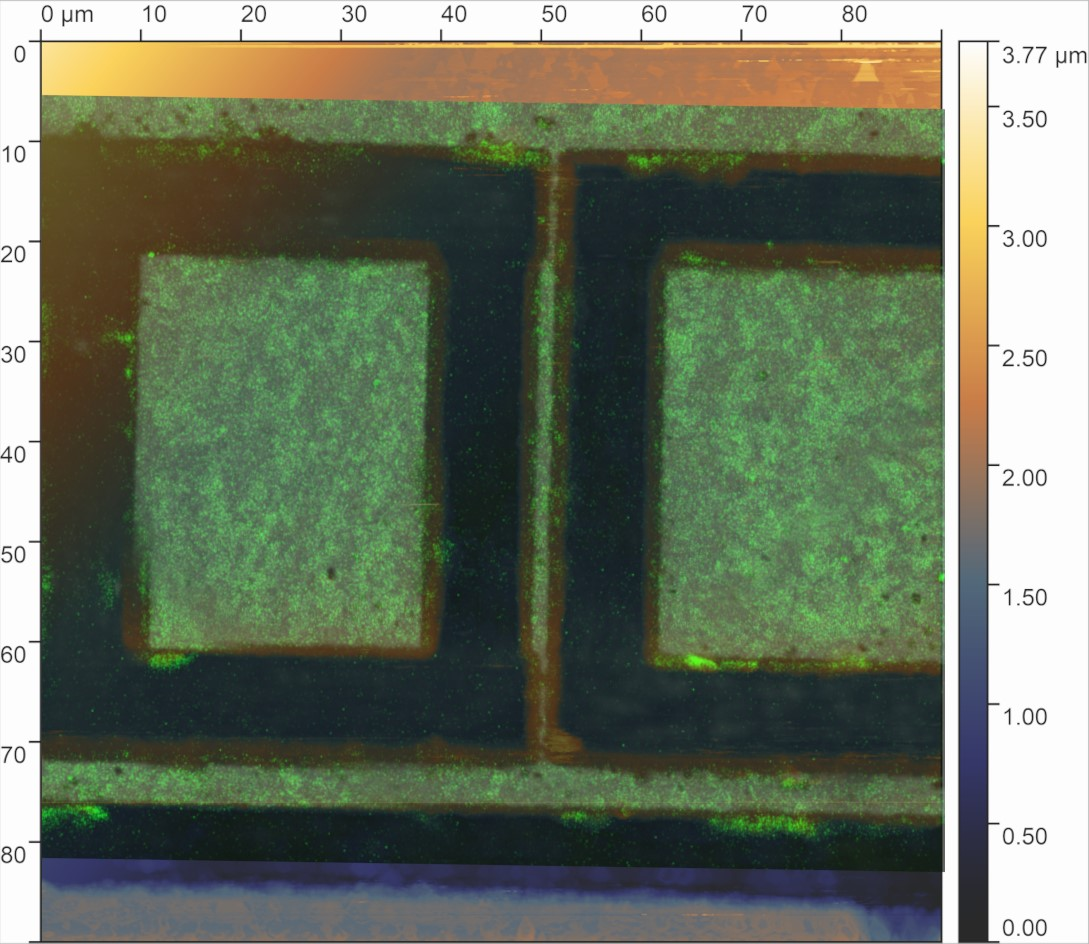
\includegraphics[width=\linewidth]{Chapter7/Figs/Raster/21_comparison.jpg}
    \caption{Contacts 2-1 of the LTLM structure, viewed as a combination of AFM, optical microscopy and fluorescence.}
    \label{fig:21_comparison}
\end{figure}

In figure \ref{fig:21_comparison}, an overlay of the oil-immersion fluorescent microscopy is fitted to the AFM characterisation taken for these two LTLM contacts. The fluorescent microscope imaging has had the transparency adjusted such that the deep blue used for the height associated with the bottom of the trenches is visible enough to observe the topological map. Note that while the visual inspection of these contacts reveals a link between the laser written wires in the lower portion of the channel, the topology reveals a clear lack of ablation in this region. This may have implications for the relative concentration of graphitic material present in the channel, as a lack of ablation will correlate with lower laser power or fluence \cite{Holly1998, kononenko2005}. While the optically transparent diamond has been altered, a speculative conclusion may be that this material is unlikely to be highly graphitic, and hence much more resistive or at least semiconducting in nature. For the AFM topology only please see figure \ref{fig:afm_21_big}.

\subsection{2 Micron Channel IV Characteristics and LTLM Assumptions}
\label{subsubsec:2um channel iv characteristics and ltlm assumptions}
\begin{figure}[H]
    \centering
    \includegraphics[width=\linewidth]{Chapter7/Figs/Raster/21/21 Graphitised linear IV - Data within ±20.0V_IV_plot.png }
    \caption{A linear plot of the averaged IV characteristics across contacts 2-1. Error bars corresponding to a systematic error of 5\% are plotted.}
    \label{fig:21_linear_iv}
\end{figure}

Figure \ref{fig:21_linear_iv} shows the results of several trials of IV measurements across the channel between contacts 2-1. Several qualitative remarks can be made about the relationship displayed here, particularly in contrast to the previous experiments performed by the candidate using metal contacts and a LTLM structure in chapter \ref{ch:electrical_experiments}. Error bars of 5\% are included to account for the spread of data points observed between repeat attempts, and are hence a high estimate of systematic error based on the results themselves.

\begin{figure}[H]
    \centering
    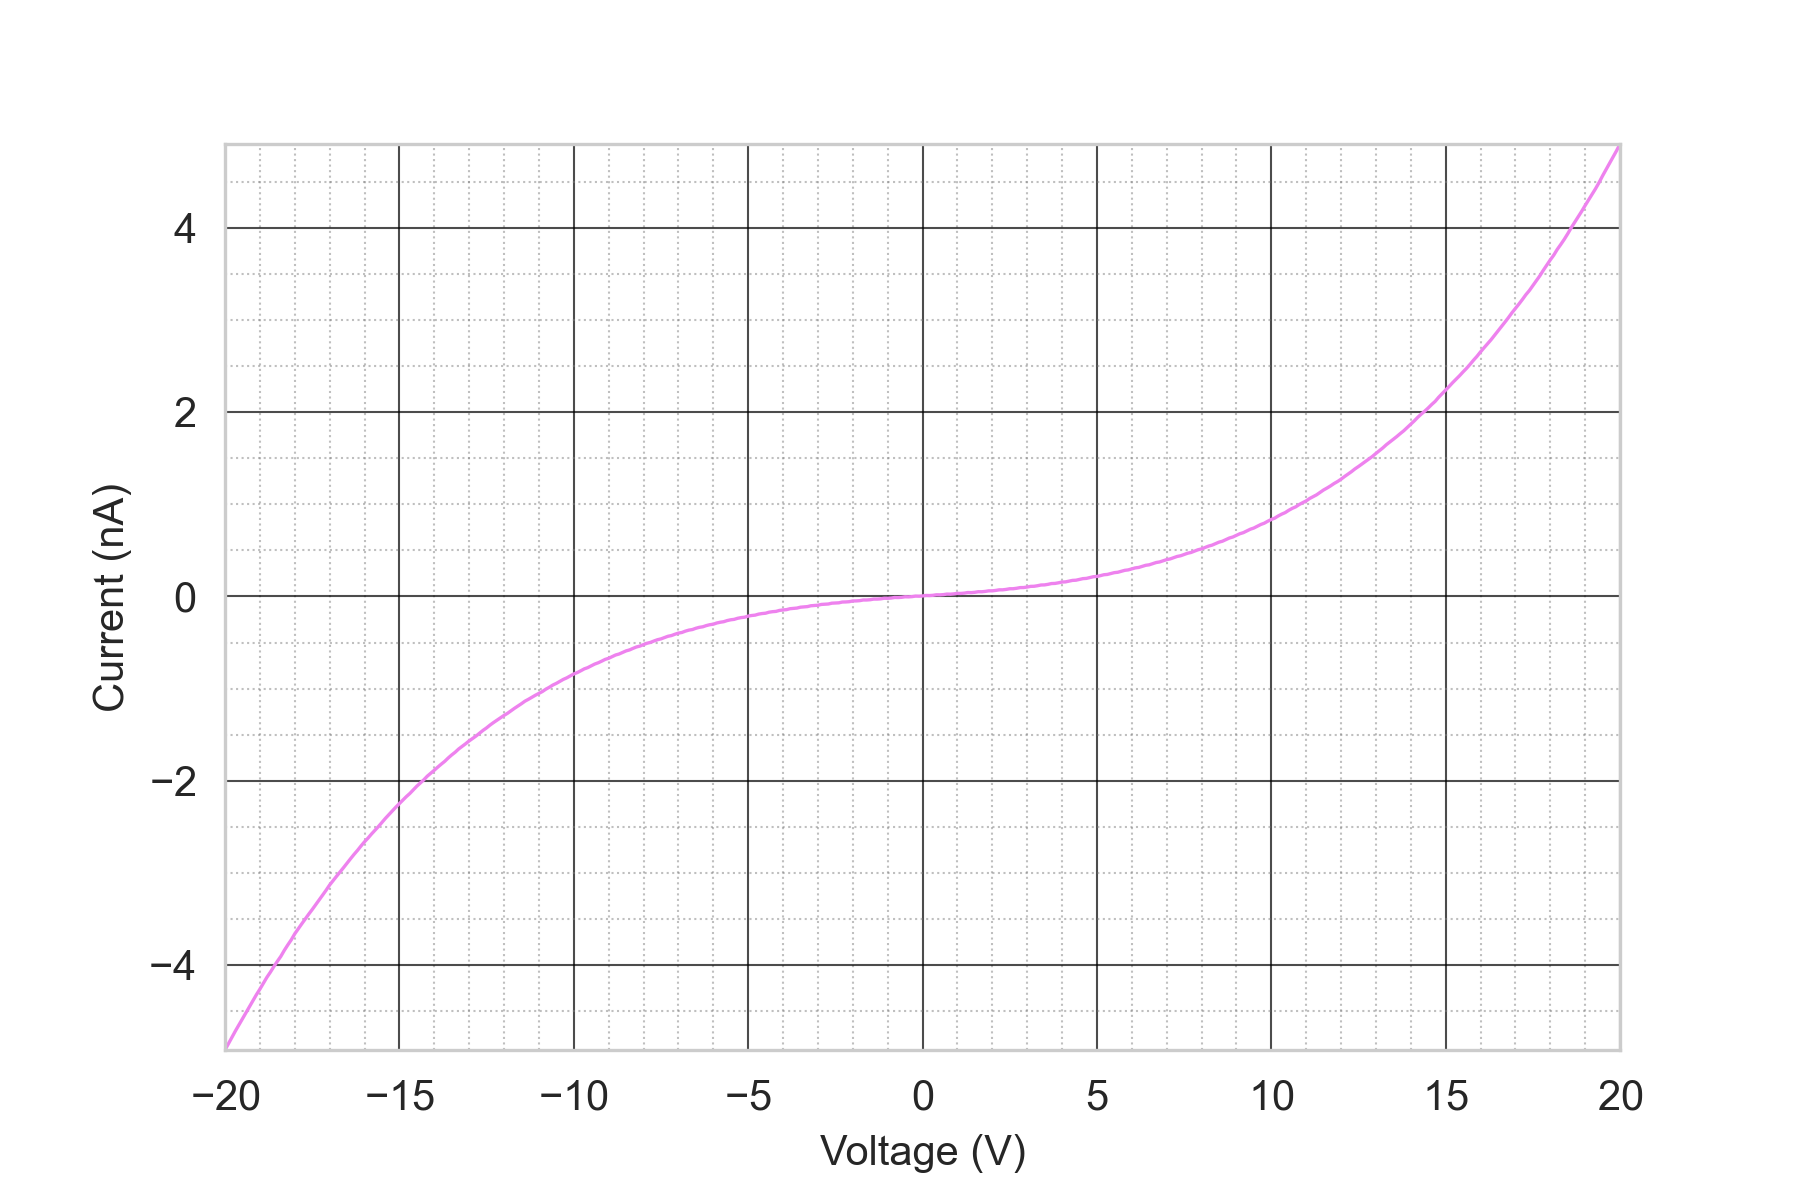
\includegraphics[width=0.8\linewidth]{Chapter7/Figs/Raster/20V IV characteristics at 21 C.png}
    \caption{A linear plot of the measured room temperature IV characteristics across the 2.8~\si{\micro\metre} LTLM channel for sample D (annealed Ti/Pt/Au contacts).}
    \label{fig:d_20v_linear}
\end{figure}

Figure \ref{fig:d_20v_linear} provides a visual reference to sample D, which also used a LTLM device structure for IV characterisation. The phosphorous doped diamond film on sample D was thinner than sample G's, at $\sim$0.3~\si{\micro\metre} against the laser processed $\sim$1.2~\si{\micro\metre} layer. If the only significant factor at play was the thickness of said phosphorous doped layer, with the resistivity remaining the same, then it would be expected that the measured resistance is a factor of 4 lower in the thicker sample. Given that at a bias of 20~\si{\volt}, across a 2.8\si{\micro\metre} channel, sample D had a measured current of $\sim$5~\si{\nano\ampere} and sample G with similar conditions and a $\sim$2~\si{\micro\metre} channel had a measured current of $\sim$93~\si{\milli\ampere}, there is an obvious $10^{7}$ magnitude shift in resistance which must be accounted for. There is also a clear change in behaviour from that of a single Schottky barrier, to what might represent a double Schottky barrier. As noted in the microscopy of channel 2-1, the observed channel width may differ from the designed $2$~\si{\micro\metre}. However, even if the effective channel length is closer to $0.5$~\si{\micro\metre} alongside the known difference in thickness, this presents a geometrical factor of 16 in the observed resistance. Naturally, it is also possible to consider the resistivity as measured via CTLM, which presented a value of $\sim15$~\si{\ohm\centi\metre} with constant current condition of 1~\si{\micro\ampere}. The direct comparative work of Matsumoto et al. \cite{matsumoto2013} gives a value of $\sim9\times10^{-3}$~\si{\ohm\centi\metre} at a constant current condition of 50~\si{\micro\ampere} for similarly doped material. This methodology hence indicated that the majority of the measured resistance was due to the metal contacts, agreeing by and large with the two LTLM samples (C and D). The exact measurements of specific contact resistivity and resistivity do raise questions regarding the quality of metal contacts and homogeneity of highly phosphorous doped diamond, but the key concurring factor with metal contacts on phosphorous doped diamond is that of the extremely high specific contact resistivity that has been observed over a range of annealing conditions. Hence, while the geometry of this laser processed LTLM is largely intended to provide a benchmark for the emitter arrays, a key takeaway from the comparison of IV characteristics represented by figures \ref{fig:21_linear_iv} and \ref{fig:d_20v_linear} may be that the laser written structure is now providing a significantly reduced specific contact resistivity, even prior to the application of LTLM methodology. There are numerous assumptions that must be made to apply the quantitative methodology of the LTLM method in this case, with the channel length, local resistivity, contact wire conductivity and laser written geometry all factors that may affect the results. Be that as it may, the application of LTLM methodology was employed to provide a more direct comparison between metal contacts and laser written contacts.

\subsection{LTLM}
\begin{figure}[H]
    \centering
    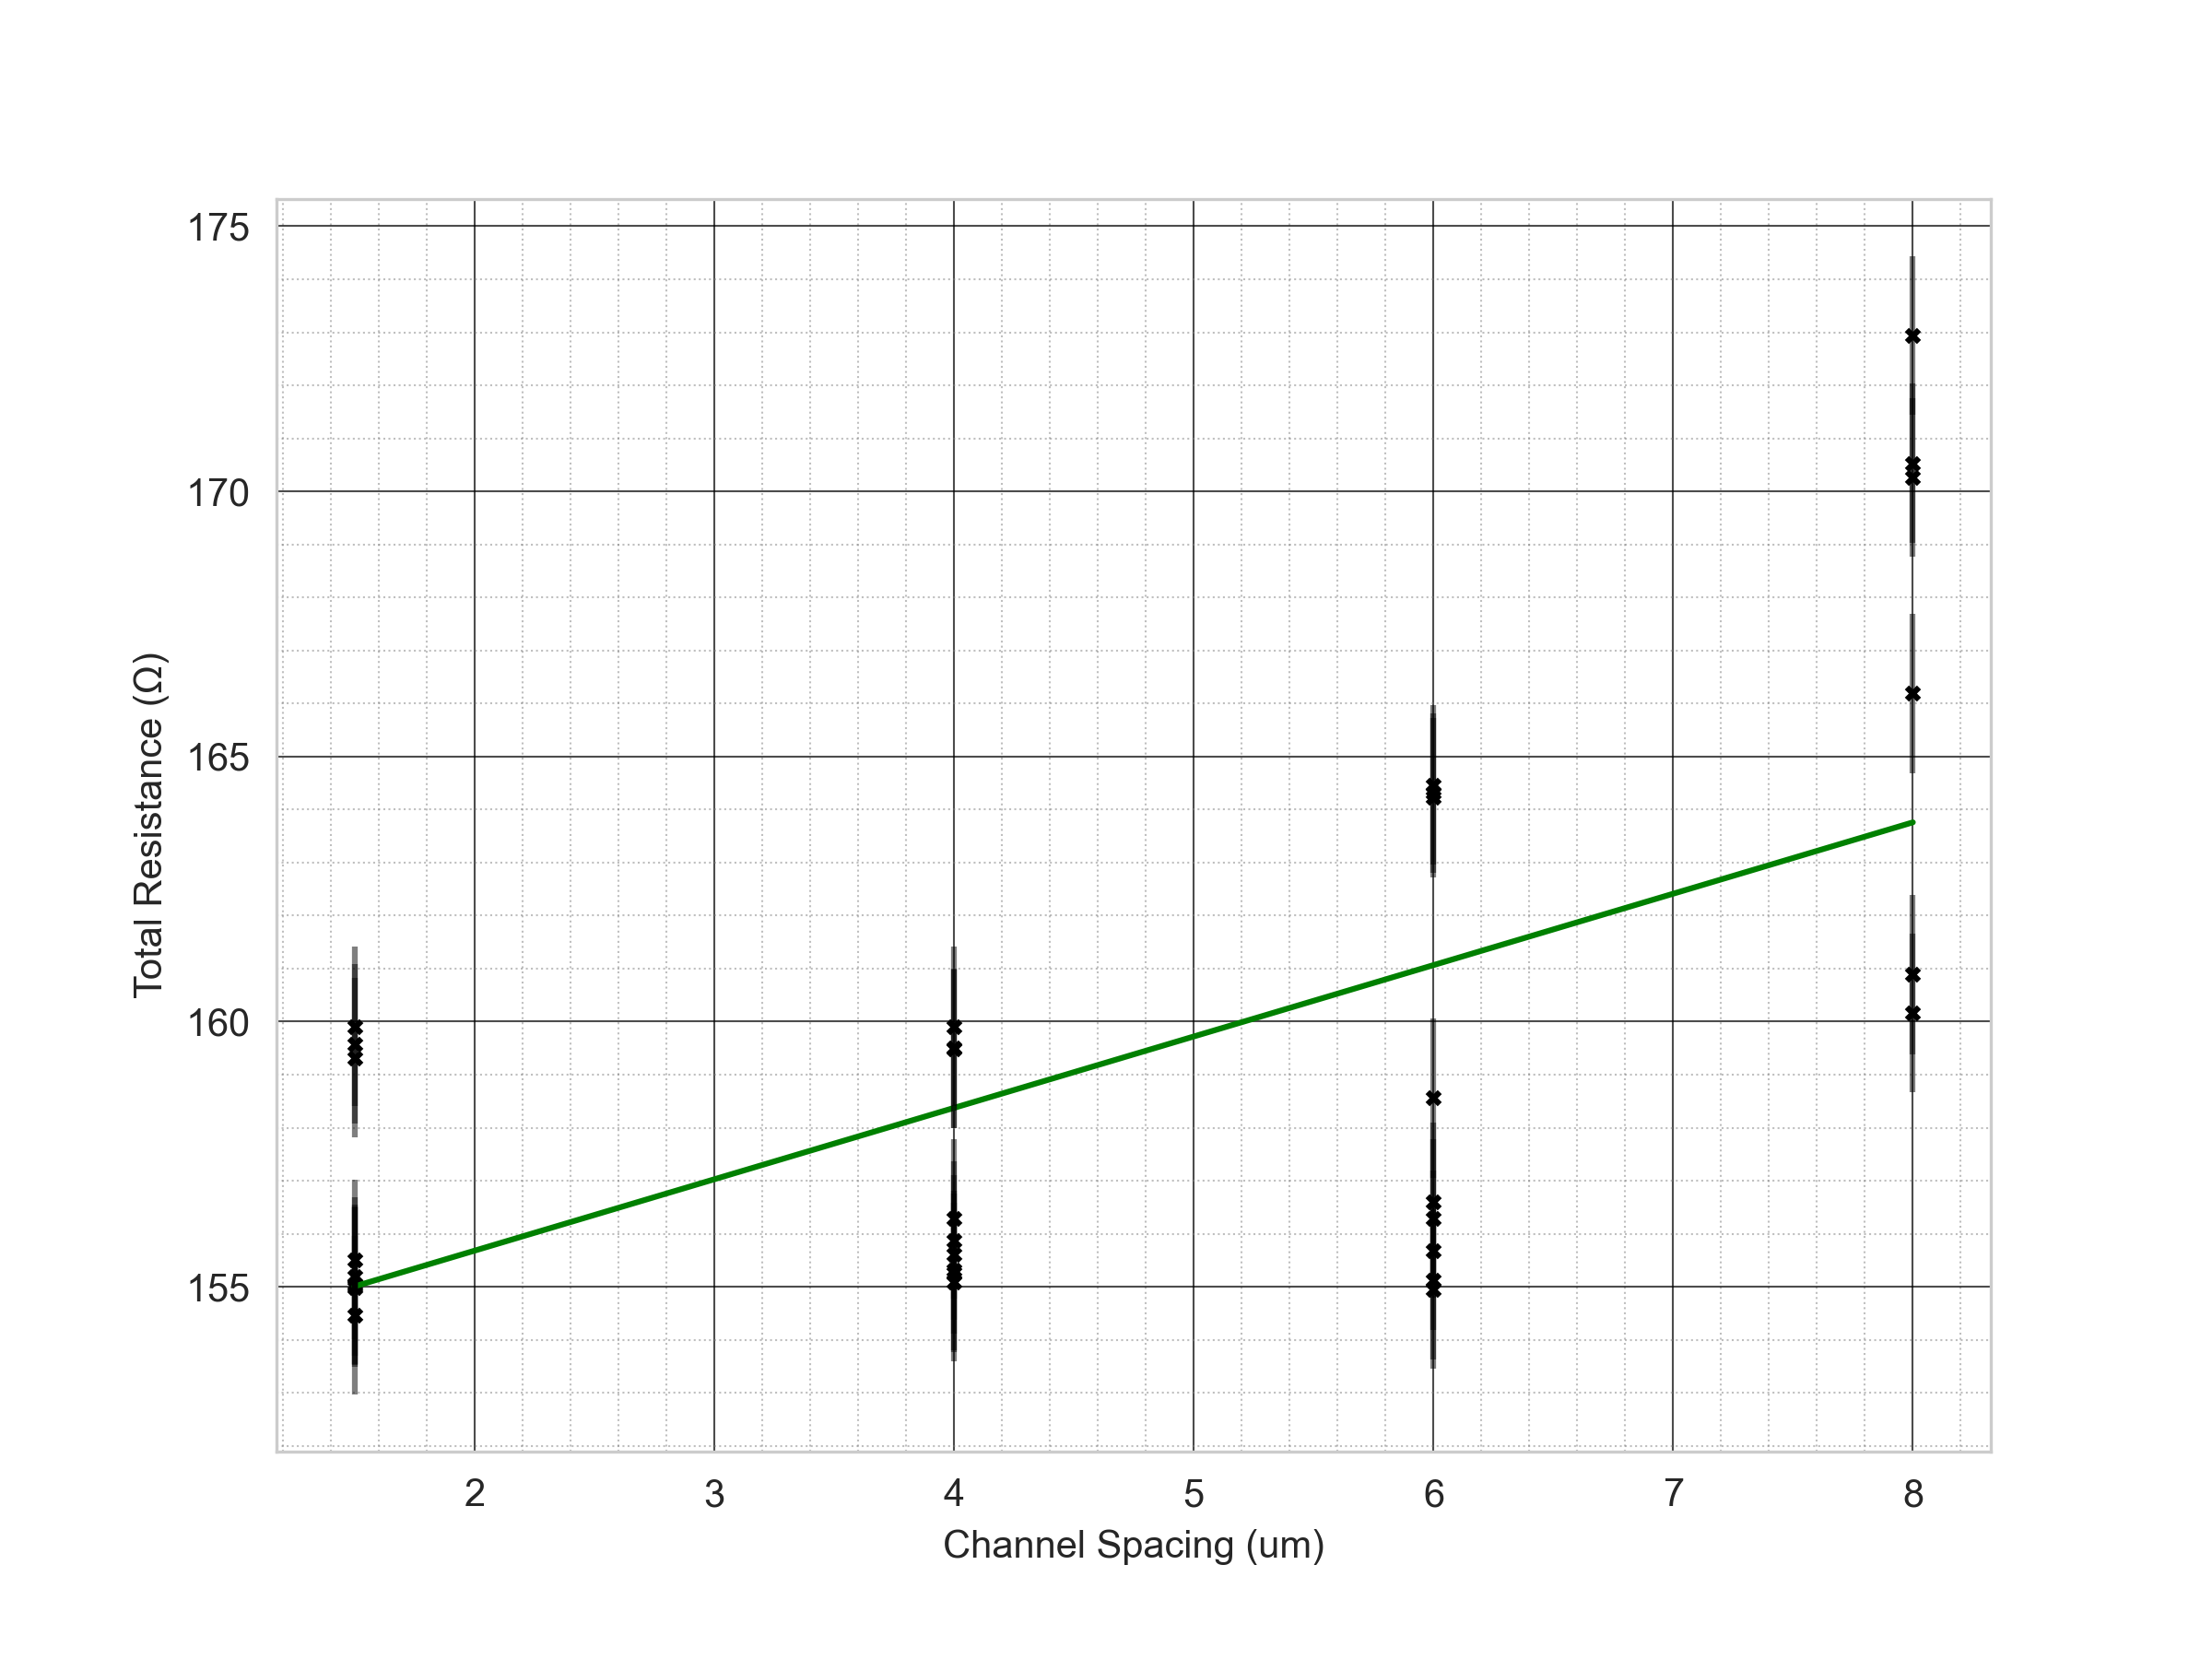
\includegraphics[width=\linewidth]{Chapter7/Figs/Raster/LTLM_graphite_mid(5.0V).png}
    \caption{A linear plot of the total measured resistance against LTLM channel spacing at 5~\si{\volt}, with a line of best fit. Error bars of $\pm$1.5~\si{\ohm} are plotted based on the spread of data observed within each set of IV sweeps, and represent a high estimate of the systematic error.}
    \label{fig:ltlm_graphite_5v_mid}
\end{figure}

Figure \ref{fig:ltlm_graphite_5v_mid} shows the results of several rounds of LTLM experiments. One notable detail is the usage of slightly different channel spacings (1.5, 4, 6, 8 \si{\micro\metre}) when compared to the designed spacings (2, 5, 7, 9 \si{\micro\metre} respectively). This reduction of channel spacing was implemented to better reflect the observed topology of laser written devices, but while the data themselves better match these spacings, this is a difficult measurement to take from the given characterisation techniques and remains as an assumption to allow for plotting. Further to this, the low total resistance observed across all channels is a challenging result to reconcile with the previous wire measurements. This will be explored further in the following sections.

Despite the linear fit seen in figure \ref{fig:ltlm_graphite_5v_mid} having an R$^{2}$ value of 0.39, the extracted specific contact resistivity is $5.5\times10^{-5}$~\si{\ohm\centi\metre\squared}, representing the lowest specific contact resistivity to highly phosphorous doped diamond of any devices presented in the literature. It is important to note the voltage at which this set of data are obtained, 5~\si{\volt}. This is a reasonable estimate of the linear, forward bias region of one of the two Schottky barriers, but the linear IV characteristics for all channel spacings reflect the lack of comparison to that of ohmic contacts around the 0~\si{\volt} region. 

\subsection{Line of Best Fit and LTLM Parameters}
\begin{figure}[H]
    \centering
    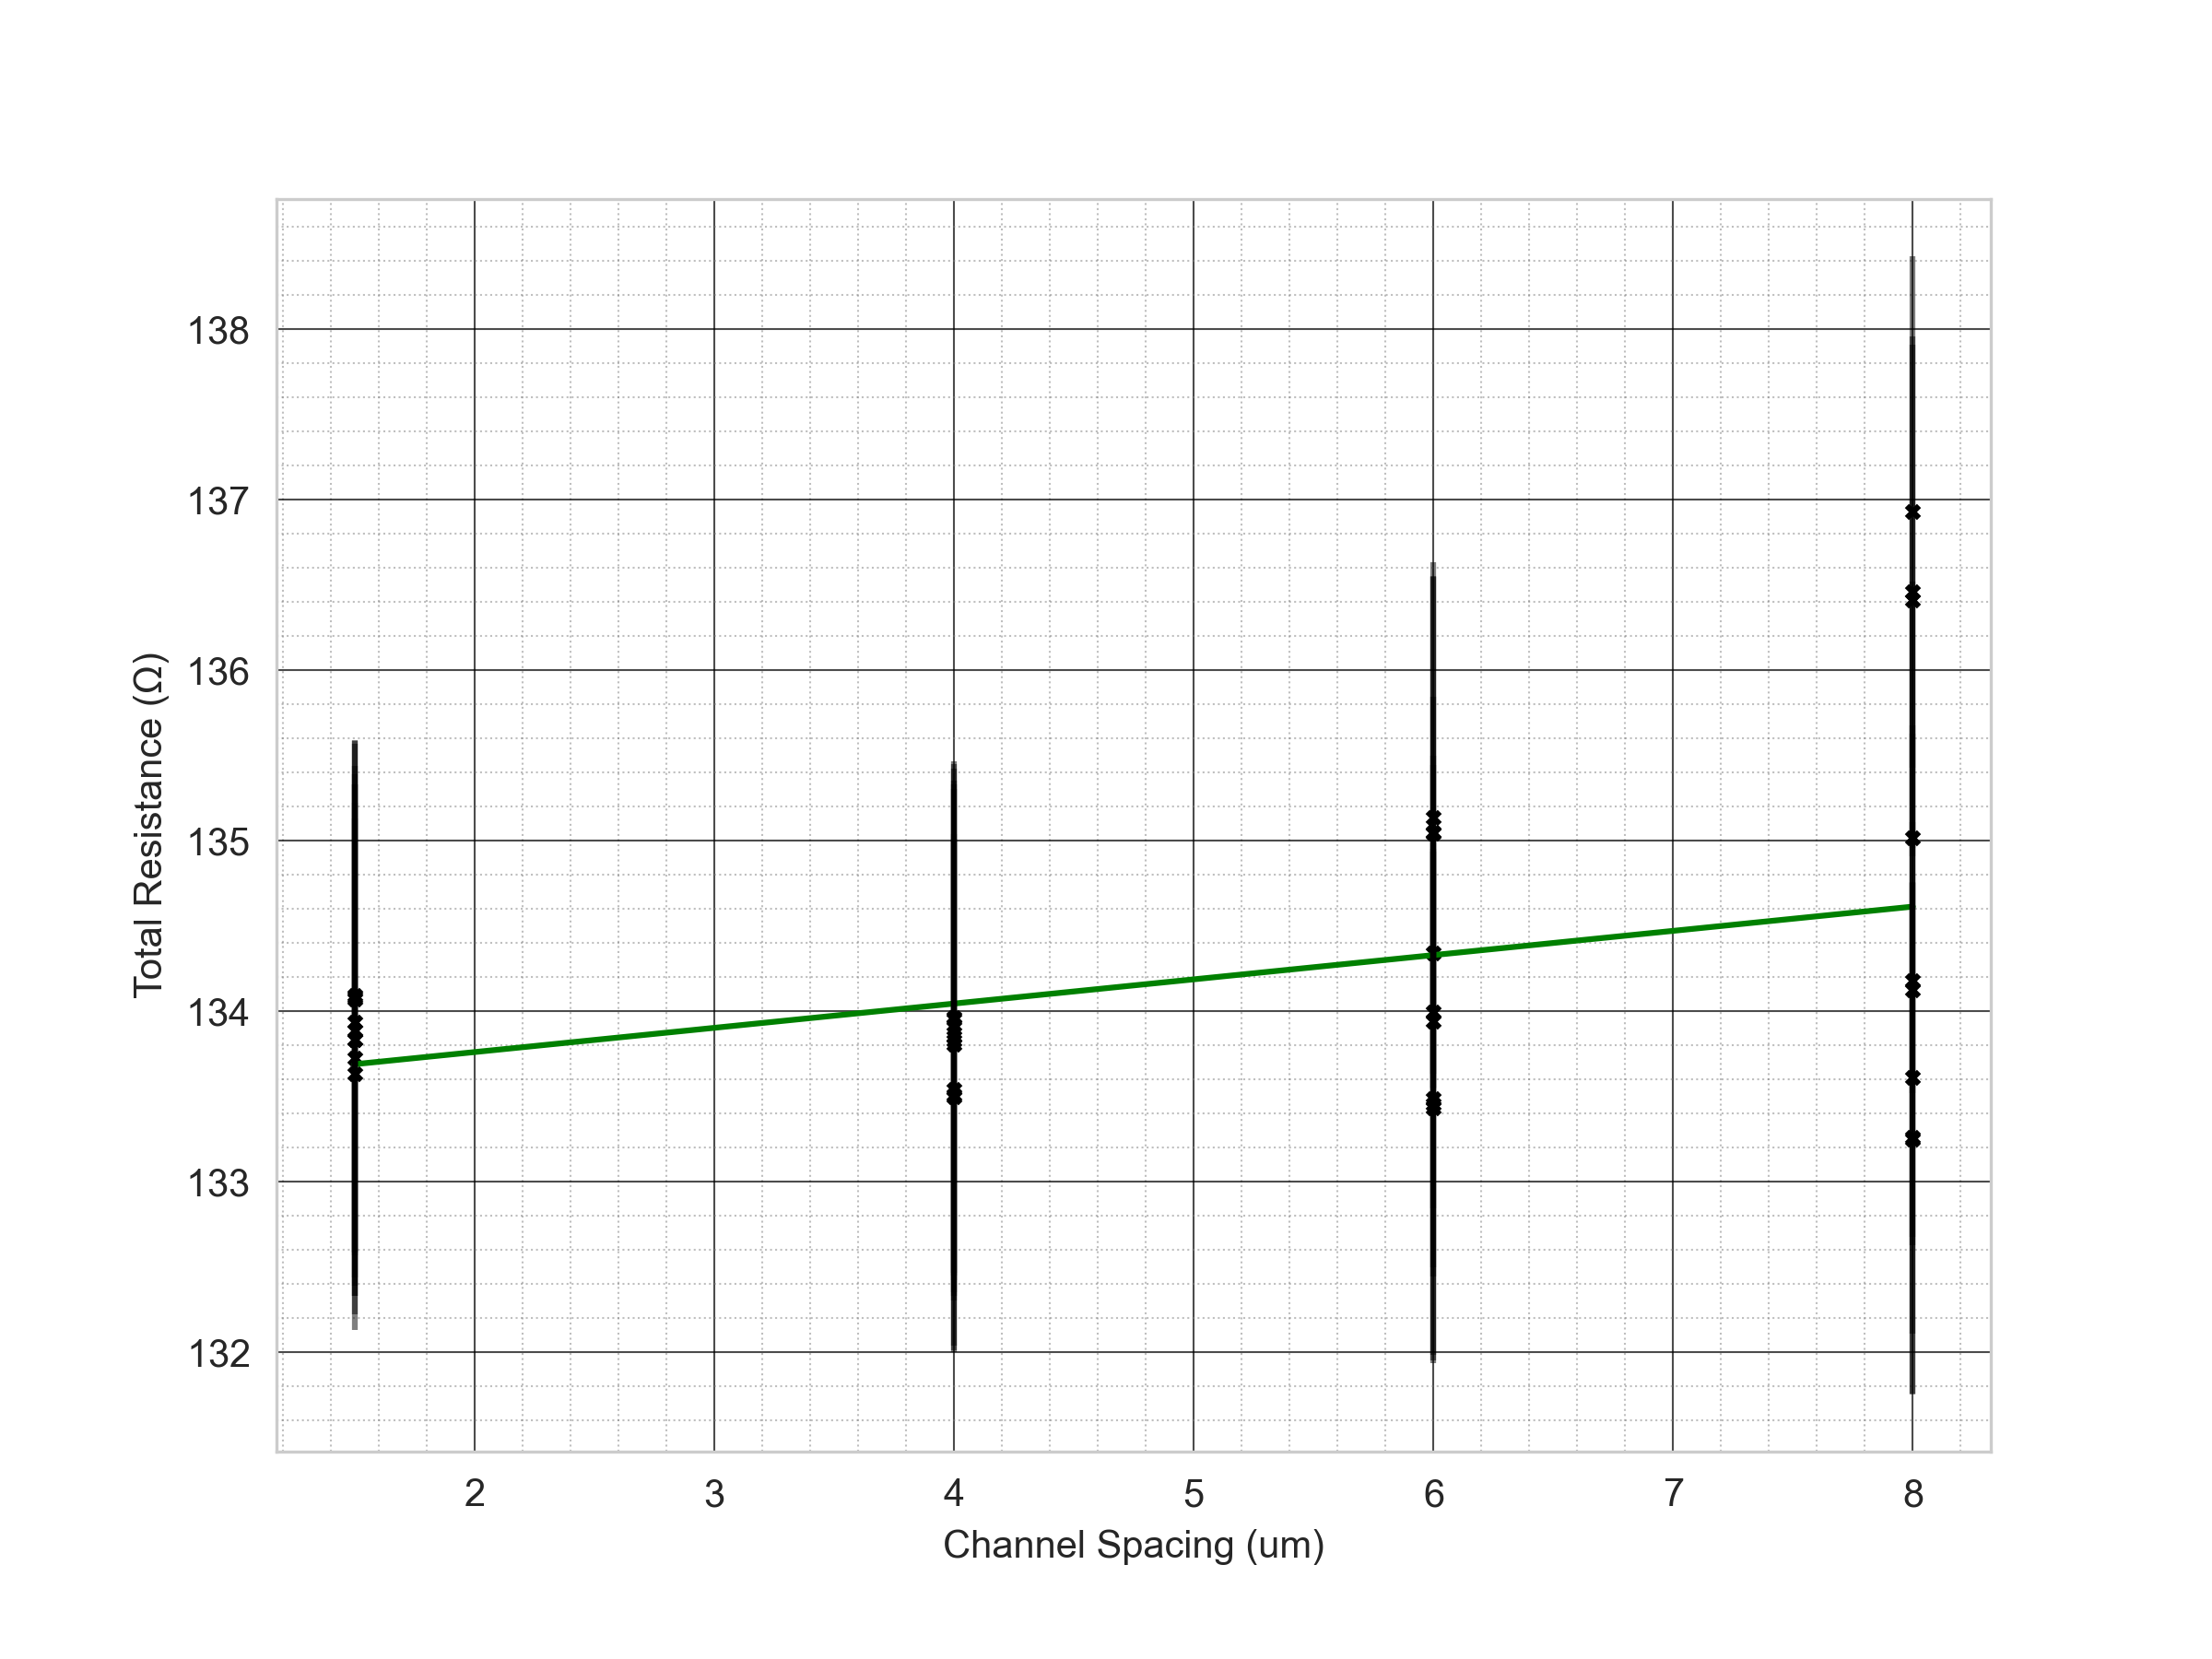
\includegraphics[width=\linewidth]{Chapter7/Figs/Raster/LTLM_graphite_mid(10.0V).png}
    \caption{A linear plot of the total measured resistance against LTLM channel spacing at 10~\si{\volt}, with a line of best fit. Error bars of $\pm$1.5~\si{\ohm} are plotted based on the spread of data observed within each set of IV sweeps, and represent a high estimate of the systematic error.}
    \label{fig:ltlm_graphite_10v_mid}
\end{figure}

Figure \ref{fig:ltlm_graphite_10v_mid} shows the LTLM plot for resistance data collected at a potential bias of 10~\si{\volt}. The line of best fit in this case is very poor, with an R$^{2}$ value of 0.15. The measured resistance has been lowered relative to the 5~\si{\volt} measurements for all channel lengths, which may be due to the voltage-dependent conductivity of laser processed wires.

As seen, when the LTLM methodology is applied to differing voltages, the resulting line of best fit can change quite dramatically in quality relative to the data. However, while the specific values of the total measured resistance do generally reduce at higher voltages, the rough trendlines observed in figures \ref{fig:ltlm_graphite_5v_mid} and \ref{fig:ltlm_graphite_10v_mid} are still present. It is also worth noting that any line which passes through the LTLM data presented here will have similar orders of magnitude for the specific contact resistivity and sheet resistance/resistivity, regardless of the resulting R$^{2}$ value. 

This allows for some speculative comparison to be made to work such as Valappil et al. \cite{valappil2022, valappil2023}, who demonstrated nanocarbon specific contact resistivitys of $1\times10^{-3}$~\si{\ohm\centi\metre\squared} for the voltage range of 5--10~\si{\volt}. Matsumoto et al \cite{matsumoto2013} demonstrated thermally graphitised CTLM specific contact resistivitys of $0.9$~\si{\ohm\centi\metre\squared}, notably at around the 2~\si{\volt} mark. Finally, previous literature values such as that of Kato et al \cite{kato2009} at $2\times10^{-3}$~\si{\ohm\centi\metre\squared} may also be considered, though this publication did not use the constant current condition necessary for CTLM methodology.

The error present with any linear fit in figure \ref{fig:ltlm_graphite_5v_mid} prevents any conclusive comparison to be made with these examples, as a linear fit to these data is speculative at best. A useful consideration may be the range of linear fits that are possible given this dataset, as the specific contact resistivity estimation of $1\times10^{-5}$~\si{\ohm\centi\metre\squared} is two orders of magnitude lower to comparable contacts made using nanocarbon or thermally graphitised contacts on highly phosphorous doped material.

Another consideration is the possibility of the electrical contacts deteriorating over time, or with consecutive electrical measurements. The data used for figure \ref{fig:ltlm_graphite_5v_mid} spans multiple days, with repeat measurements on those days. While a good degree of repeatability was observed throughout the experimental process, the similarity between total measured resistances across the range of channels does raise questions concerning the source of any error. Although data that were likely affected by poor contact placement have already been discarded, the factor of variable conductivity within the wires themselves, and the potential impact of this upon the graphite/diamond/graphitic structure formed, is more difficult to quantify. Finally, the discrepancy between the measured resistance across LTLM contacts and the wire test structures must be considered. 

\subsection{Missing Resistance}
\label{subsubsec:missing_resistance}
As previously stated in section \ref{subsubsec:2um channel iv characteristics and ltlm assumptions}, the IV characteristics of the LTLM structure were performed with an observation of repeatability between differing days and across all four channel spacings. However, testing of emitter structures revealed a significantly lower base current, of the order of \si{\micro\ampere}. This is in line with the previous electrical measurements across wire testing structures in section \ref{subsec:testing_of_surface_graphitic_wires}, and hence the LTLM measurements require further exploration.
\clearpage

\begin{figure}[H]
    \centering
    \includegraphics[width=\linewidth]{Chapter7/Figs/Raster/All Graphitised linear IV - Data within ±20.0V_IV_plot.png}
    \caption{A linear plot of the averaged IV characteristics across all channel spacings with percentage error bars of 5\%.}
    \label{fig:all_linear_iv}
\end{figure}

\begin{wrapfigure}{r}{0.4\linewidth}
  \centering
  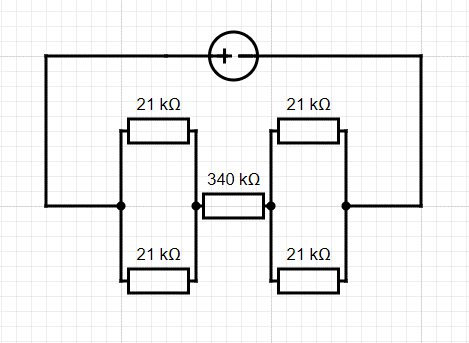
\includegraphics[width=\linewidth]{Chapter7/Figs/Raster/missing_resistance_circuit.png}
  \caption{A circuit diagram of the expected LTLM structure for a 4~\si{\micro\metre} channel.}
  \label{fig:missing_resistance}
\end{wrapfigure}

Figure \ref{fig:all_linear_iv} shows the full range of IV characteristics for the LTLM structure. Each channel was swept at least 12 times, ranging from $\pm1$~\si{\volt}, to $\pm20$~\si{\volt}, with the average data presented in the figure. A simplified circuit diagram of the structure, as it was tested, may resemble a series of parallel resistors, along with the channel resistor. Taking an average value of resistivity for the 10~\si{\micro\metre} wires of $0.14$~\si{\ohm\centi\metre}, and estimating the distance via the two conductive paths from the probe to the LTLM channel as 162~\si{\micro\metre}, thickness 0.5~\si{\micro\metre}, the predicted pair of resistors for each contact wire are 21~\si{\kilo\ohm}. Given a channel spacing of 4~\si{\micro\metre}, with resistivity of phosphorous doped diamond as quantified by CTLM at 15~\si{\ohm\centi\metre}, thickness 1.2~\si{\micro\metre} and contact width 60~\si{\micro\metre}, it can be expected for the channel resistance to be approximately 340~\si{\kilo\ohm}. This is represented by figure \ref{fig:missing_resistance}.

This resistance is not reflected in the LTLM data, despite further experiments on emitter structures following this expectation well. As this is the case for all LTLM data collected in this set of experiments, which involved at minimum two days of data collection, it is unclear why this is the case. The data point towards an unintended conduction channel being responsible for the observed IV characteristics, despite control experiments ensuring that no conductive channel was present without the probes actively in contact with the LTLM test structure, as is standard practice. Furthermore, the same probes and experimental setup were used to provide testing data on wire structures, with no issues identified with any of those electrical sweeps or the data in follow-up analysis. Despite these checks, the LTLM data presented here must be considered to be affected by a systematic error, due to the large discrepancy in observed resistance and the resistance of all other test structures.

Finally, with the benefit of additional data through emitter testing and another LTLM experiment that will be presented in the following sections, a more realistic peak current value may be expected at the 3~\si{\micro\ampere} level for channel spacings comparable to that of the LTLM structure. While this is certainly not a full TLM methodology, if the current observed in all of the LTLM measurements presented here were affected by a factor of $10^{5}$ shift due to an unknown systematic error, then the actual specific contact resistivity would be approximately 1~\si{\ohm\centi\metre\squared}. This is the same order of magnitude that was observed via thermal graphitisation \cite{matsumoto2013}, and would place laser processing firmly among the established methods of reducing specific contact resistivity to highly phosphorous doped diamond, even given the lower resistivity previously measured on these samples using CTLM which will make any ohmic contacts harder to form. 

\section{Second Round Of LTLM}
\label{subsec:ltlm2_lost_data}
As it was established in section \ref{subsubsec:missing_resistance} that the collected LTLM data had an inexplicable systematic error following measurements of emitter structures, a fresh set of measurements were taken with new micro-probes and another solvent clean. To ensure that these data would have a higher reliability, the additional step of taking measurements under illumination and in complete darkness was undertaken. The intention of this, along with a more thorough experimental process overall was to ensure that the IV data was both repeatable and also sensible in the context of phosphorous doped diamond samples.

\subsubsection{IV Characteristics (Light/Dark)}

\begin{figure}[H]
    \centering
    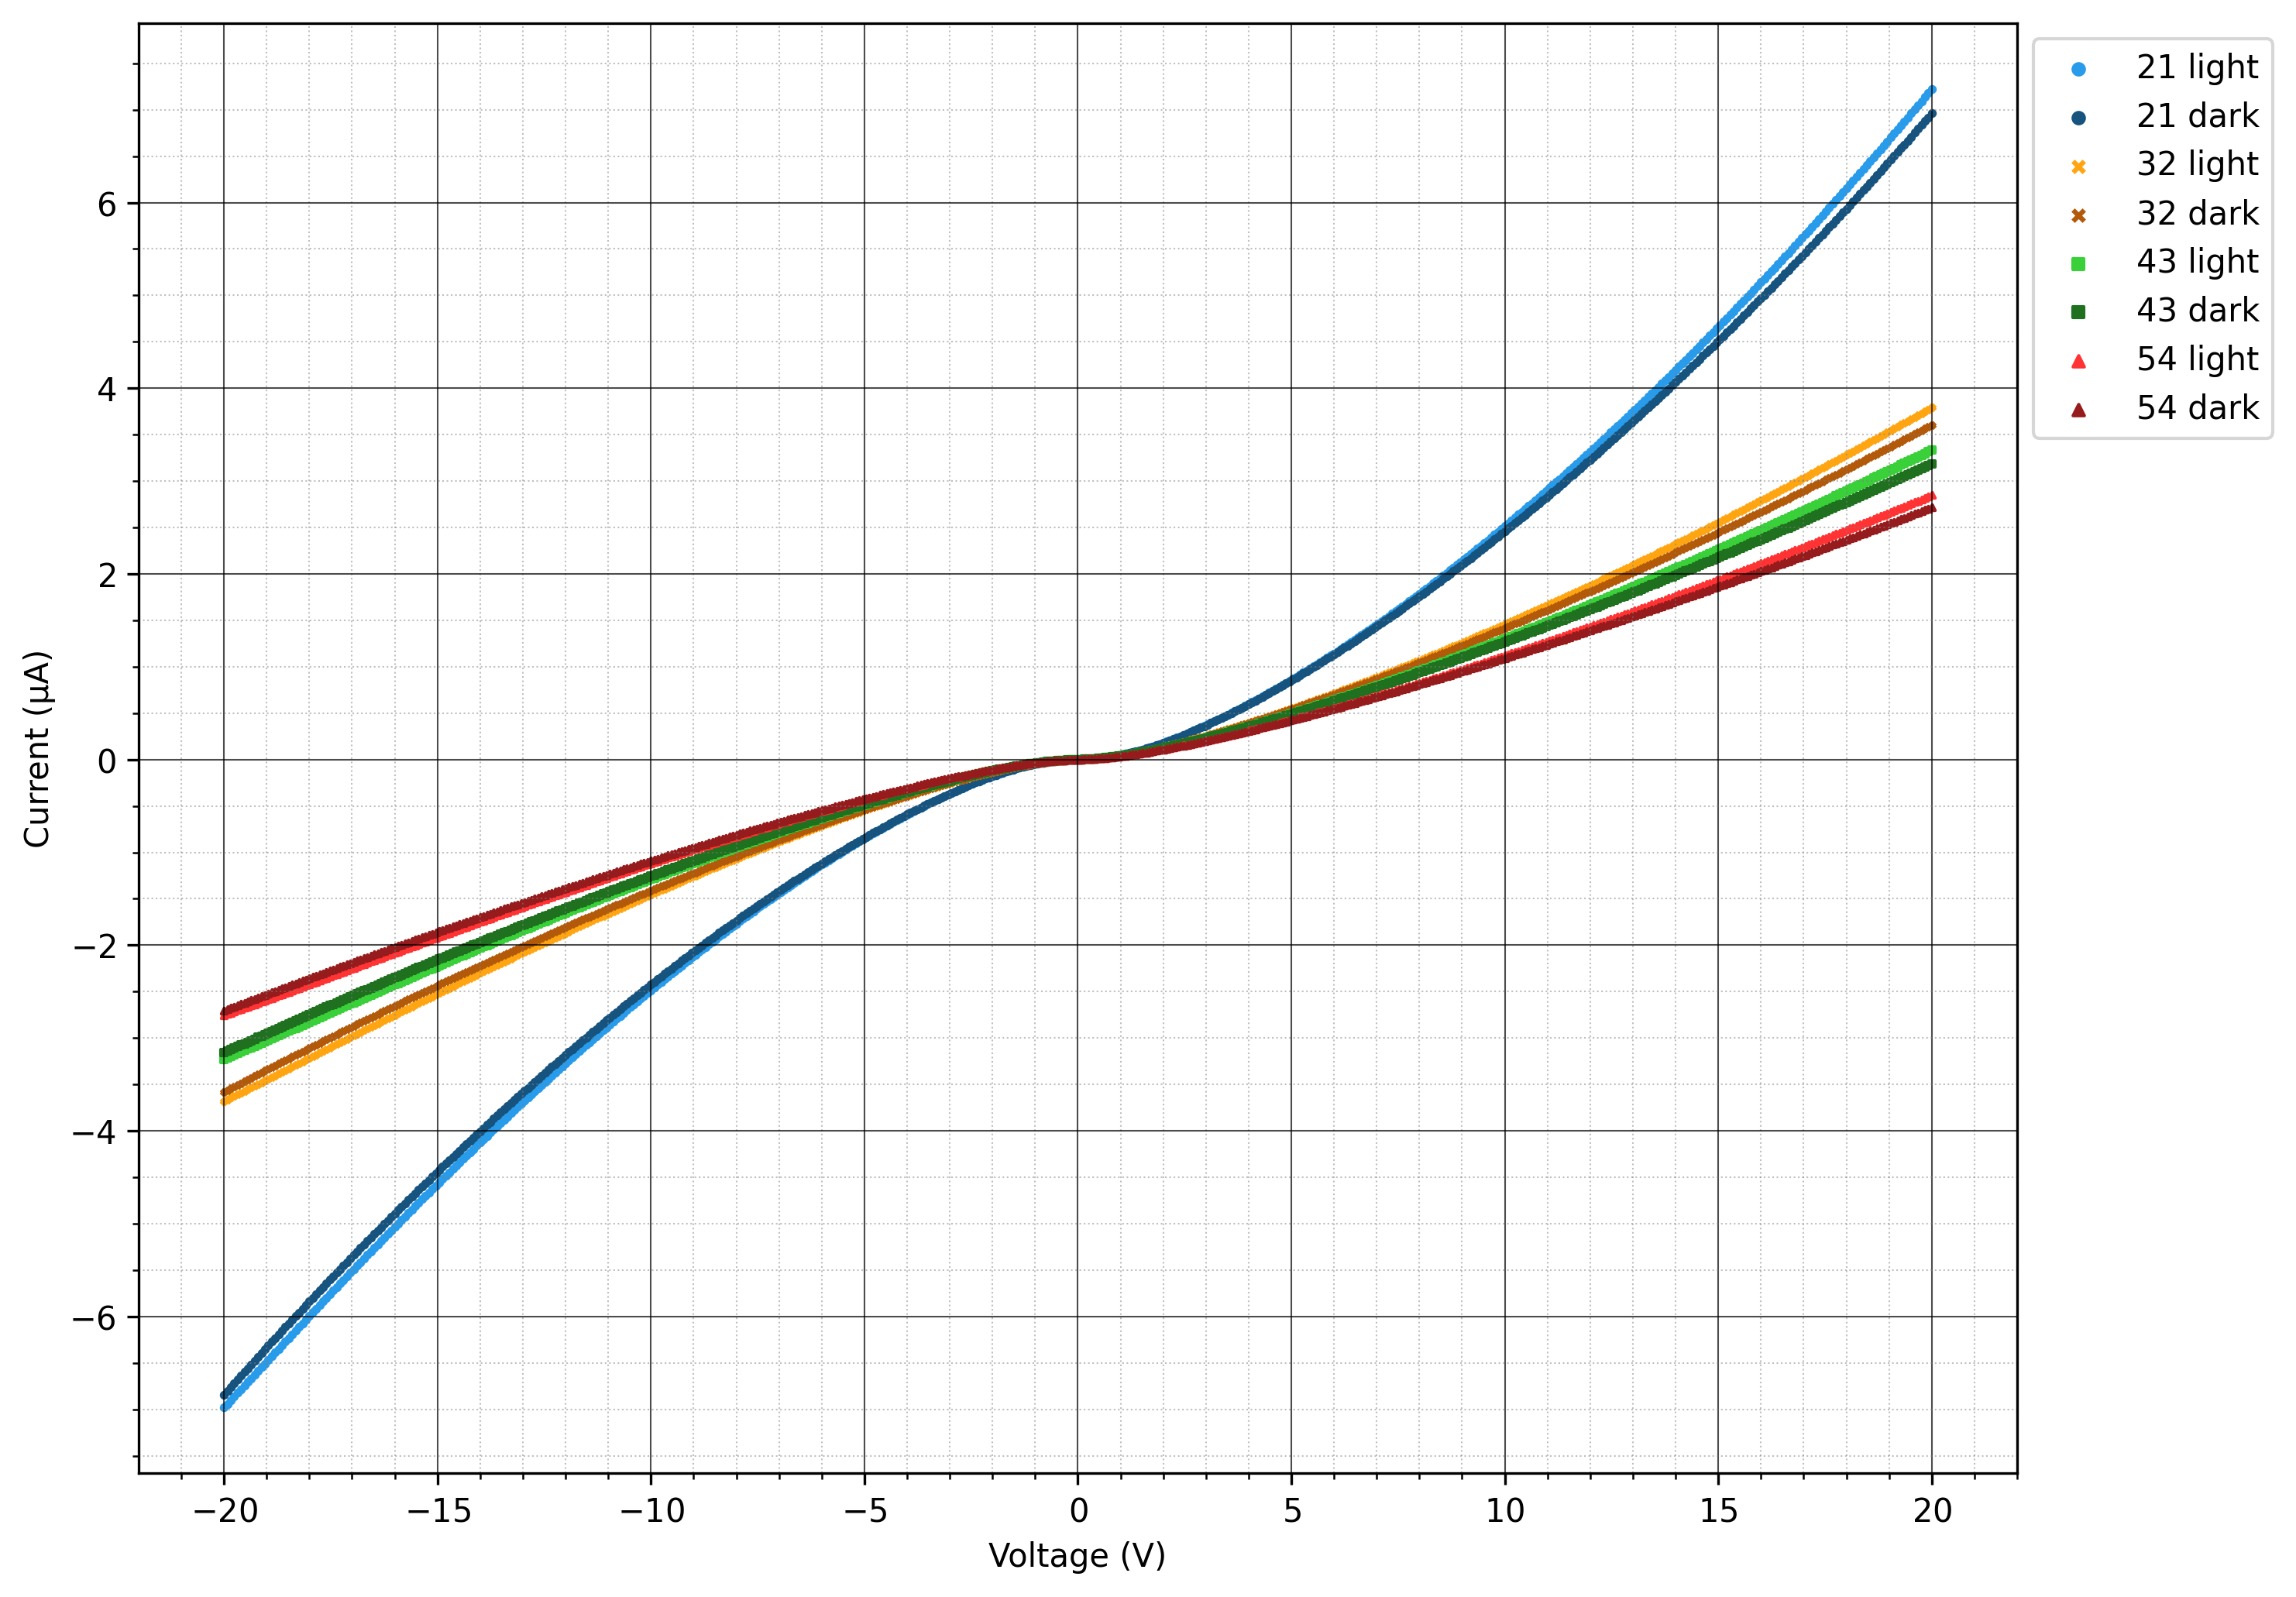
\includegraphics[width=\linewidth]{Chapter7/Figs/Raster/Lost Data/20V Combined IV Characteristics for All Conditions.png}
    \caption{A linear plot of the averaged IV characteristics across all channel spacings, $\pm20$~\si{\volt}, under bright illumination or in darkness.}
    \label{fig:lost_iv_20v}
\end{figure}

Figure \ref{fig:lost_iv_20v} shows the full set of IV characteristics taken during this second run of LTLM measurements. Each set of scatter points represents 3 datasets, averaged together with 501 data points. The same probe positions as for the previous LTLM measurements were used. Lighter and darker colours are used to help provide a visual difference between the light and dark datasets respectively, which diverge in a consistent manner. The reduction of measured total resistance under illumination provides a clear indication of semiconducting properties, with the conductive path expected to be within the phosphorous doped diamond surface layer. The observed current matches the conclusions drawn from the previous LTLM testing, with the correct order of magnitude as expected for contacts of $\sim1$~\si{\ohm\centi\metre\squared} beyond the low voltage region. Note that in contrast to the previous LTLM IV plots which had 5\% error bars to account for the spread of datapoints observed during testing, the data in this figure were observed to be highly repeatable and the error can instead be presumed to be close to the limit imposed by that of the B1500 probe station. As calibrated, this is below $1$~\si{\nano\ampere}, approaching $1$~\si{\pico\ampere}, and is hence not visible in the plots of currents as error bars.

\begin{figure}[H]
    \centering
    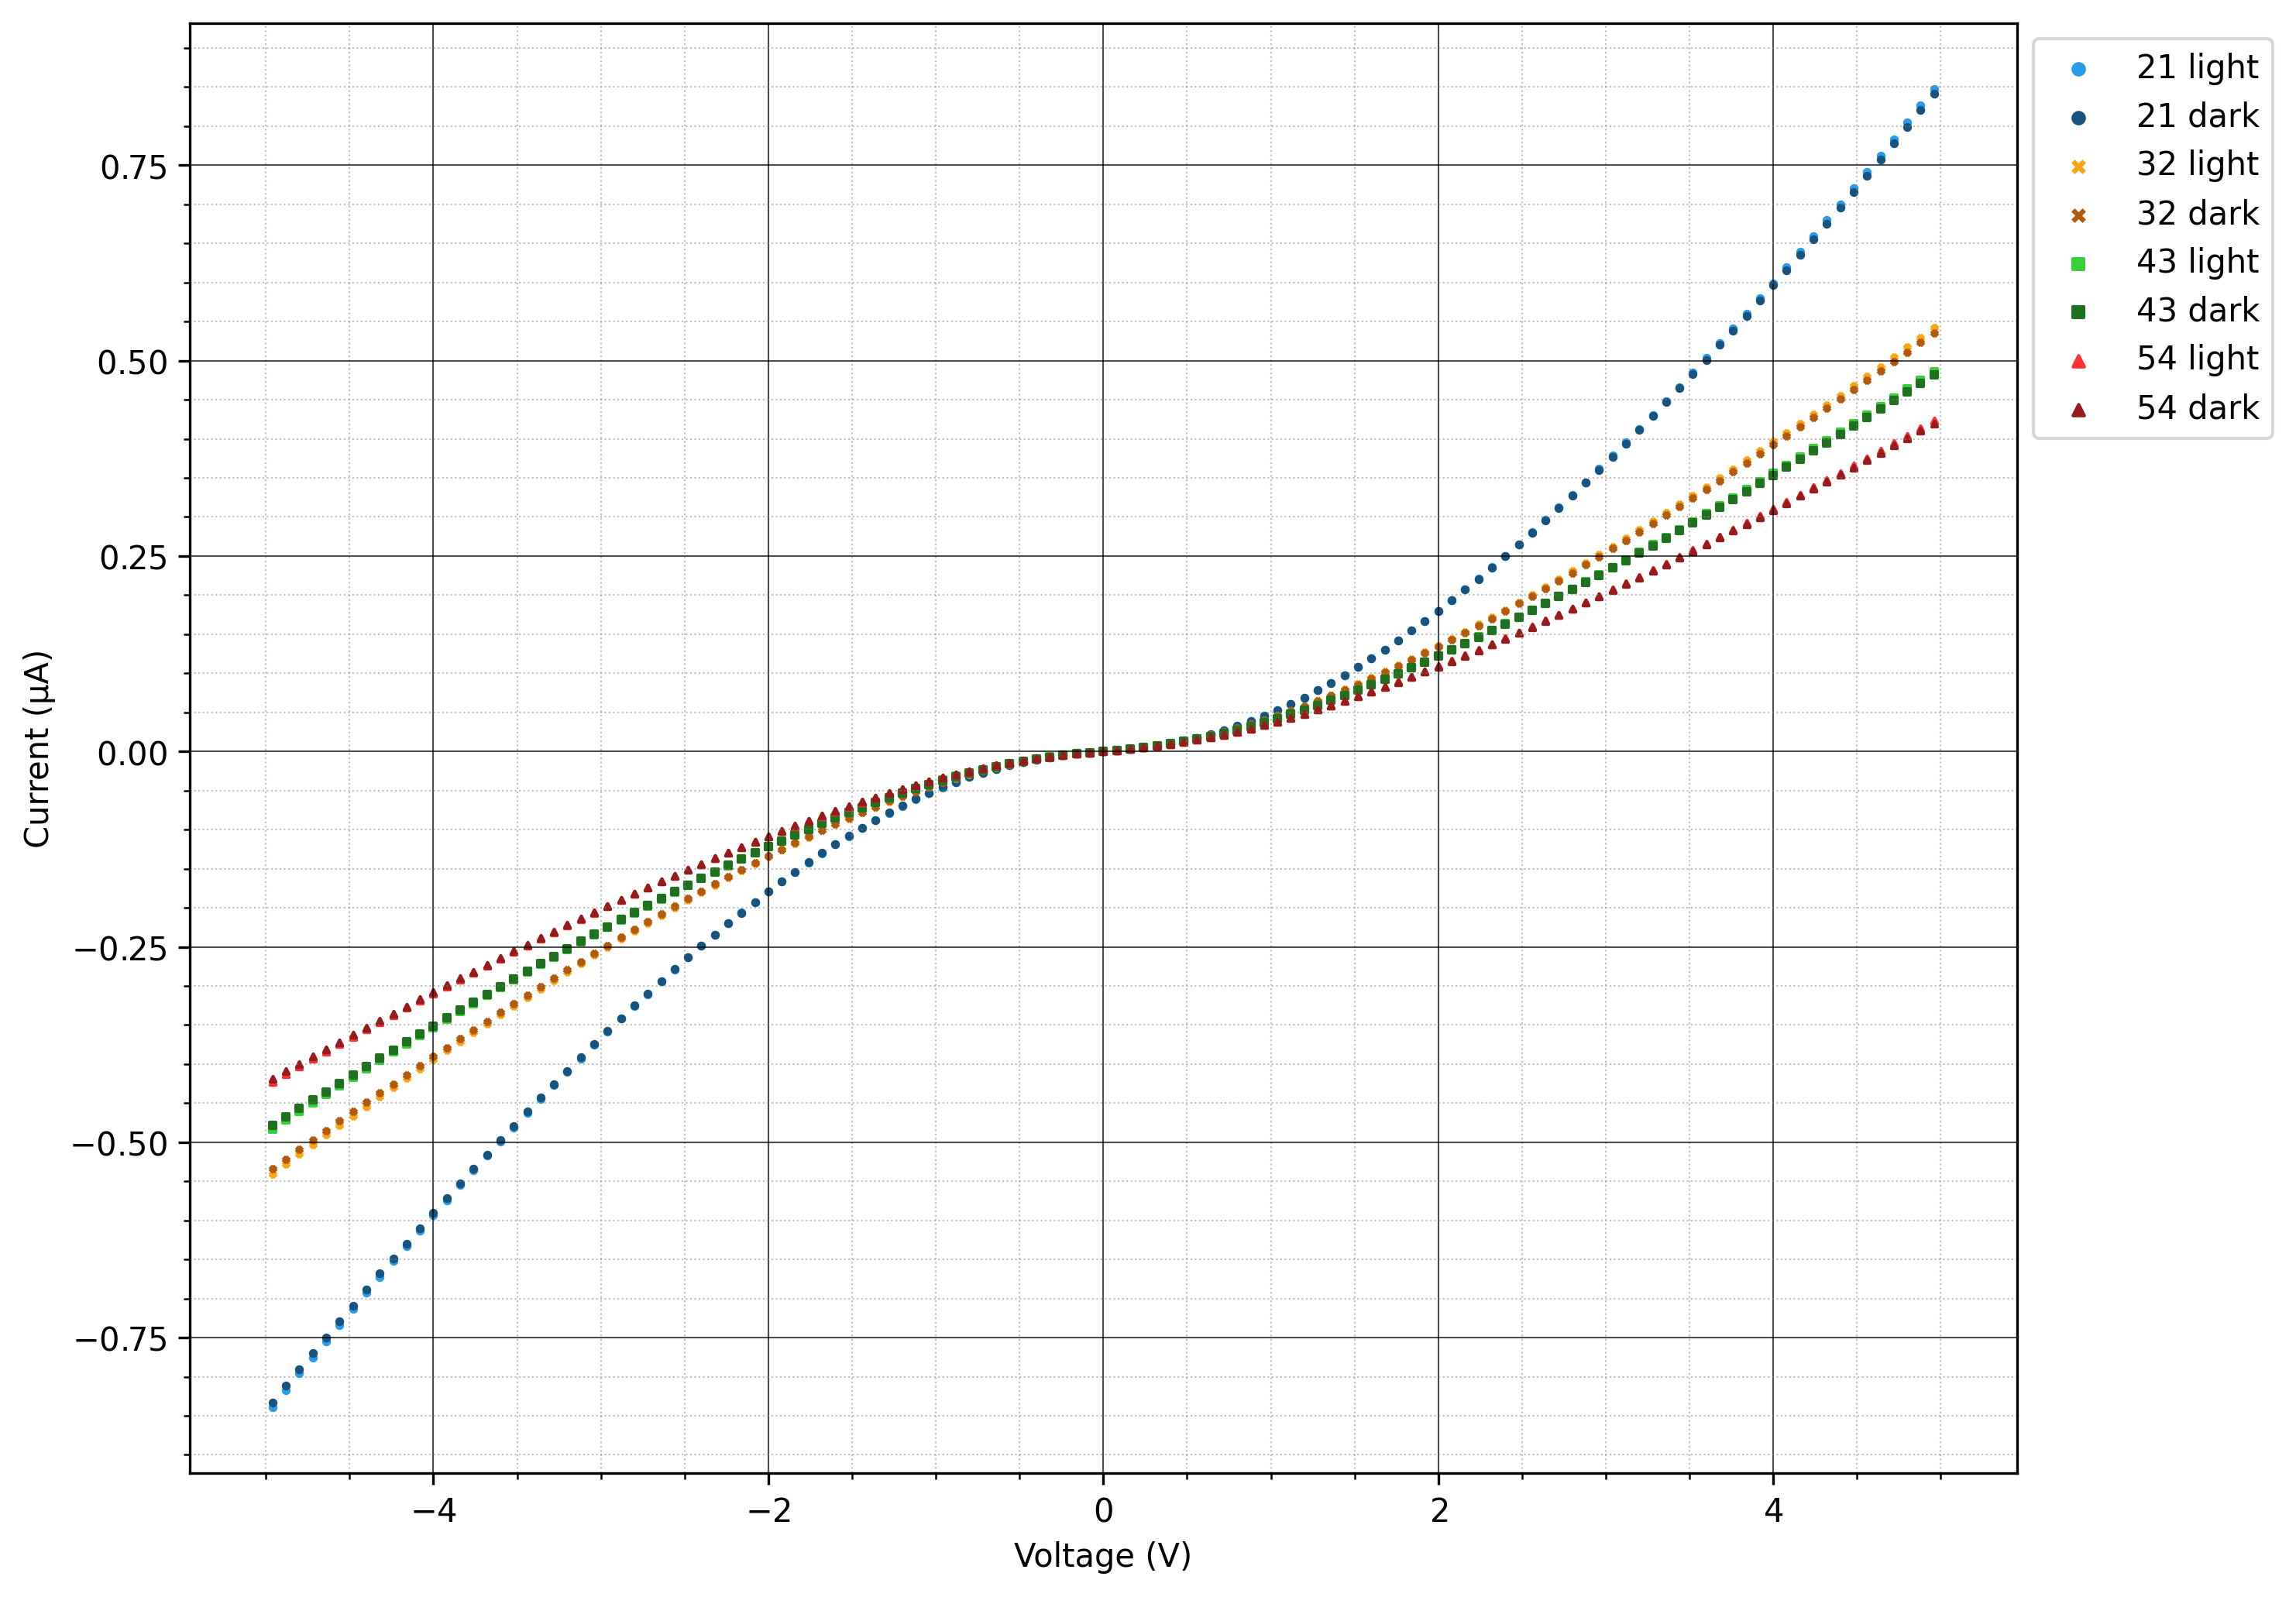
\includegraphics[width=\linewidth]{Chapter7/Figs/Raster/Lost Data/5V Combined IV Characteristics for All Conditions.png}
    \caption{A linear plot of the averaged IV characteristics across all channel spacings, $\pm5$~\si{\volt}, under bright illumination or in darkness.}
    \label{fig:lost_iv_5v}
\end{figure}

In figure \ref{fig:lost_iv_5v}, the low voltage region in particular is plotted. At this scale, it is difficult to see the marginal reduction in resistance due to illumination relative to the dark characteristics. It is also considered that the 501 datapoints used for these sweeps are adequate to resolve the low voltage region, which may be defined as $\pm1$~\si{\volt}. Further sampling would provide more certainty for comparisons between channels, but the potential for error due to micro-probe positioning negates the slight gains in precision that could be obtained with higher datapoints. Within this bias region, neither of the double Schottky barriers are sufficiently biased to overcome the Schottky barrier heights. As for figure \ref{fig:lost_iv_20v}, the channels are ordered in measured resistance as should be expected, 2-1, 3-2, 4-3 and 5-4, in order of ascending channel spacings.

\subsection{LTLM Characteristics (Light/Dark)}

\begin{figure}[H]
    \centering
    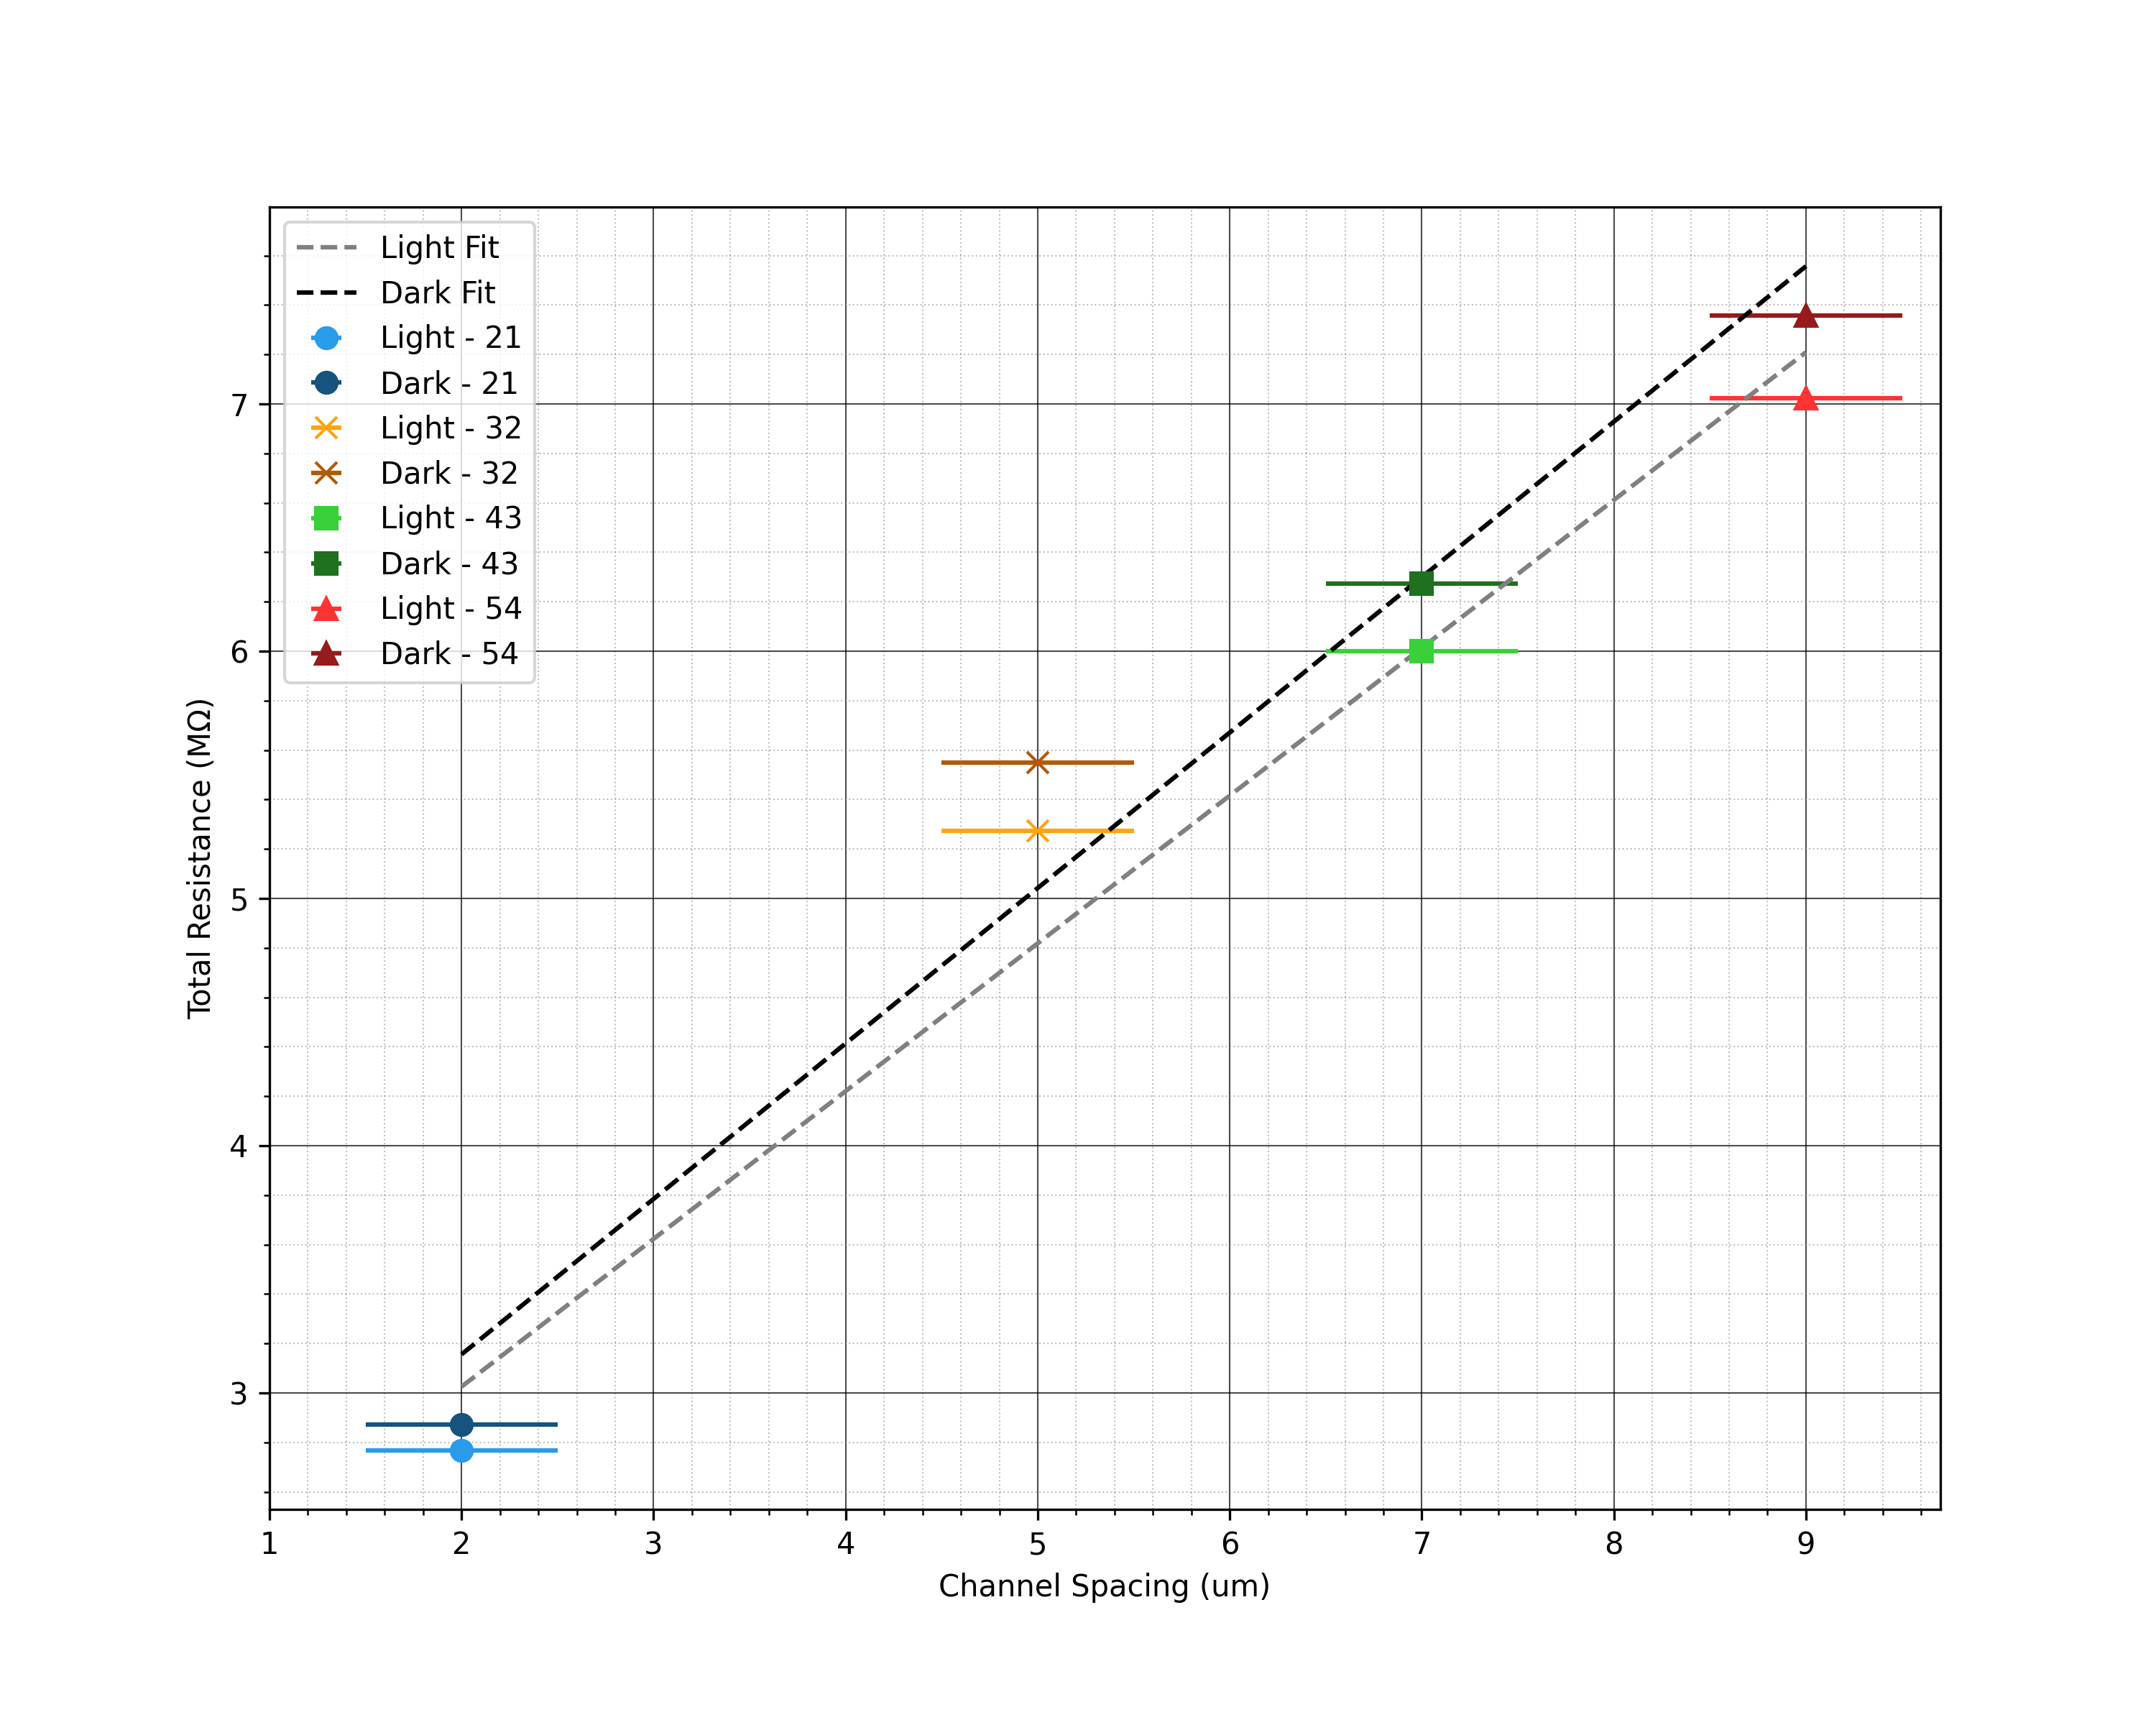
\includegraphics[width=\linewidth]{Chapter7/Figs/Raster/Lost Data/LTLM_graphite_mid(20V).png}
    \caption{A LTLM plot of the total measured resistance against LTLM channel spacing at 20~\si{\volt}, with lines of best fit for both the illuminated and dark datasets. Uncertainties due to the error associated with current measurements are not possible to see at this scale, $\pm0.5$~\si{\micro\metre} horizontal error bars are plotted.}
    \label{fig:lost_ltlm_20v}
\end{figure}

\begin{table}[h!]
\centering
\begin{tabular}{|c|c|c|}
\hline
\textbf{Parameter} & \textbf{Light} & \textbf{Dark} \\
\hline
R$^{2}$ & 0.969 & 0.966 \\
\hline
$R_{c}$ (\si{\kilo\ohm}) & $915$ & $949$ \\
\hline
$R_{s}$ (\si{\mega\ohm\per\sq]}) & $35.9$ & $37.7$ \\
\hline
$\rho_{c}$ (\si{\ohm\centi\meter\squared}) & 0.659 & 0.683 \\
\hline
$L_{t}$ (\si{\micro\meter}) & 1.53 & 1.51 \\
\hline
$\rho_{s}$ (\si{\ohm\centi\meter}) & 4300 & 4530 \\
\hline
\end{tabular}
\caption{LTLM Parameters at 20~\si{\volt} for light and dark conditions.}
\label{tab:lost_ltlm_parameters_20v}
\end{table}

Figure \ref{fig:lost_ltlm_20v} shows the results of plotting the total measured resistance at 20~\si{\volt} against the designed channel spacing (2, 5, 7 and 9~\si{\micro\metre}), with the data taken both under a bright light source and also in complete darkness represented. Error bars of $\pm0.5$~\si{\micro\metre} are plotted to account for the possible deviation of channel spacing as observed via optical characterisation. The extracted parameters are summarised in table \ref{tab:lost_ltlm_parameters_20v}.

\begin{figure}[H]
    \centering
    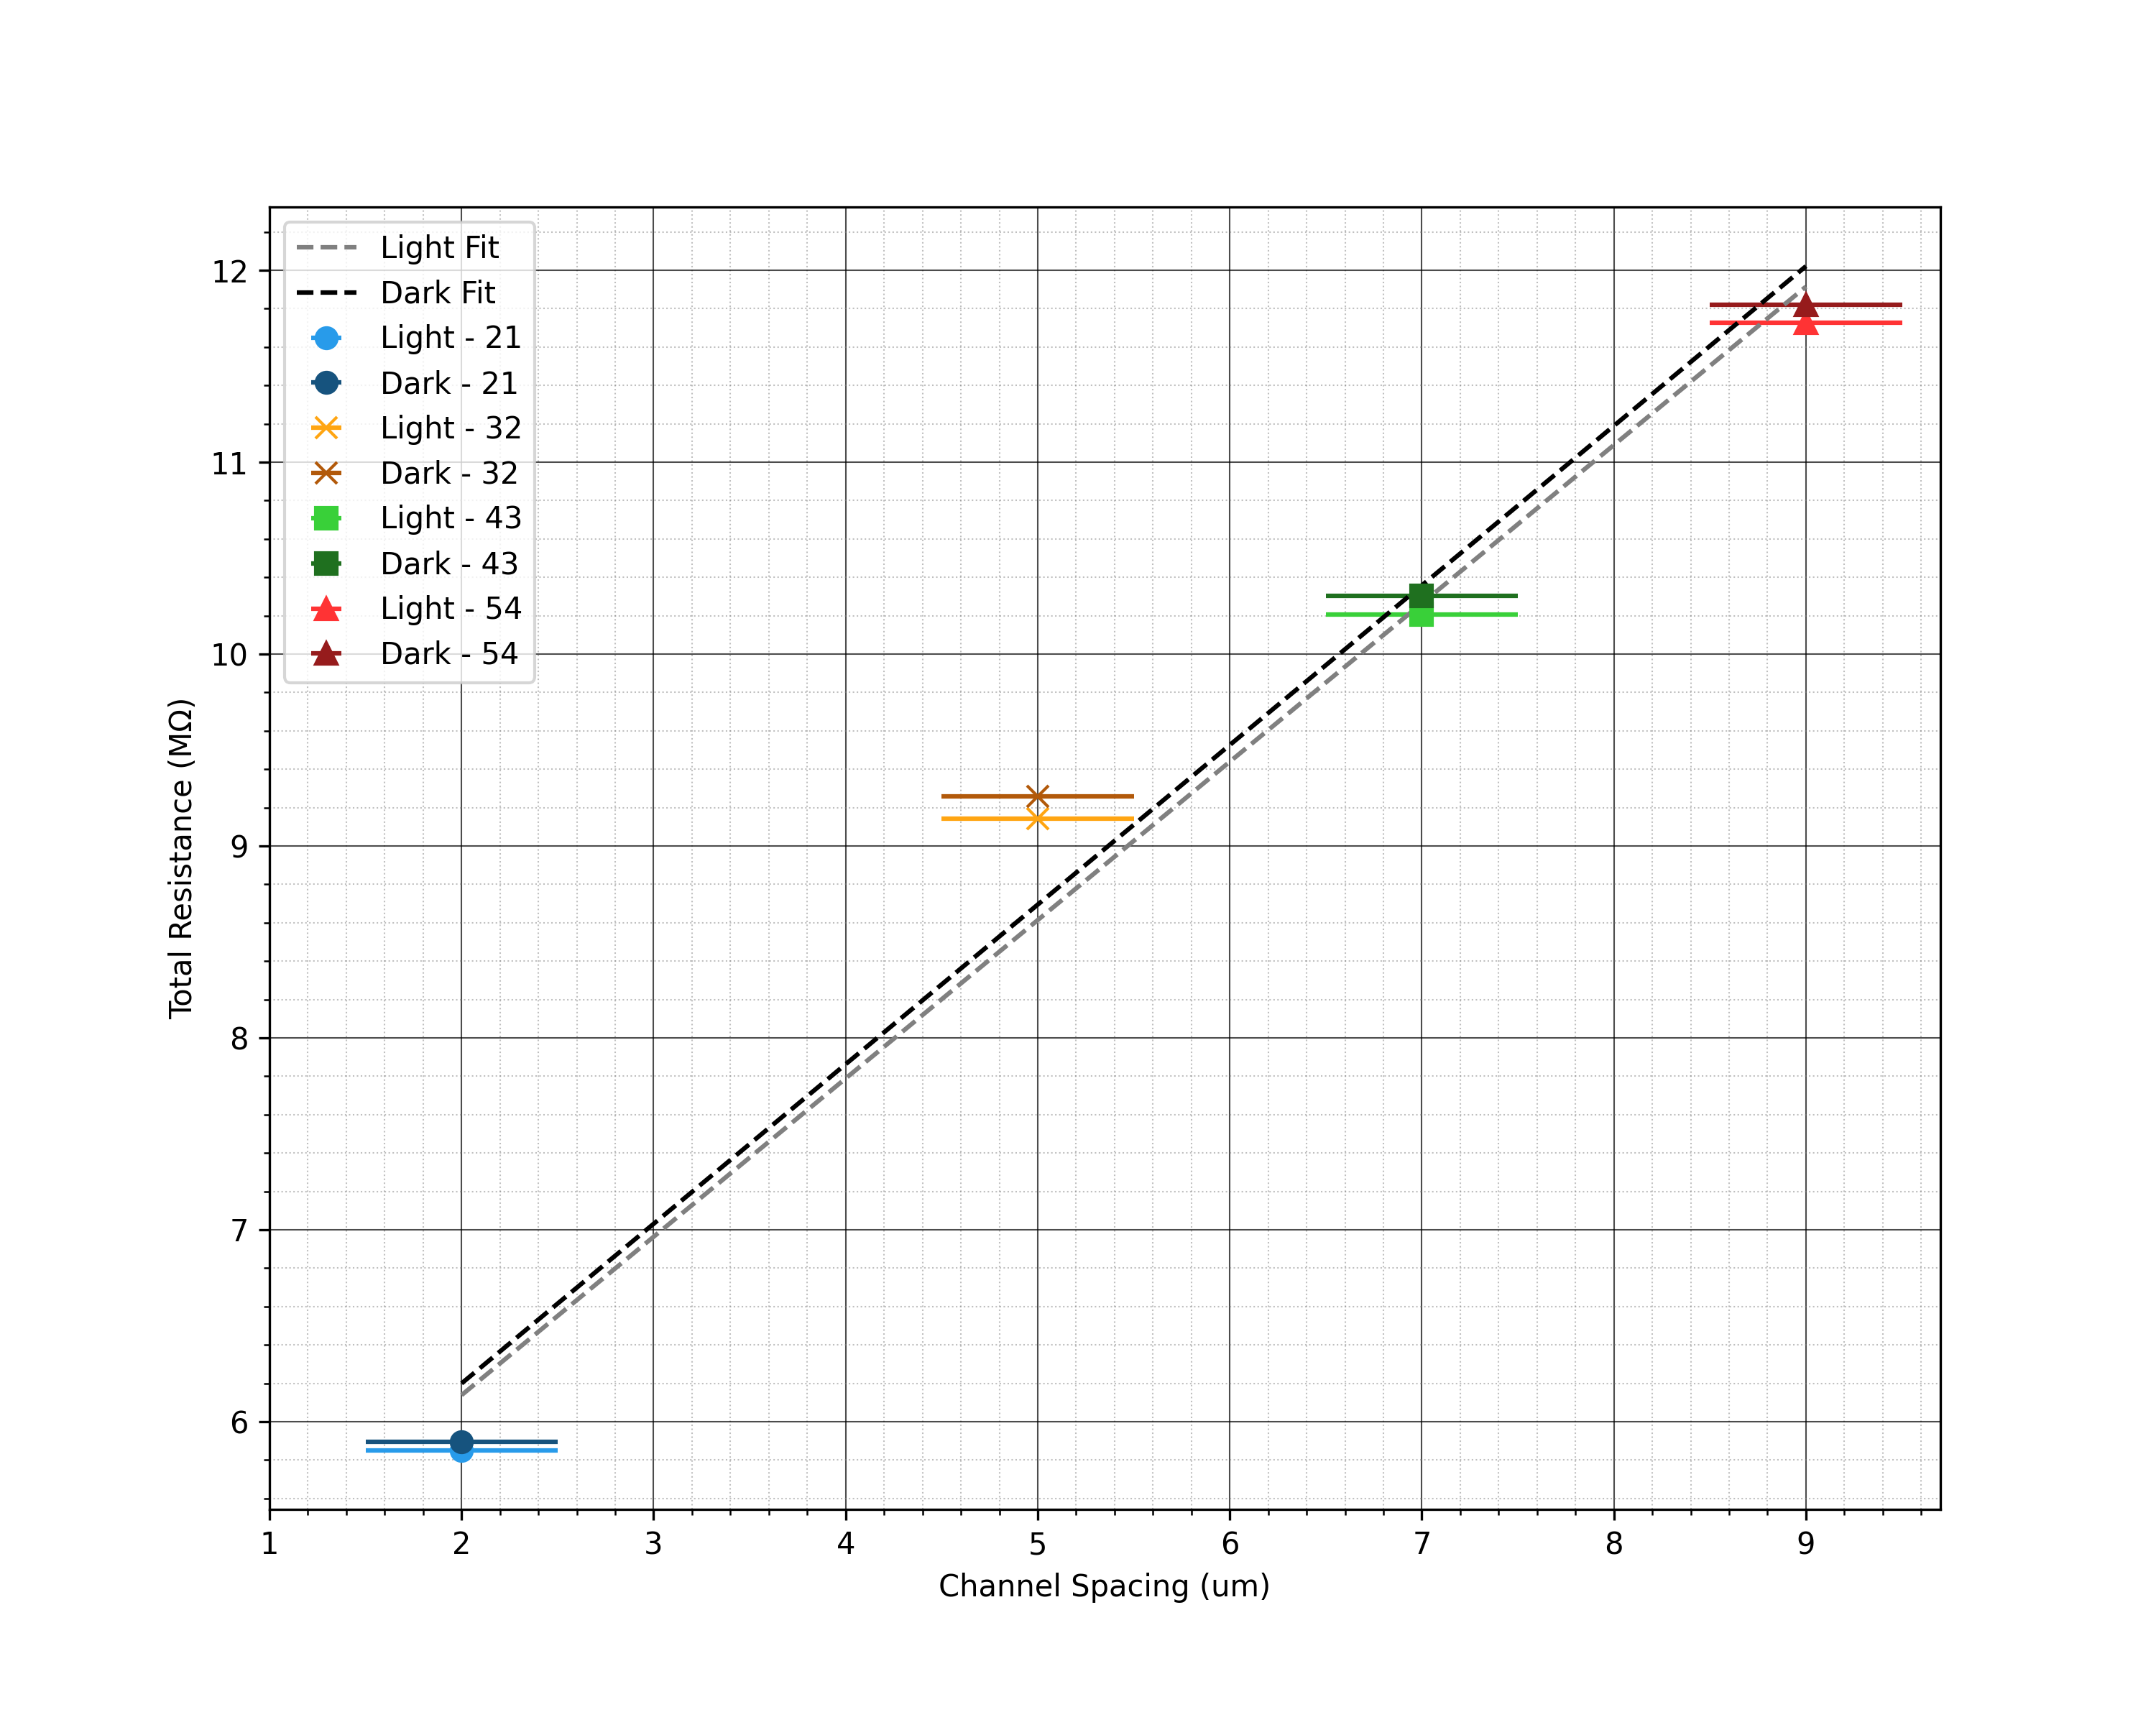
\includegraphics[width=\linewidth]{Chapter7/Figs/Raster/Lost Data/LTLM_graphite_mid(5V).png}
    \caption{A LTLM plot of the total measured resistance against LTLM channel spacing at 5~\si{\volt}, with lines of best fit for both the illuminated and dark datasets. Uncertainties due to the error associated with current measurements are not possible to see at this scale, $\pm0.5$~\si{\micro\metre} horizontal error bars are plotted.}
    \label{fig:lost_ltlm_5v}
\end{figure}

\begin{table}[h!]
\centering
\begin{tabular}{|c|c|c|}
\hline
\textbf{Parameter} & \textbf{Light} & \textbf{Dark} \\
\hline
R$^{2}$ & 0.978 & 0.976 \\
\hline
$R_{c}$ (\si{\kilo\ohm}) & $2244$ & $2268$ \\
\hline
$R_{s}$ (\si{\mega\ohm\per\sq}) & $49.5$ & $49.9$ \\
\hline
$\rho_{c}$ (\si{\ohm\centi\meter\squared}) & 1.62 & 1.63 \\
\hline
$L_{t}$ (\si{\micro\meter}) & 2.72 & 2.73 \\
\hline
$\rho_{s}$ (\si{\ohm\centi\meter}) & 5940 & 5990 \\
\hline
\end{tabular}
\caption{LTLM Parameters at 5~\si{\volt} for light and dark conditions.}
\label{tab:lost_ltlm_parameters_5v}
\end{table}

Figure \ref{fig:lost_ltlm_5v} shows a LTLM plot for total resistance as measured at an applied bias of 5~\si{\volt} against the designed channel spacing (2, 5, 7 and 9~\si{\micro\metre}), with the data taken under both a bright light source and also in complete darkness represented. Error bars of  $\pm0.5$~\si{\micro\metre} are plotted to account for the possible deviation of channel spacing as observed via optical characterisation. The extracted parameters are given in table \ref{tab:lost_ltlm_parameters_5v}. The change in specific contact resistivity is quite natural, as it may be interpreted as mostly being due to the image force barrier lowering of the forwardly biased Schottky barrier in the double Schottky structure \cite{sze2006, Aubry1994}. There is the additional factor of greater donor ionisation under increasing electric field strengths that may also be considered as a factor, since the majority of substitutional phosphorous dopants are effectively frozen out at room temperature \cite{koizumi1997, Donato2018, donato2019}. The concentration of dopants is a key factor in the formation of conventional ohmic contacts on semiconductors, and this may hence be visible here.

\subsection{Voltage Dependent specific contact resistivity}

\begin{figure}[H]
    \centering
    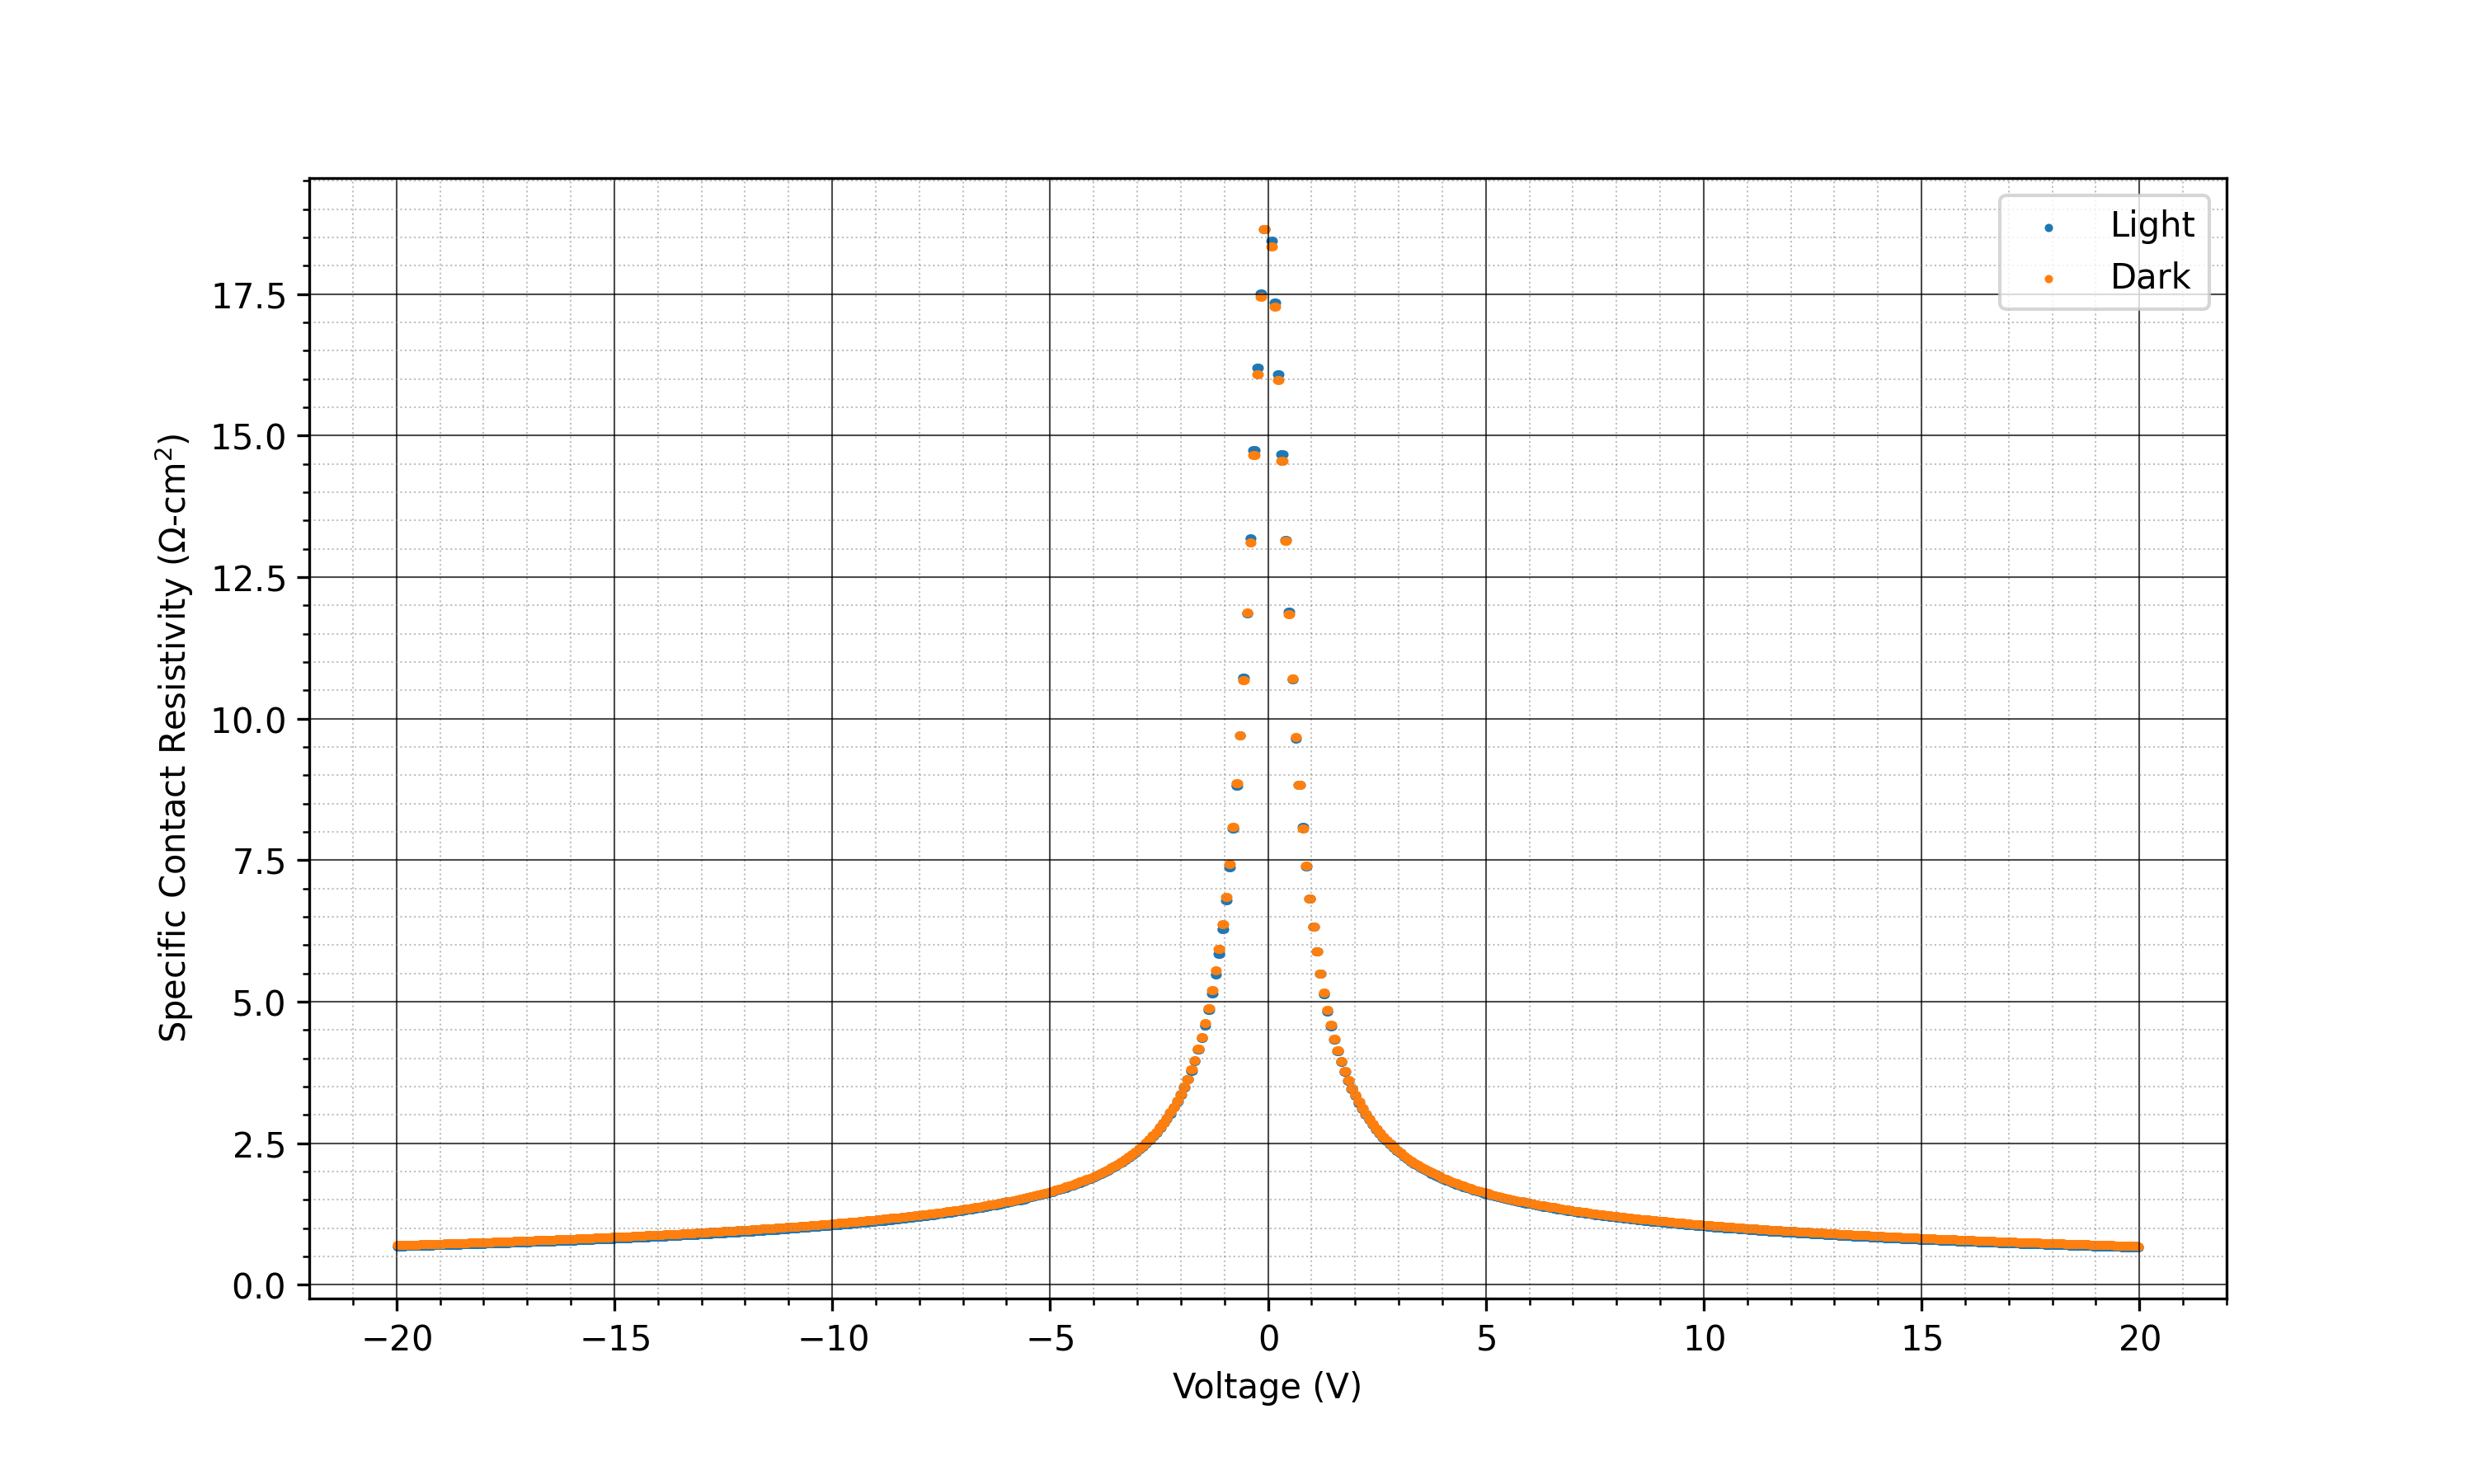
\includegraphics[width=\linewidth]{Chapter7/Figs/Raster/Lost Data/LTLM_rhoc_plot.png}
    \caption{A plot of the measured specific contact resistivity as a function of applied voltage, sampling the full range of IV characteristics.}
    \label{fig:lost_ltlm_rhoc}
\end{figure}

Finally, figure \ref{fig:lost_ltlm_rhoc} provides a visual representation for the dependence of specific contact resistivity upon the applied voltage across the device. Notably, even in the very low voltage region approaching 0~\si{\volt}, the specific contact resistivity remains below 20~\si{\ohm\centi\metre\squared}. This is quite unexpected, as the IV characteristics would initially indicate that the low voltage region has a very high resistance. Instead, it is clear that the double Schottky structure here allows for a measurable level of leakage current even without either contact being in the forward bias mode of operation. The difference between measurements taken under direct illumination and in complete darkness are difficult to pick apart in figure \ref{fig:lost_ltlm_rhoc}, but there is a mean difference between the light and dark data of $-0.0228$~\si{\ohm\centi\metre\squared}, with a variance of $0.0003$~\si{\ohm\squared\centi\metre\tothe{4}}. The negative mean difference indicates that the dark specific contact resistivity is higher than that of the well lit measurements, and the variance is low enough to consider the majority of data in this voltage range to agree with this mean difference. For a final check, a comparison between all pairs of data-points was conducted to find any dark values which were less than that of the light measurements. All such values are contained within the $\pm1.08$~\si{\volt} range, as could be expected based on the divergence of IV characteristics beyond 1~\si{\volt}.

Throughout all of the data presented for the second round of LTLM measurements, the error can be estimated via the previously discussed estimates of error via exact probe positioning on the laser processed wires. The systematic error present for these measurements is estimated to be approaching the limit imposed by the B1500 probe station, which is well below even 1\% of the currents measured here.

\begin{comment}
  Before examining the emitter structures designed to take advantage of geometrically enhanced field effect emitters, at this point it is necessary to consider theoretical models of the double Schottky device structure, which may also be described as a back-to-back Schottky junction. This will provide the necessary framework for understanding the difference between thermionic and field effect emission characteristics.  
\end{comment}

\printbibliography[heading=subbibliography]

\end{refsection}